\documentclass[a4paper,12pt]{book}
\usepackage{bm}
\usepackage{siunitx}
\usepackage{cases}
\usepackage[english]{babel}
\usepackage[dvipdfmx]{graphicx}
\usepackage{subfig} 
\columnsep 3zw
\renewcommand\baselinestretch{0.8} 
\topmargin -1.5cm        % read Lamport p.163
\oddsidemargin -0.04cm  % read Lamport p.163
\evensidemargin -0.04cm  % same as oddsidemargin but for left-hand pages
\textwidth 16.59cm
\textheight 23.50cm 
% \pagestyle{empty}       % Uncomment if don't want page numbers
\parskip 7.2pt           % sets spacing between paragraphs
% \renewcommand{\baselinestretch}{1.5} 	% Uncomment for 1.5 spacing between lines
\hyphenpenalty=2000\relax
\exhyphenpenalty=2000\relax
\sloppy
\title{\Large Graduate School of Sciences and Technology for Innovation, Yamaguchi University\\[1cm]
Division of Fundamental Sciences\\[3cm]
\huge A Computational Model of Cell Migration of Fish Keratocytes\\[5cm]
}
\author{Yu Tokunaga}
\date{\Large \today}
\begin{document}
\pagenumbering{roman}
\maketitle
\setcounter{page}{1}
\tableofcontents
\chapter{Introduction}
\pagenumbering{arabic}
\setcounter{page}{1}
\section{Introduction}
%問題提起
{\it Amoeba proteus}, a common ameba cell, migrates by stretching pseudopodia and its cell shape continuously changes.
In contrast, keratocyte, a fish epidermal cell, migrates while keeping its half-moon shape.
Keratocytes in the initial state is a circular shape and deforms in a half-moon shape when moving.
It is not clear why keratocytes form a half-moon shape and migrate without changing its shape.

%いかに不思議か(問題点を具体化)
Migrating cells including keratocytes perform cell migration by the action of cytoskeleton called actin molecule. 
Actin polymerization (AP) is a phenomenon in which actin molecules overlap each other to form F-actin. 
F-actin is shortened in length by depolymerization or lengthened by AP.
F-actin that repeats elasticity pushes the cell membrane and deforms the cell.
If the AP is too active, the cell membrane will swell up.
Conversely, without an AP, the cell membrane will not be deformed.
It can be seen that it is difficult to keep the shape of cells during cell migration even by paying attention to one element called AP.

%目的
The porpose of this study is to clarify the relationship between keratocytes morphology and motor function in cell migration. Specifically, we will elucidate the intracellular mechanism that keeps the cell shape half-moon during cell migration.

%本稿の構成
The structure of this paper is as follows. In Chapter 2, we explain the specific features of keratocytes and the outline of cell migration mechanism. In Chapter 3, details of simulation experiment method will be described. Section 4 presents the results of simulation experiments and discusses the considerations. In the last chapter, we explain the improvements and future prospects of the facts and methods obtained from this survey.

%第2章
\chapter{Keratocytes}
\section{Characteristics of Cell Migration of Keratocytes}
\begin{figure}[tbp]
\centering
\includegraphics[scale=0.4]{kera.eps}
\caption{Keratocytes during cell migration.(Source: Takako Tanaka, Iwadate Lab).}
\label{fig:kera}
\end{figure}

%ケラトサイトの自己紹介
Keratocytes is migratory fish epidermal cells, is about \SI{70}{\mu m} in size and present on the back side of the fish scales.
When a fish bleeds due to trauma, they gather to cover the wound.
Although the locomotion of keratocytes is one of amoeboid movements, however, it is different from typical amoeba movement and moves straight with keeping a half-moon shape.
Migrating cells are cells that can freely move around in the same way as lymphocytes.
Keratocytes advances by about one body length in one minute.
The physiological findings of cell migration will be introduced in the next section.

%参考文献
Svitkina et al. \cite{svitkina1997analysis} showed that the forward translocation of the cell body and retrograde flow in the lamellipodia are both driven by contraction of an actin-myosin network in the lamellipodial/cell body transition zone.
The importance of both actin polymerization (AP) and actin retrograde flow (ARF) in cell migration of migrating cells was suggested.
Asano et al. \cite{asano2004keratocyte} showed that movement similar to keratocytes was observed when AmiB gene was deleted from ameba cells of cellular slime mold {\it Dictyostelium discoideum} which performs typical ameba movement.
Even in other ameboid cells, if some condition is satisfied, there is a possibility of maintaining a half-moon shape, which means that morphogenesis of keratocyte is not unique to keratocyte and is a physical mechanism causing cell migration.
Therefore, this research strongly insists that the crescent shape morphogenesis is a physical factor such as AP and ARF.
Nakata et al. \cite{nakata2016role} focused on pulling force against temperament and flow rate gradient of ARF, and reported that stress fiber (SF) plays an important role in morphological control of keratinocytes.
Focusing on the fact that the keratocytes of different fish are not in the same crescent shape, it was suggested that the factor is the velocity gradient of ARF.
Swaminathan et al. \cite{swaminathan2017actin} focused on adhesion receptor integrins that bind cells and their environment.
Suggesting that regurgitation of actin regulates the orientation of the integrin and may determine the propulsion direction of the cell. From the previous studies above, it is known that both AP and ARF play an important role in cell migration of keratocytes.
Okimura et al. \cite{okimura2018rotation} showed that the rotation of these stress fibers plays the role of a “wheel” in crawling migration of keratocytes.
Removal of the stress fibers decreased migration velocity and induced the collapse of the left-right balance of crawling migration.
It is suggested that cell migration is not performed only by AP and ARF but SF located in the posterior part of the cell is also important.

\section{Molecular Mechanism of Cell Migration}
A cell has a structure called a cytoskeleton. The cytoskeleton is like bones for humans, but in contrast to static human bones, the cytoskeleton is dynamic and is an important organelle that maintains the shape of the cell. The main component of the cytoskeleton is the actin molecule. As the actin molecule polymerizes and depolymerizes, the shape of the cell membrane changes. The actin molecule is elongated by polymerization in the cell membrane but retreats in the direction opposite to the elongation direction by the bundle of actomyosin called stress fiber. This phenomenon is called actin retrograde flow, and it is not clear what kind of role it plays in cell migration. The cell membrane extruded by polymerization of the actin molecule becomes the pseudopodia and adheres to the substrate at the advancing position. Thereafter, the adhesion between the substrates of the rear cell membrane is released and dragged forward. By repeating this cycle, cell migration mechanism is formed.

It is a common fact even in keratocytes that the cell membrane is deformed by actin molecule polymerization. In the simulation experiment described in the next chapter, we investigate how the cell membrane forms a half moon shape when actin molecule polymerization acts on the cell membrane.


\chapter{Simulation Methods}
\section{Simulation Methods of Cell Membrane Molecules}
In the cell membrane model, each cell membrane molecule moves under the resultant of force and velocity from the actin molecule and resistance force proportional to force between the cell membrane molecules. The equation of motion of the cell membrane molecule is as follows.
\begin{equation}
m\frac{d^2\bm{x}_i}{dt^2} = \bm{F}^m_i +  \bm{F}^a_i - \eta \frac{d\bm{x}_i}{dt}
\end{equation}
where  $m$ is the mass, $\eta = 8.9\times10^{-6}\si{~kg/s}$ is the viscous coefficient, and $\bm{x}_i$ is the position vector of the membrane molecule. The membrane molecule has the force  $\bm{F}^m_i$ received from the membrane molecule and the force  $\bm{F}^a_i$ received from the actin molecule. It is assumed that the force  $\bm{F}^m_i$ acting between the membrane molecules can be represented by elastic force:
\begin{equation}
\bm{F}^m_i = \sum_{i \in I_j}  -k((\bm{x}_j -\bm{x}_i )-\bm{l}_{ij} )
\end{equation}
where $k$ is the spring constant, and $\bm{l}_{ij}$ is the natural length between the membrane molecules $i-j$. Molecule  $i$ belongs to the set of index $I$ adjacent to molecule $j$. However, this natural length measures the distance between the membrane molecules in the initial state. The force  $\bm{F}^a_i$ that a membrane molecule receives from an actin molecule is assumed to be the repulsive force:
\begin{equation}
\bm{F}^a_i = \sum_{\{ \forall i | \| \bm{x}_j - \bm{B}_i \|<D_2\}} \frac{s}{\|\bm{x}_j -\bm{B}_i \|} \frac{\bm{x}_j -\bm{B}_i }{\|\bm{x}_j -\bm{B}_i \|}
\end{equation}
where $s$ is a constant that determines the strength of the repulsive force, and $D_2$ is a distance range to receive a force.


\section{Simulation Methods of Actin Molecules}
\subsection{Actin Polymerazation}
The polymerization of actin has polarity, the end where polymerization is carried out is called barbed-end, and the end which is not done is called pointed-end. Since polymerization is carried out well in a region where many actin molecules are present , the polymerization rate is proportional to the actin concentration in the vicinity.  The filament formed by actin polymerization is called F-actin. F-actin on the simulation is treated as a rod. F-actin is defined as the position vector at both ends of the rod.
Here, the position vector of pointed-end of particle $i$ is $\bm{P}_i$, and the position vector of barbed-end of particle $i$ is $\bm{B}_i$.
$\bm{P}_i$ and $\bm{B}_i$ are updated step by step to control polymerization and depolymerization.

As described above, the polymerization direction $\bm{L}_i$ is determined at the initial stage of cell migration.Therefore, the formula for updating the polymerization is \[\bm{B}_i \gets \bm{P}_i + \bm{L}_i\]. However, considering the surrounding actin concentration and time step, the formula can be rewritten as follows.
\begin{equation}
\bm{B}_i \gets \bm{P}_i + f^p(c)\bm{L}_i \cdot dt
\end{equation}
where $f^p(c) = 5.0 \cdot \exp{\frac{c}{10.0}}$ is a function that  increases exponentially with actin concentration $c$ and $dt$ is the time step.

Regarding depolymerization, the update formula is as follows.
\begin{equation}
\bm{P}_i \gets \bm{P}_i + f^d(c)\bm{L}_i \cdot dt
\end{equation}
where  $f^d(c) = \frac{5.0}{c}$ is a function inversely proportional to $c$. However, these formulas are not done every time, but are done with probability \[p_i(c) = c_i = \frac{a_i}{N}\] where $p_i(c)$ is the probability that depends on the concentration $c_i$ in region $i$, $a_i$ is the number of actin in region i, and $N$ is the total number of actin. In this simulation, the original space was divided into 3600 spaces($i=3600$).


\subsection{Actin Retrograde Flow}
Because ARF is often unknown, we simulate with some assumptions. Although the element that causes ARF is a stress fiber, since the cell model of this paper does not introduce a stress fiber, it substitutes the membrane molecule at the end of the cell membrane. Since it is not clear how much the effect on actin molecule also works, it was assumed that the closer to the membrane molecule the stronger the effect.

The cell membrane molecule with the smallest x coordinate is the reference point $\bm{E}_0$. The calculation formula for implementing ARF is shown below.

\begin{numcases}
  {}
  \bm{B}_i \gets \bm{B}_i - \alpha \frac{ \bm{B}_i - \bm{E}_0}{{\| \bm{B}_i - \bm{E}_0 \|}^w} & \\
   \bm{P}_i \gets \bm{P}_i - \beta \frac{ \bm{P}_i - \bm{E}_0}{{\| \bm{P}_i - \bm{E}_0 \|}^w} &
\end{numcases}
where the vector $\bm{B}_i$ is barbed-end, the vector $\bm{P}_i$ is pointed-end, and $\alpha$ and $\beta$ are constants that determines the strength of the ARF. This equation means ARF which does not depend on distance when w = 1 and ARF depending on distance when w = 2.

Since there is a possibility that the shape of the cell membrane may change at the position of the reference point $\bm{E}_0$, another reference points $\bm{E}_1$ and $\bm{E}_2$ are proposed. Hence, two pattern experiments are performed with one and two ARF reference points. As shown in the figure, the reference points A and B are positioned at 1/5 of the cell membrane. The position update formula of ARF when two reference points  $\bm{E}_1$ and $\bm{E}_2$ are used is shown below.

\begin{numcases}
  {}
  \bm{B}_i \gets \bm{B}_i - \gamma \left( \frac{ \bm{B}_i - \bm{E}_1 }{{\| \bm{B}_i - \bm{E}_1 \|}^w} + \frac{ \bm{B}_i - \bm{E}_2}{{\| \bm{B}_i - \bm{E}_2 \|}^w} \right)& \\
   \bm{P}_i \gets \bm{P}_i - \delta \left( \frac{ \bm{P}_i - \bm{E}_1 }{{\| \bm{P}_i - \bm{E}_1 \|}^w} + \frac{ \bm{P}_i - \bm{E}_2}{{\| \bm{P}_i - \bm{E}_2 \|}^w}  \right) &
\end{numcases}
where $\gamma$ and $\delta$ are constants that determines the strength of the ARF.

In the above equation, the denominator is squared taking into consideration the distance dependency between the particles. If we compare distance-dependent ARF and distance-independent ARF, the square of the denominator of the above equation is deleted.
\section{Initial Condition and Relocation  Condition}
\begin{figure}[tbp]
\centering
\includegraphics[scale=0.25]{top.eps}
\caption{Top view of keratocyte model at time $t=0$.}
\label{fig:top0}
\end{figure}
\begin{figure}[tbp]
\centering
\includegraphics[scale=0.25]{side.eps}
\caption{Side view of keratocyte model at time $t=0$.}
\label{fig:side0}
\end{figure}
The total number of actin is 3000, the number of membrane molecules is 2000. When updating the position of F-actin every step, deformation of the cell membrane can not catch up. Therefore, the position of the cell membrane molecule is updated each time, and the position of actin molecule is updated once every 10 times.

The direction of polymerization is randomly determined. Some actins invade areas where they can not normally invade due to the progress of polymerization. For example, it is outside the cell membrane and in the nucleus. In such a case, relocation processing is applied to the actin. F-actin escaping from the cell membrane disappears and moves to a random place close to the cell membrane. The region to be repositioned is outside of the cell membrane and regions where the concentration of actin molecule is low.

The initial state in the simulation experiment is shown in Fig. \ref{fig:top0} and Fig. \ref{fig:side0}. The actin molecule is indicated by a green line, and the cell membrane is indicated by a white dot. This is the initial placement of actin molecules because the nucleus is present in the center of the cell and the actin molecule is distributed a lot in the anterior direction. The membrane molecules are placed on the surface of the cylinder and not inside.

\section{Reduction in Calculation Volume}
%細胞膜のはなし
Calculating the distance between membrane molecules in all steps increases the computational complexity.
Therefore, when calculating the cell membrane model, the distance between the cell membrane molecules stored in advance was referred to.
In the initial state, the index information of the adjacent cell membrane molecules was stored.
This method can be adopted because the position information adjacent does not change regardless of how much the interparticle distance changes.

%エリアわけ
Likewise, if the distance between the cell membrane molecule and the actin molecule is calculated in all steps, the process becomes heavy.
Unlike the case of intermolecular molecules, the index information of nearby molecules changes in the case of actin molecule and cell membrane molecules.
For this reason, the simulation space was divided into areas in mesh form, and index information of molecules in the same area was saved.


\chapter{Results and Discussion}
\section{Simulation Results}
\subsection{Role of Actin Retrograde Flow}

\begin{figure}[h]
 \subfloat[t=0.5.]{%
  \begin{tabular}{c}
   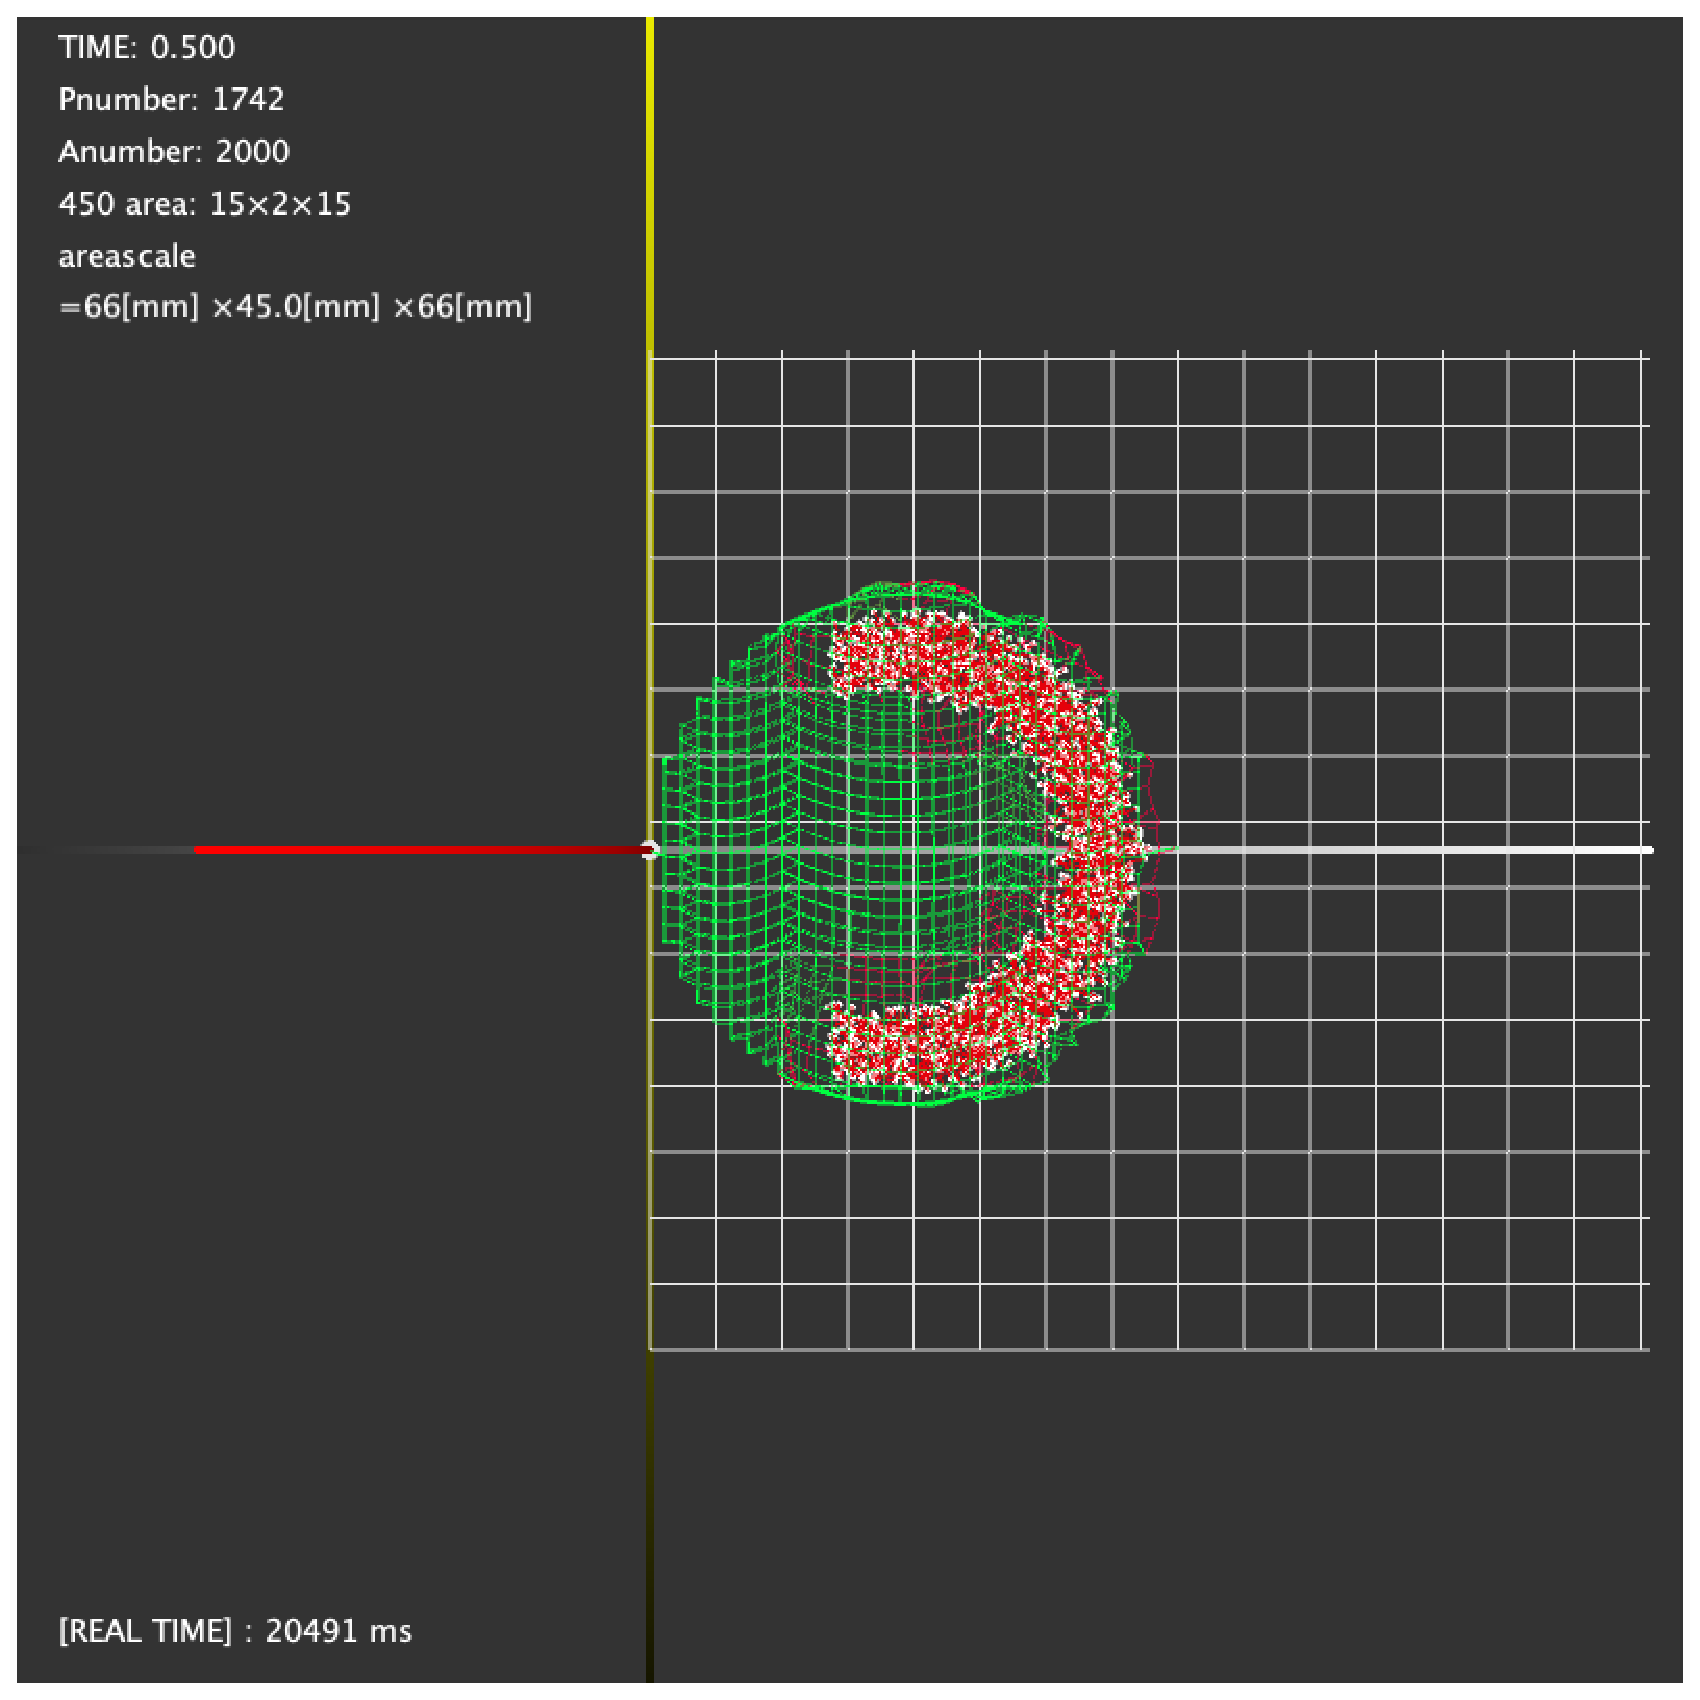
\includegraphics[width=5cm]{top05_arf.eps} \\
   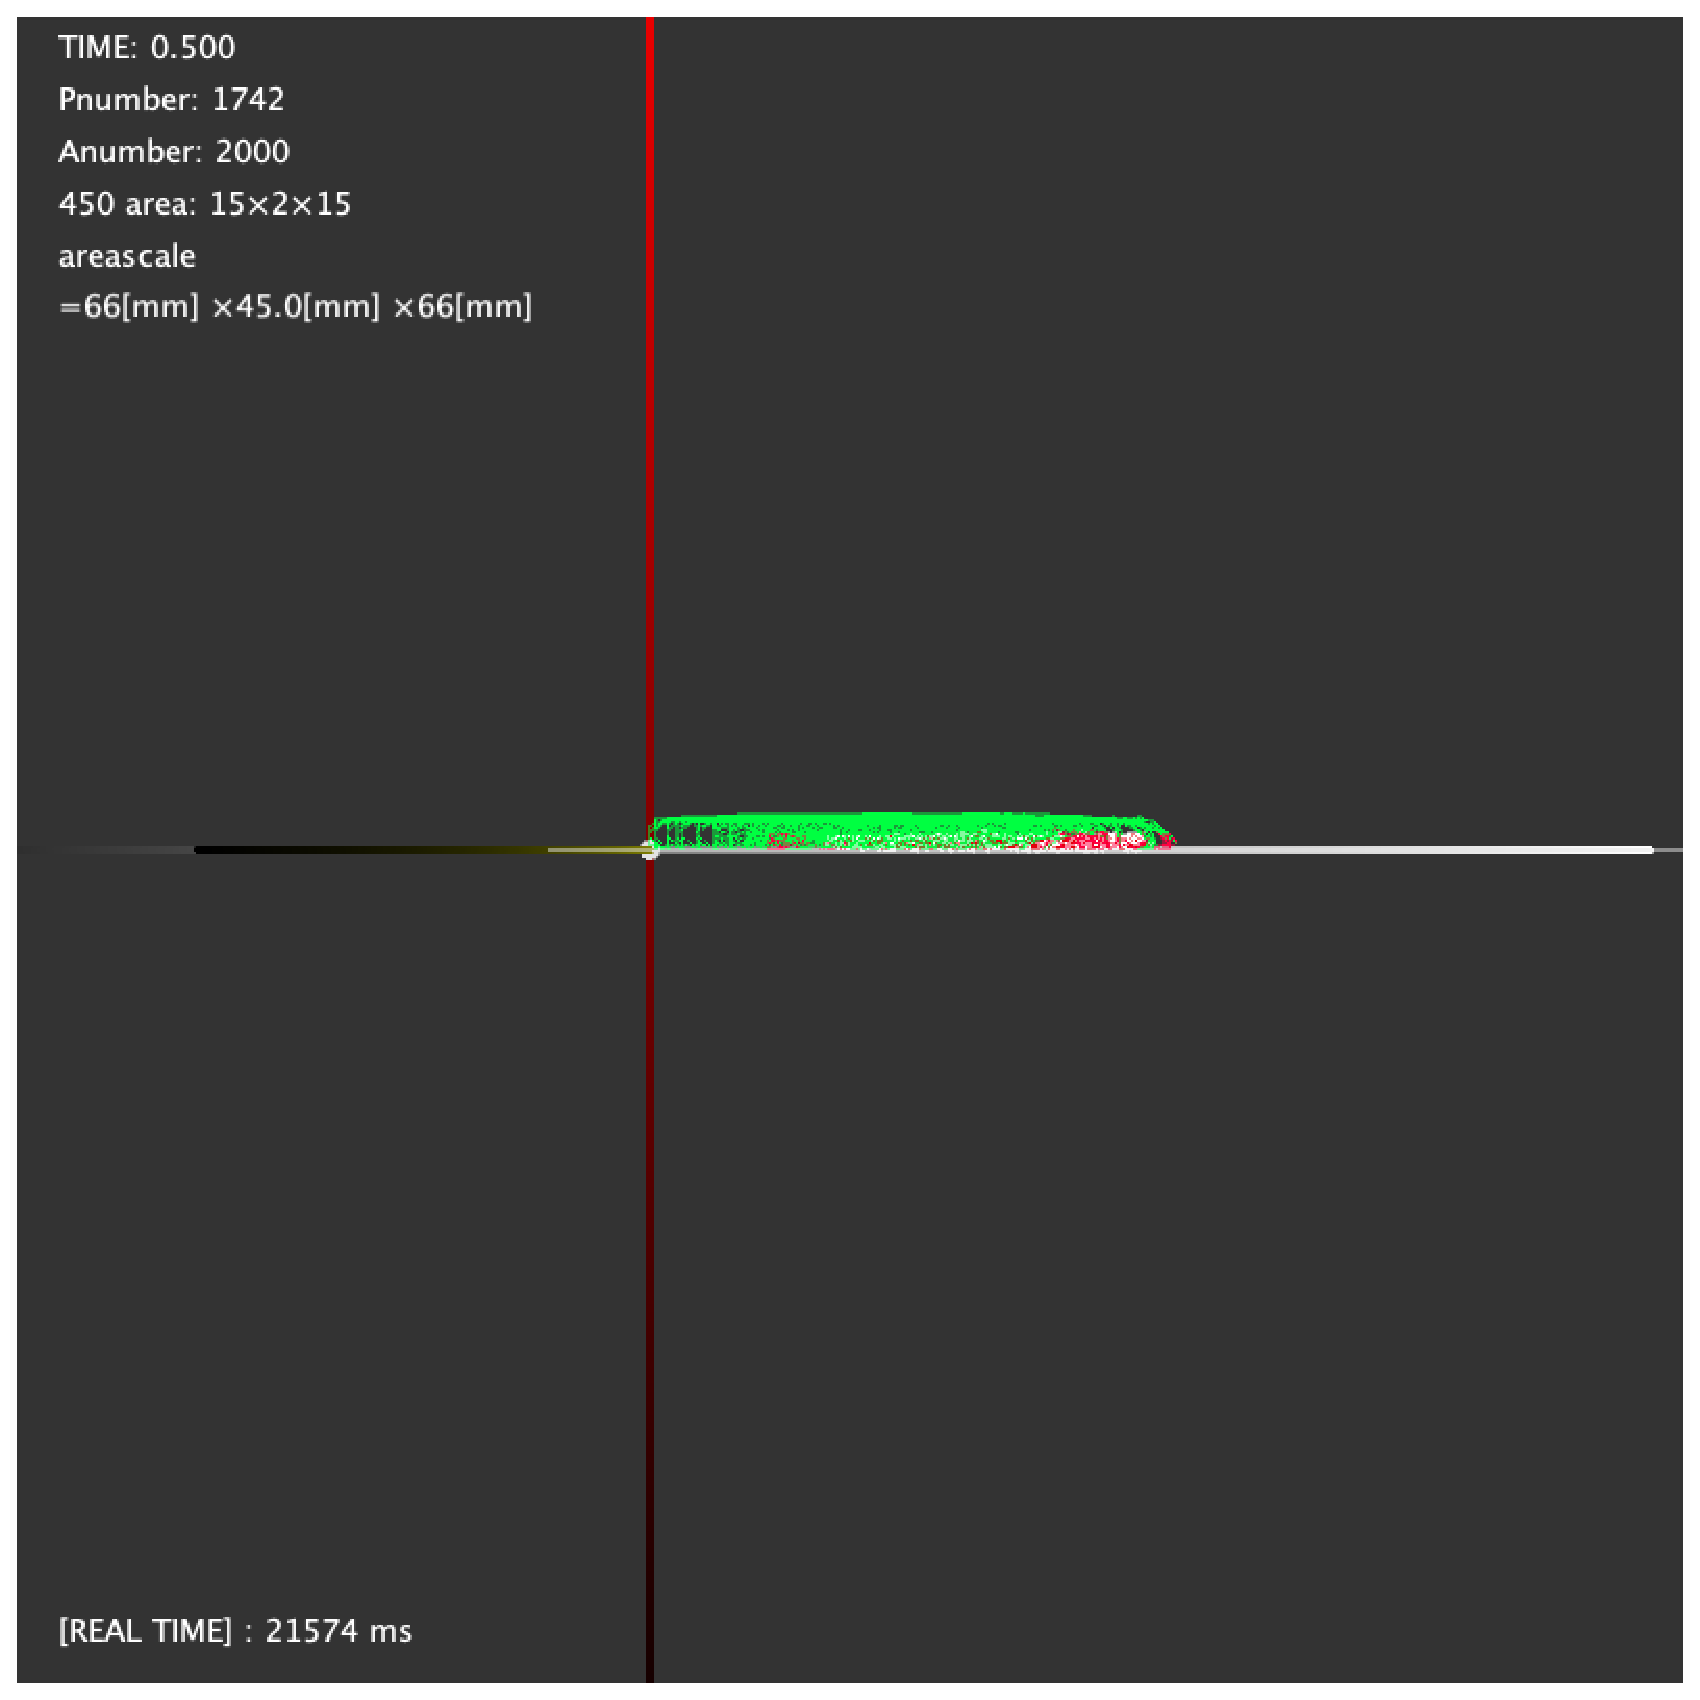
\includegraphics[width=5cm]{side05_arf.eps}
  \end{tabular}
 }%
 \subfloat[t=2.0]{%
  \begin{tabular}{c}
   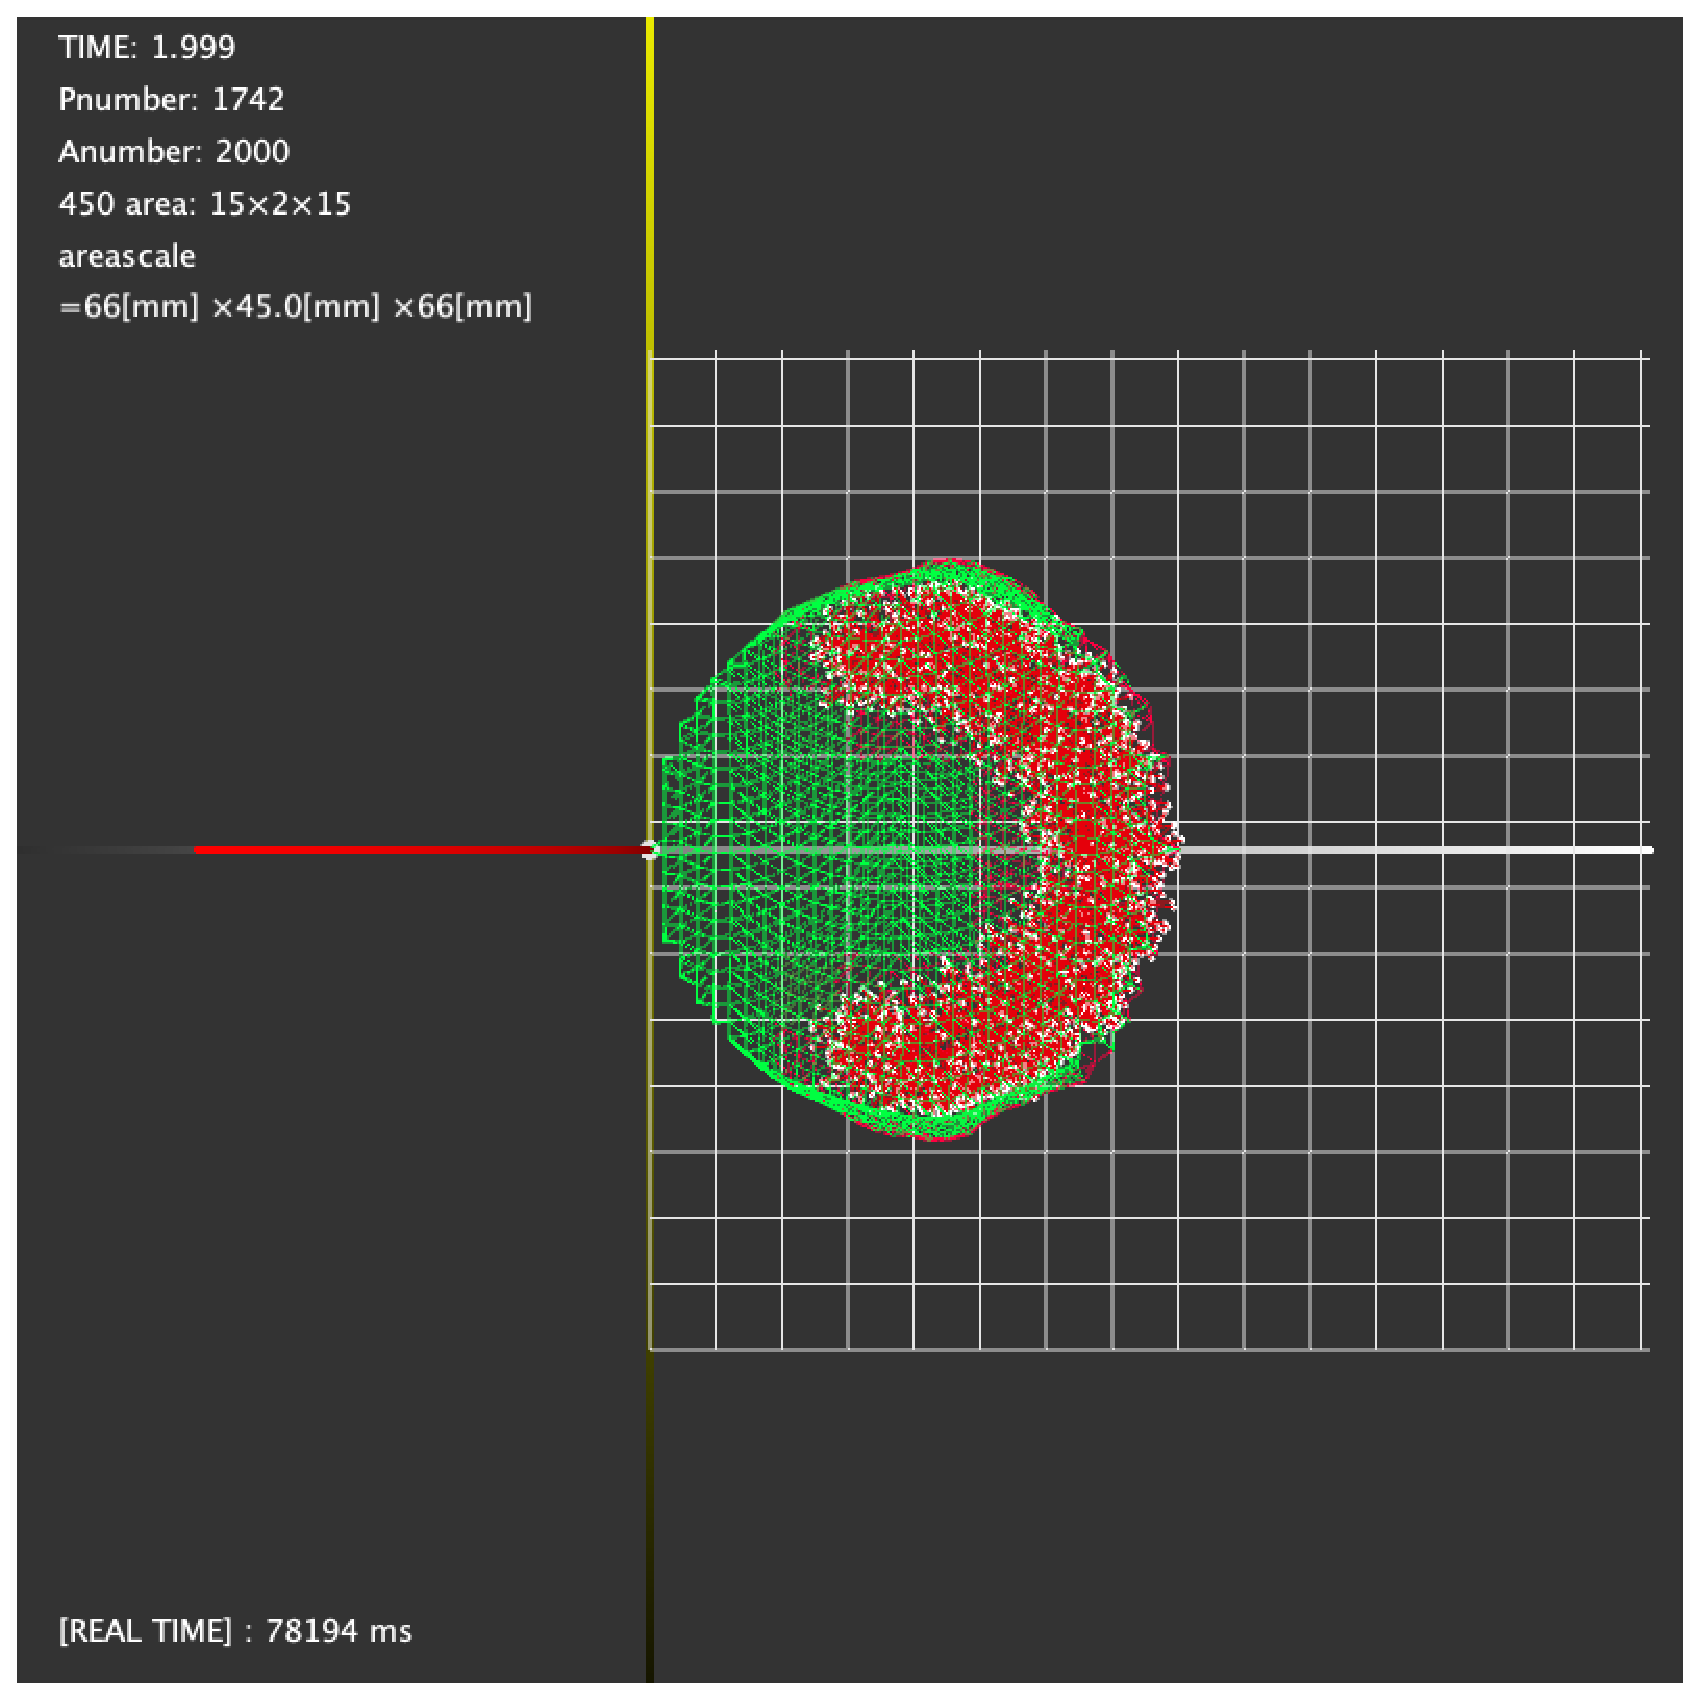
\includegraphics[width=5cm]{top20_arf.eps} \\
   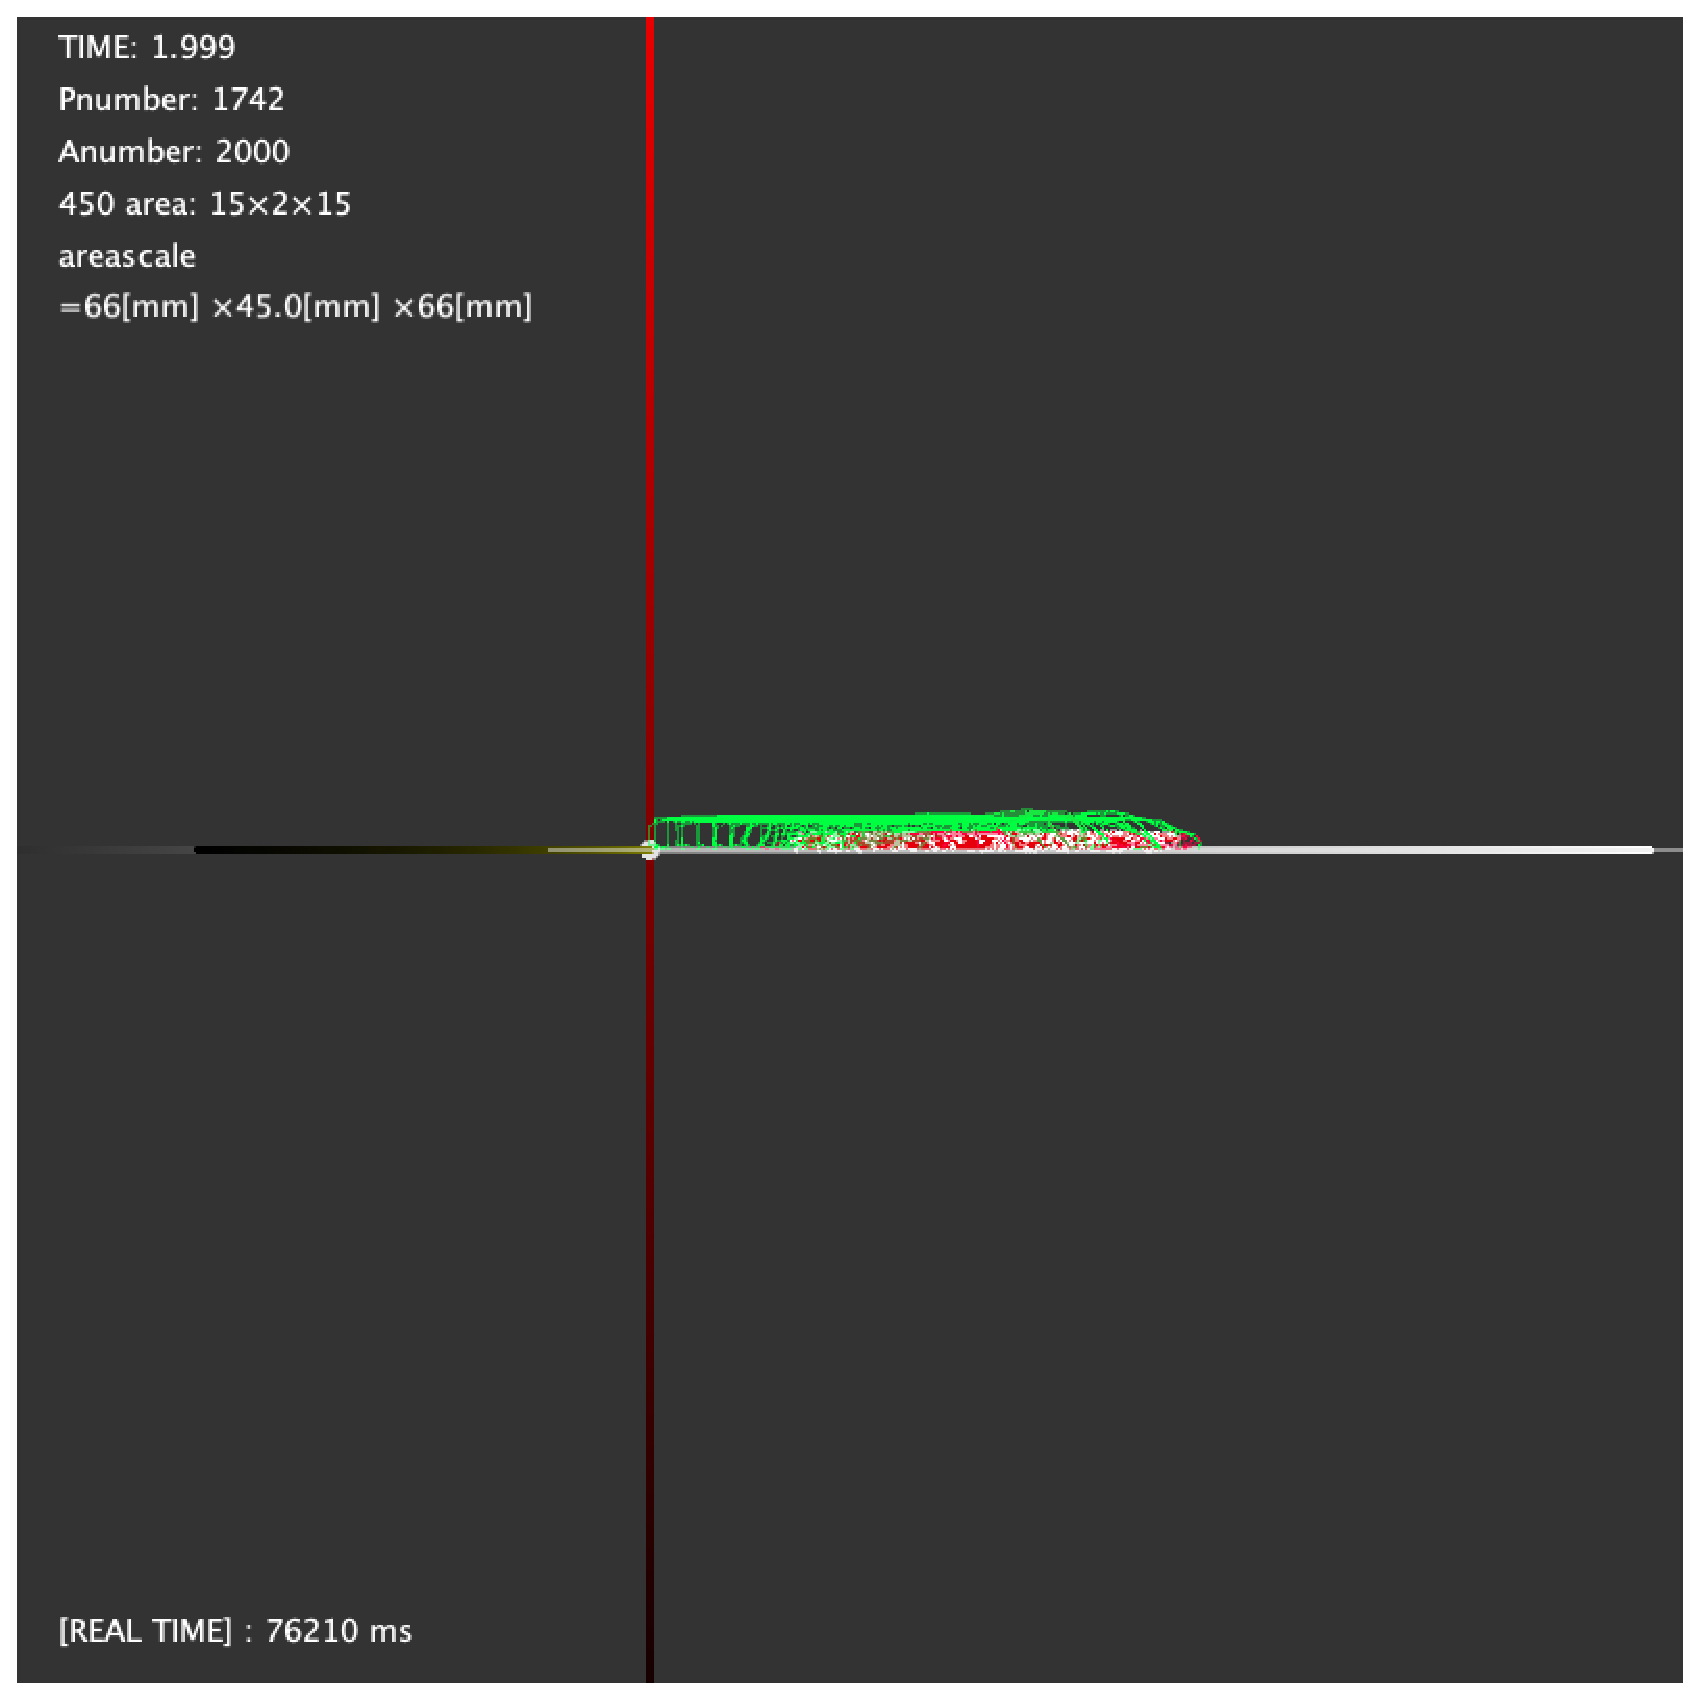
\includegraphics[width=5cm]{side20_arf.eps}
  \end{tabular}
 }%
 \subfloat[t=4.0]{%
  \begin{tabular}{c}
   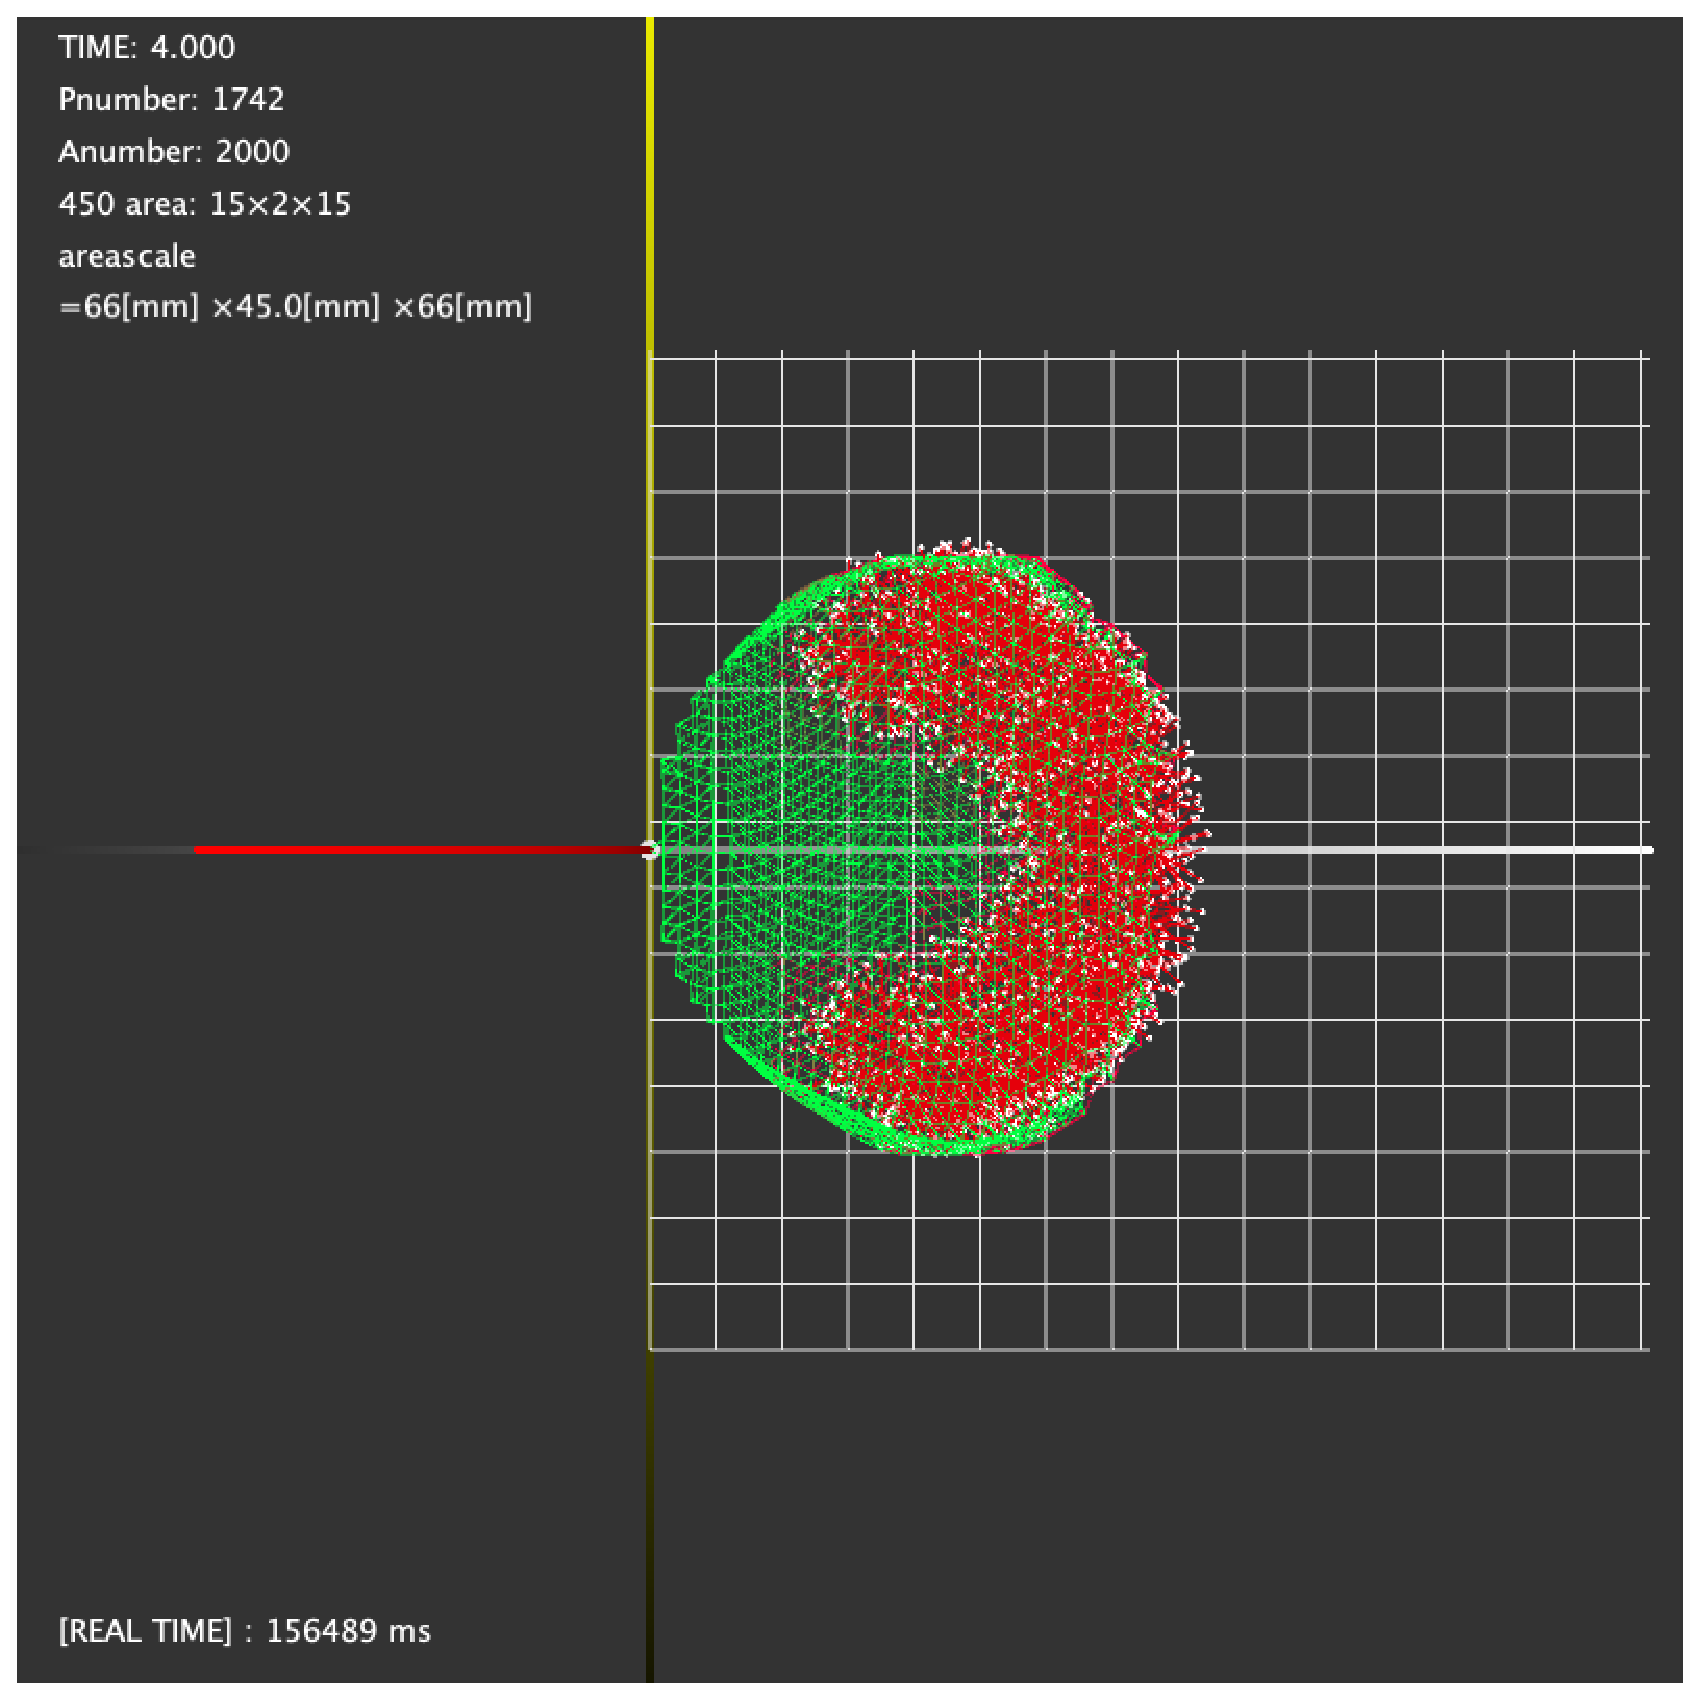
\includegraphics[width=5cm]{top40_arf.eps} \\
   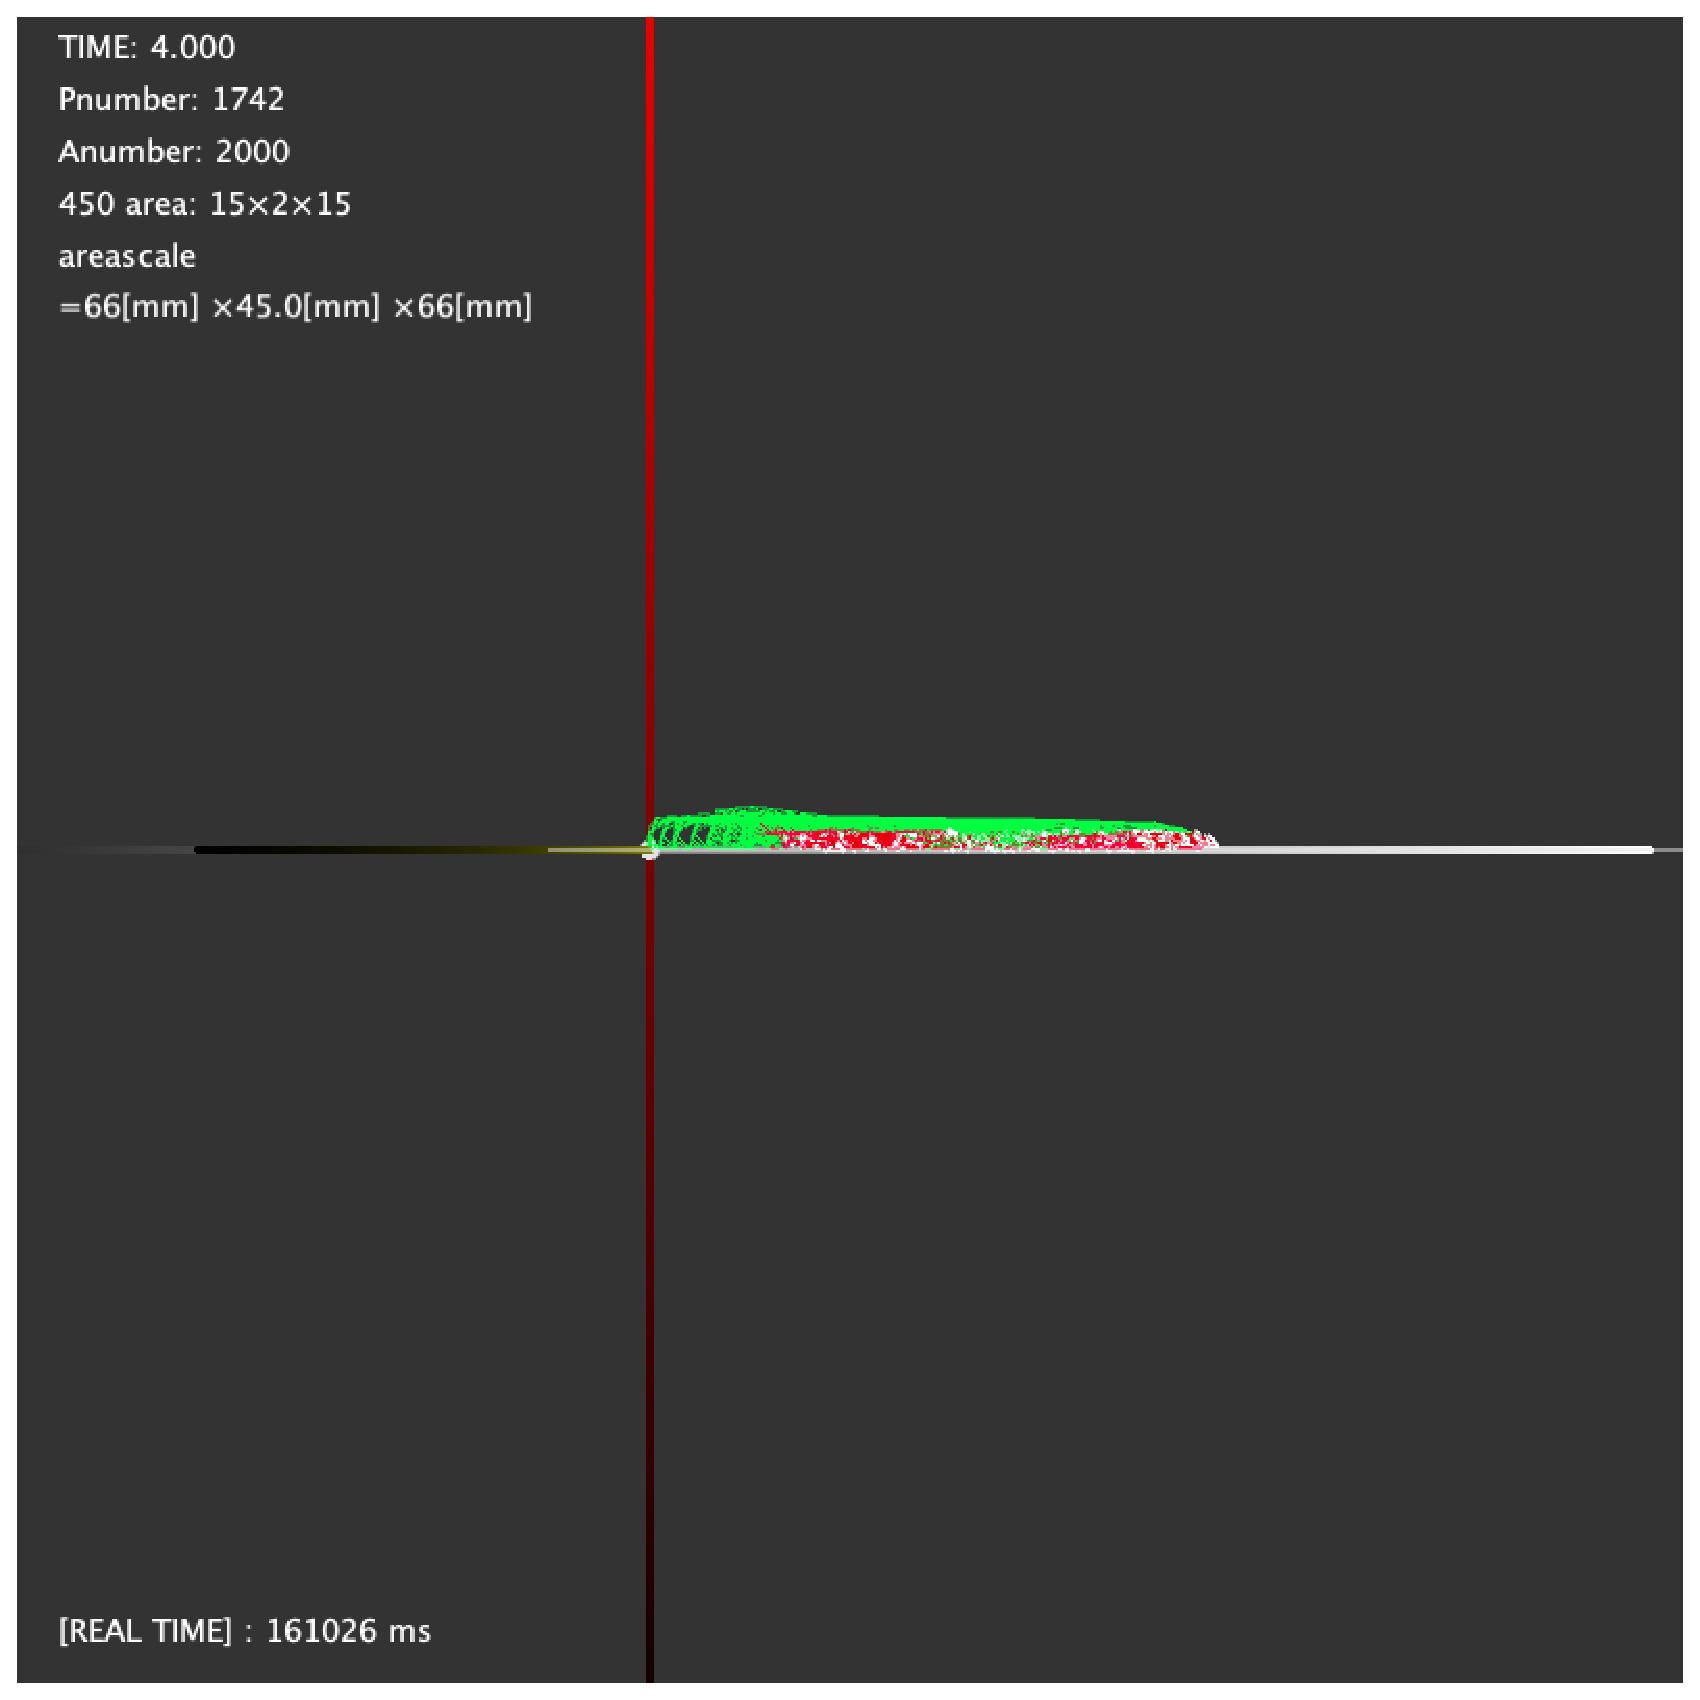
\includegraphics[width=5cm]{side40_arf.eps}
  \end{tabular}
 }%
 \caption{Simulation results. This is a picture of the keratocyte model taken at time $t = 0.5, 2.0, 4.0 [s]$. The top is the top view and the bottom is the side view pictures of the same time zone. A green line indicates a cell membrane, and a red dot indicates F-actin polymerized. Distance dependent ARF is used, and the setting value of relocation condition is 3.0\%.}
 \label{fig:res0}
\end{figure}

\begin{figure}[h]
 \subfloat[t=0.5.]{%
  \begin{tabular}{c}
   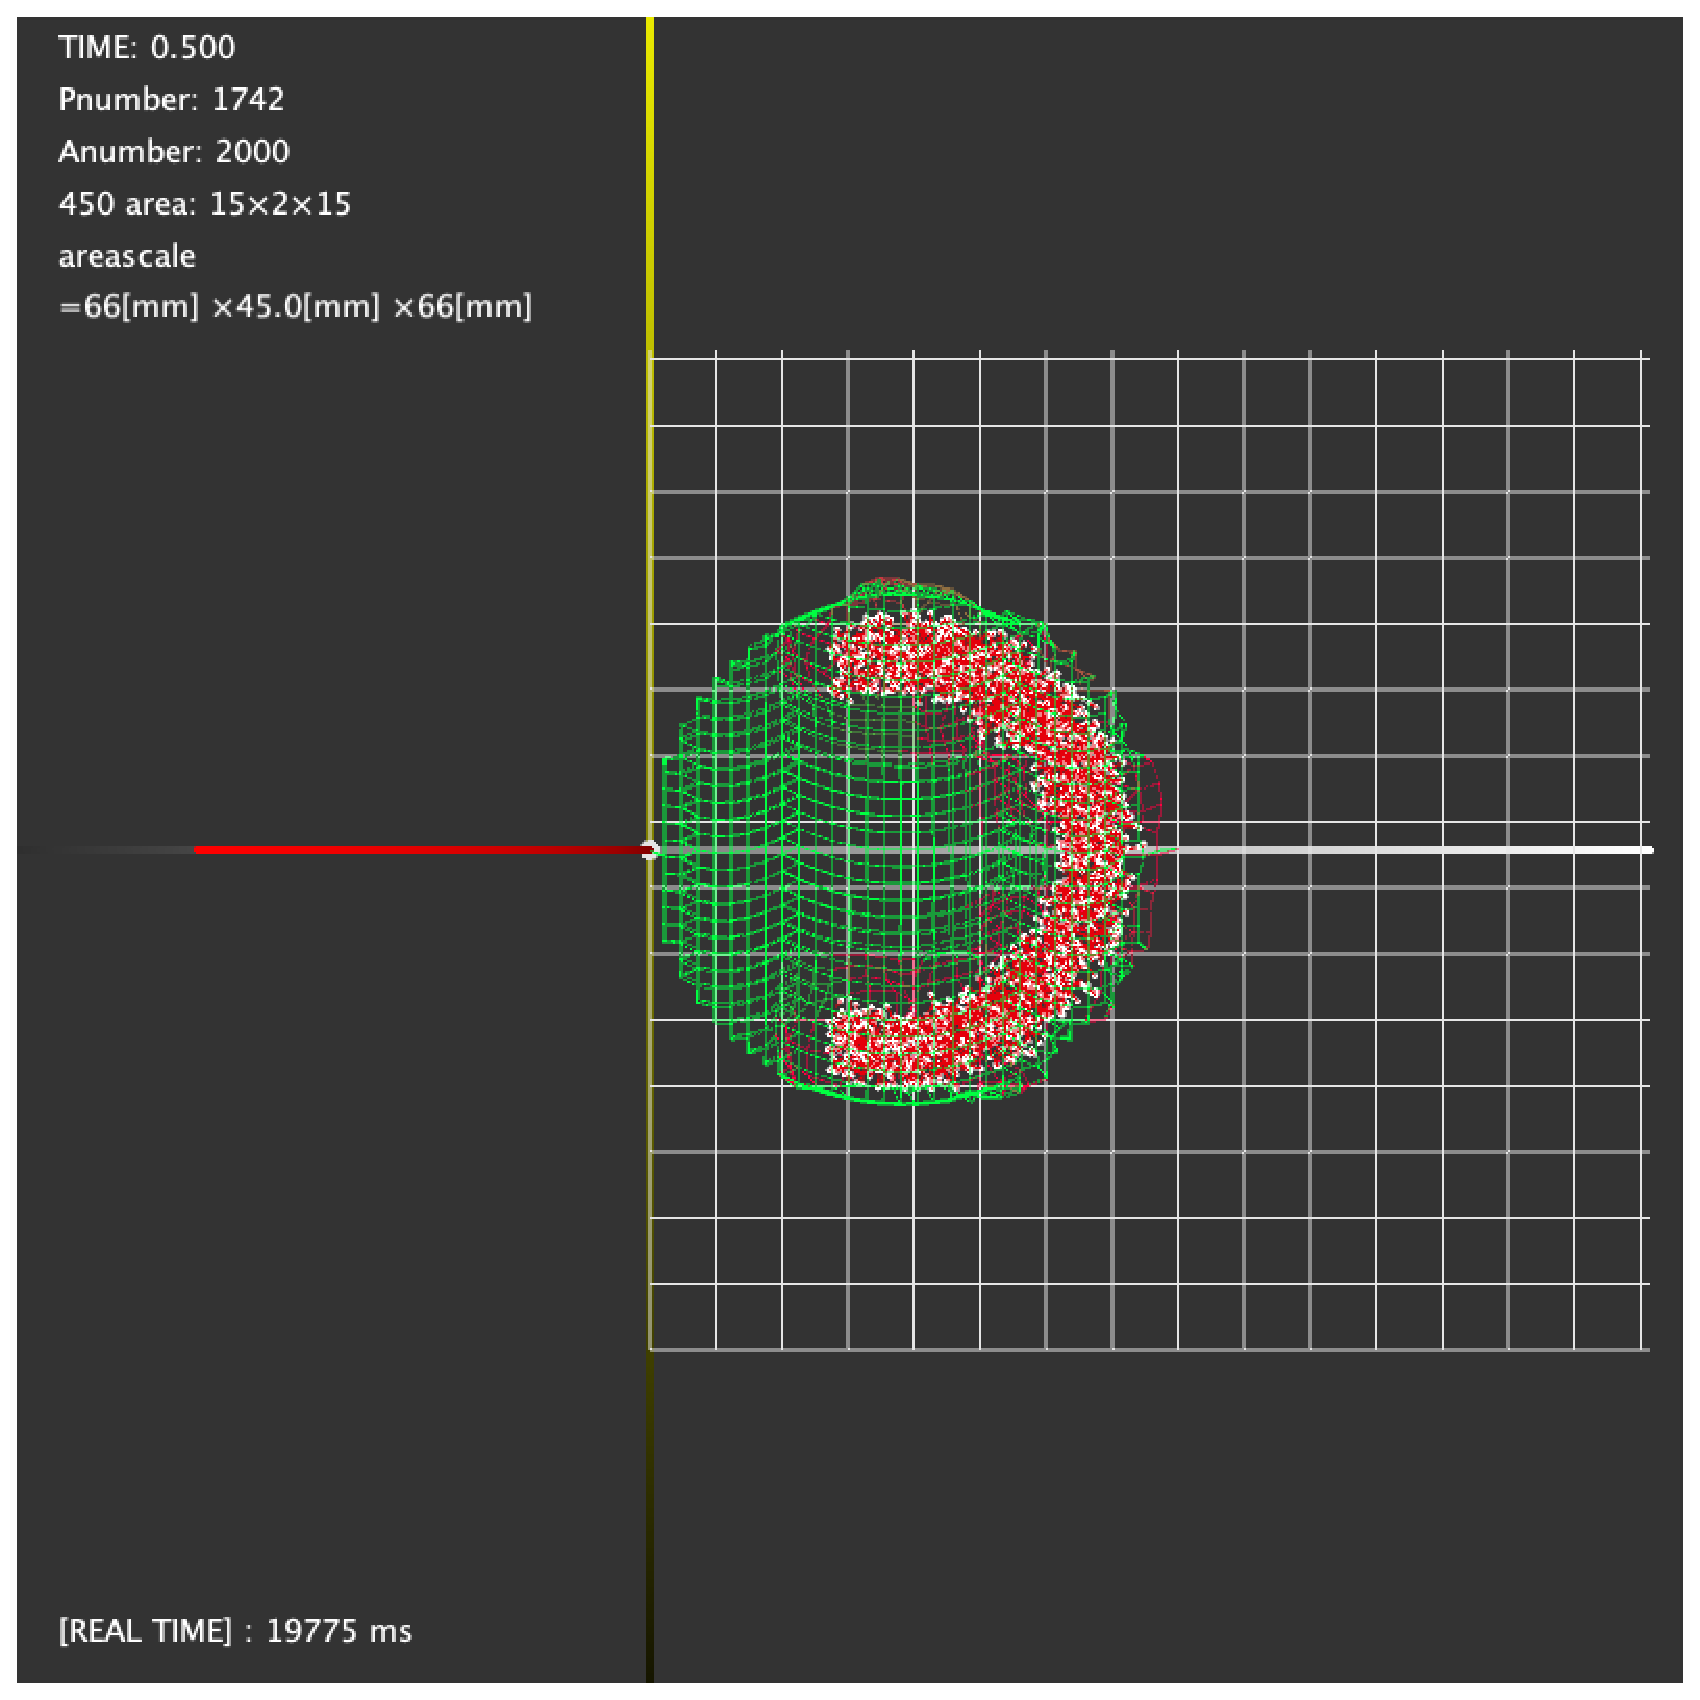
\includegraphics[width=5cm]{top05_iarf.eps} \\
   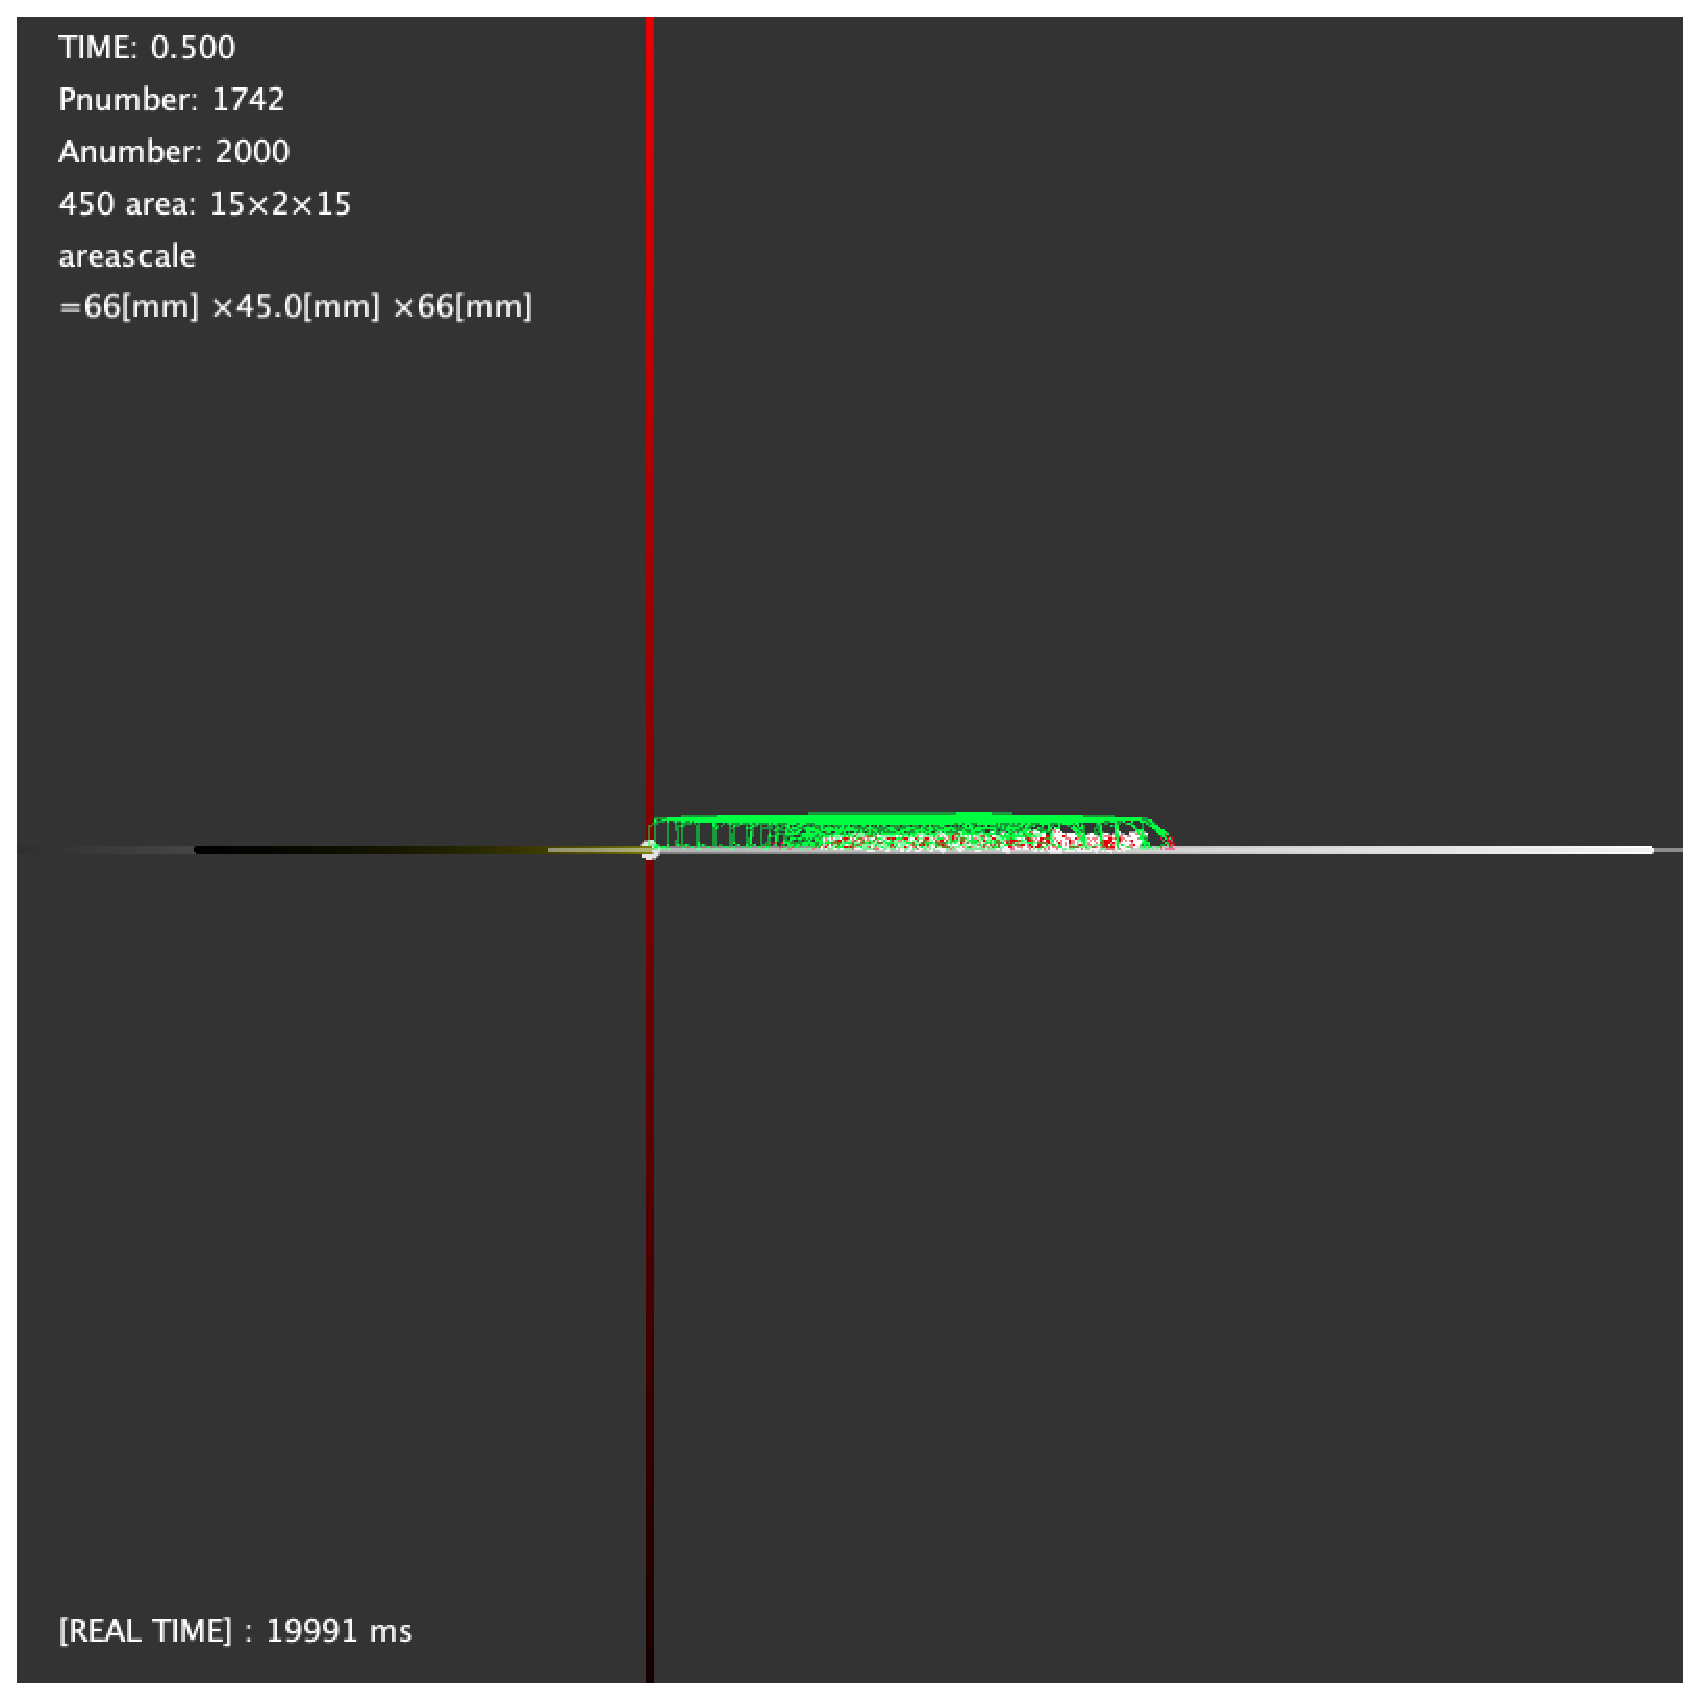
\includegraphics[width=5cm]{side05_iarf.eps}
  \end{tabular}
 }%
 \subfloat[t=2.0]{%
  \begin{tabular}{c}
   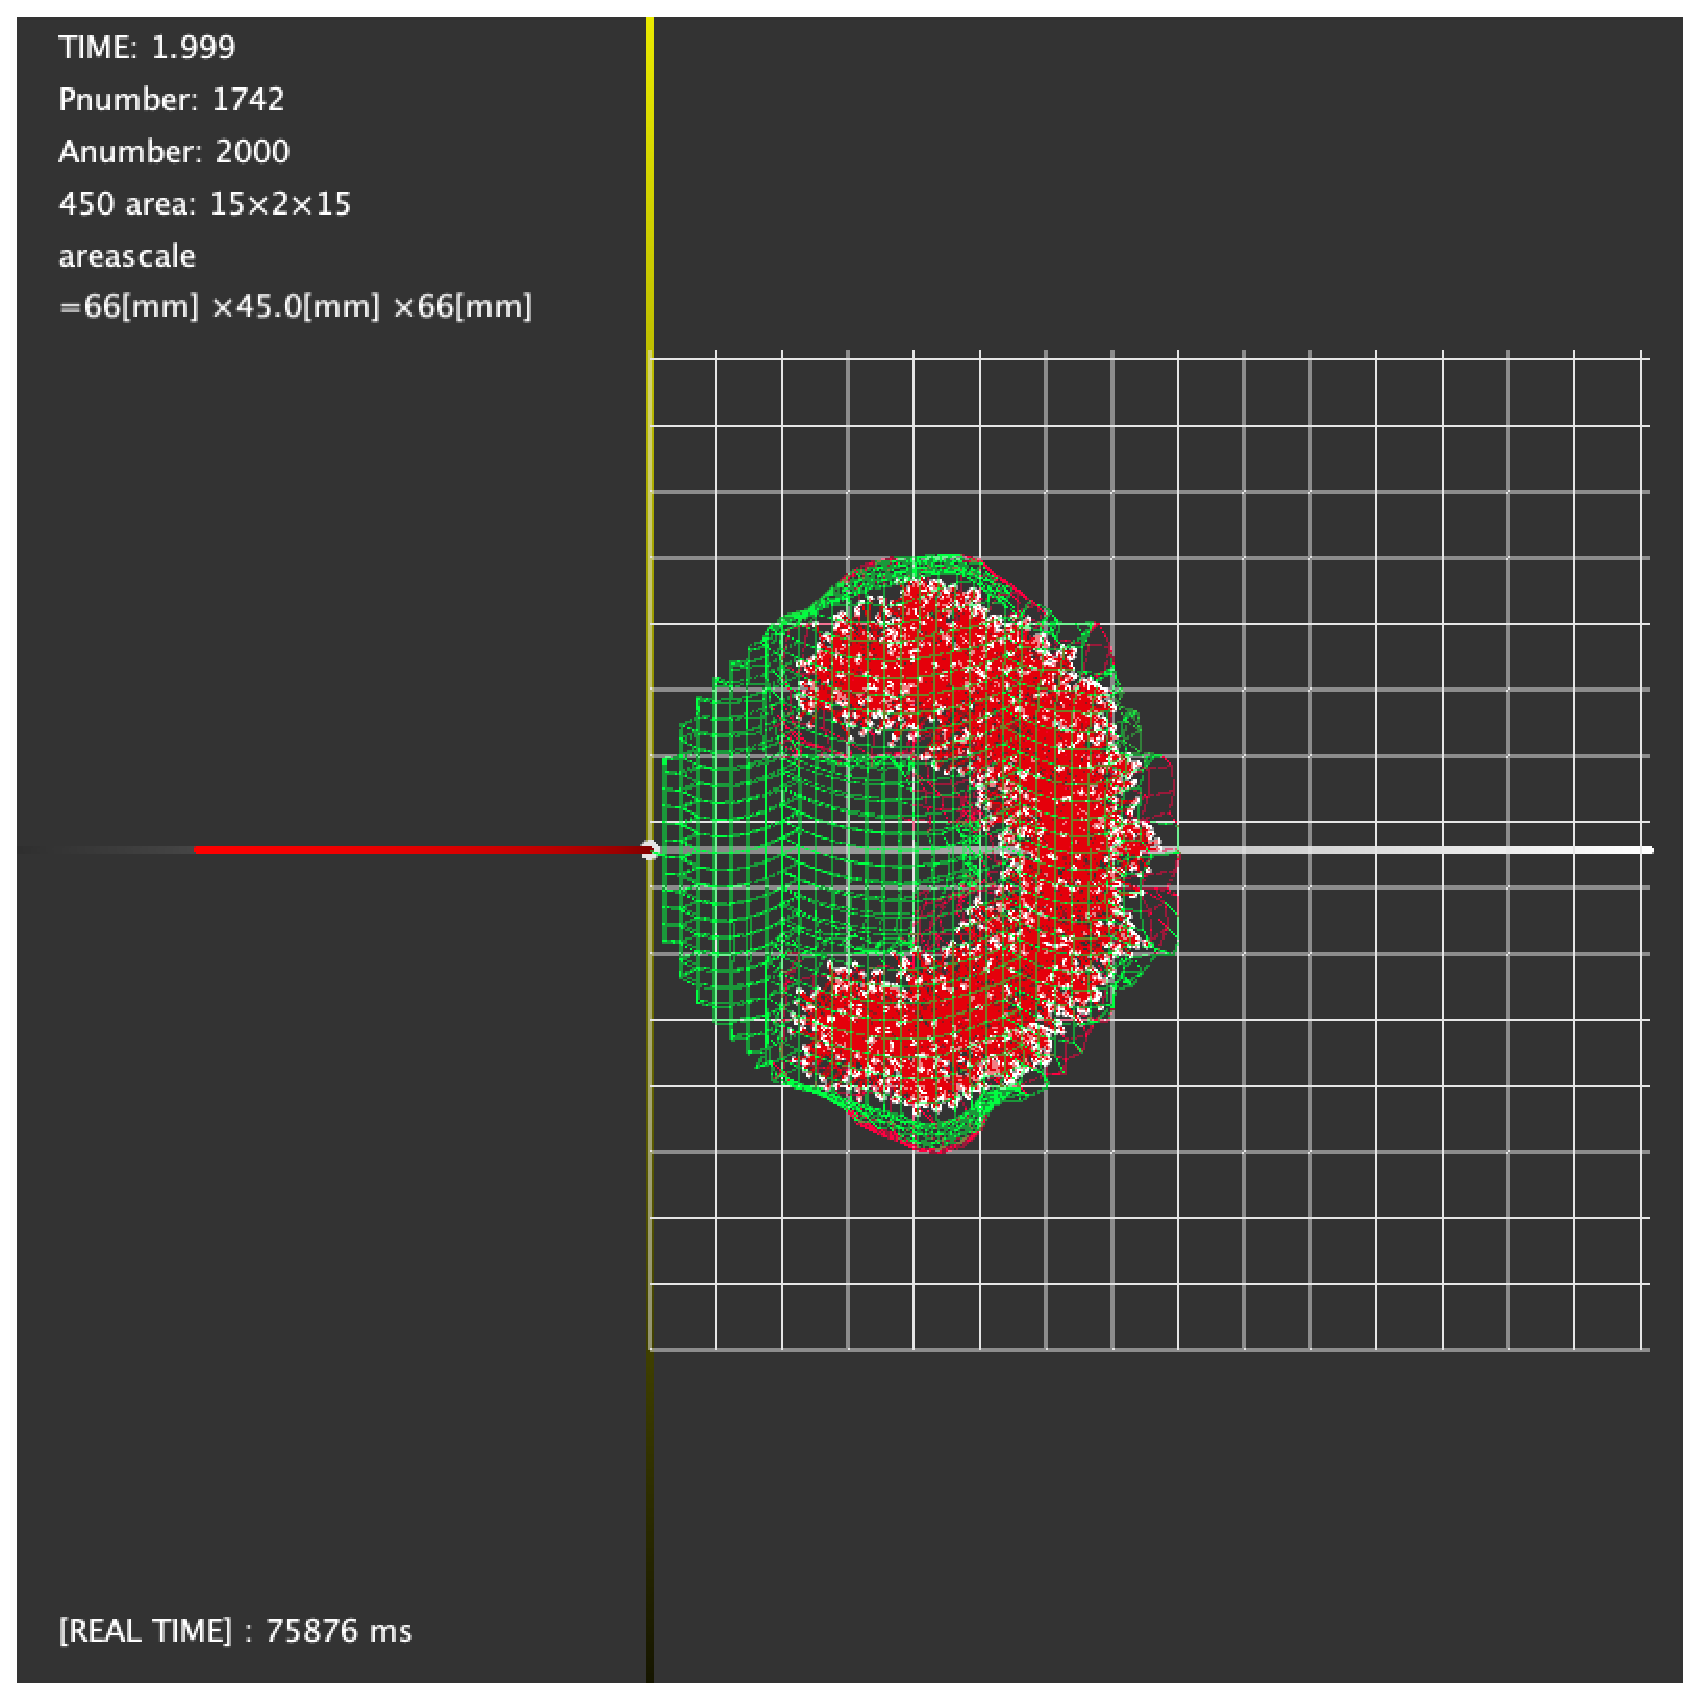
\includegraphics[width=5cm]{top20_iarf.eps} \\
   \includegraphics[width=5cm]{side20_iarf.eps}
  \end{tabular}
 }%
 \subfloat[t=4.0]{%
  \begin{tabular}{c}
   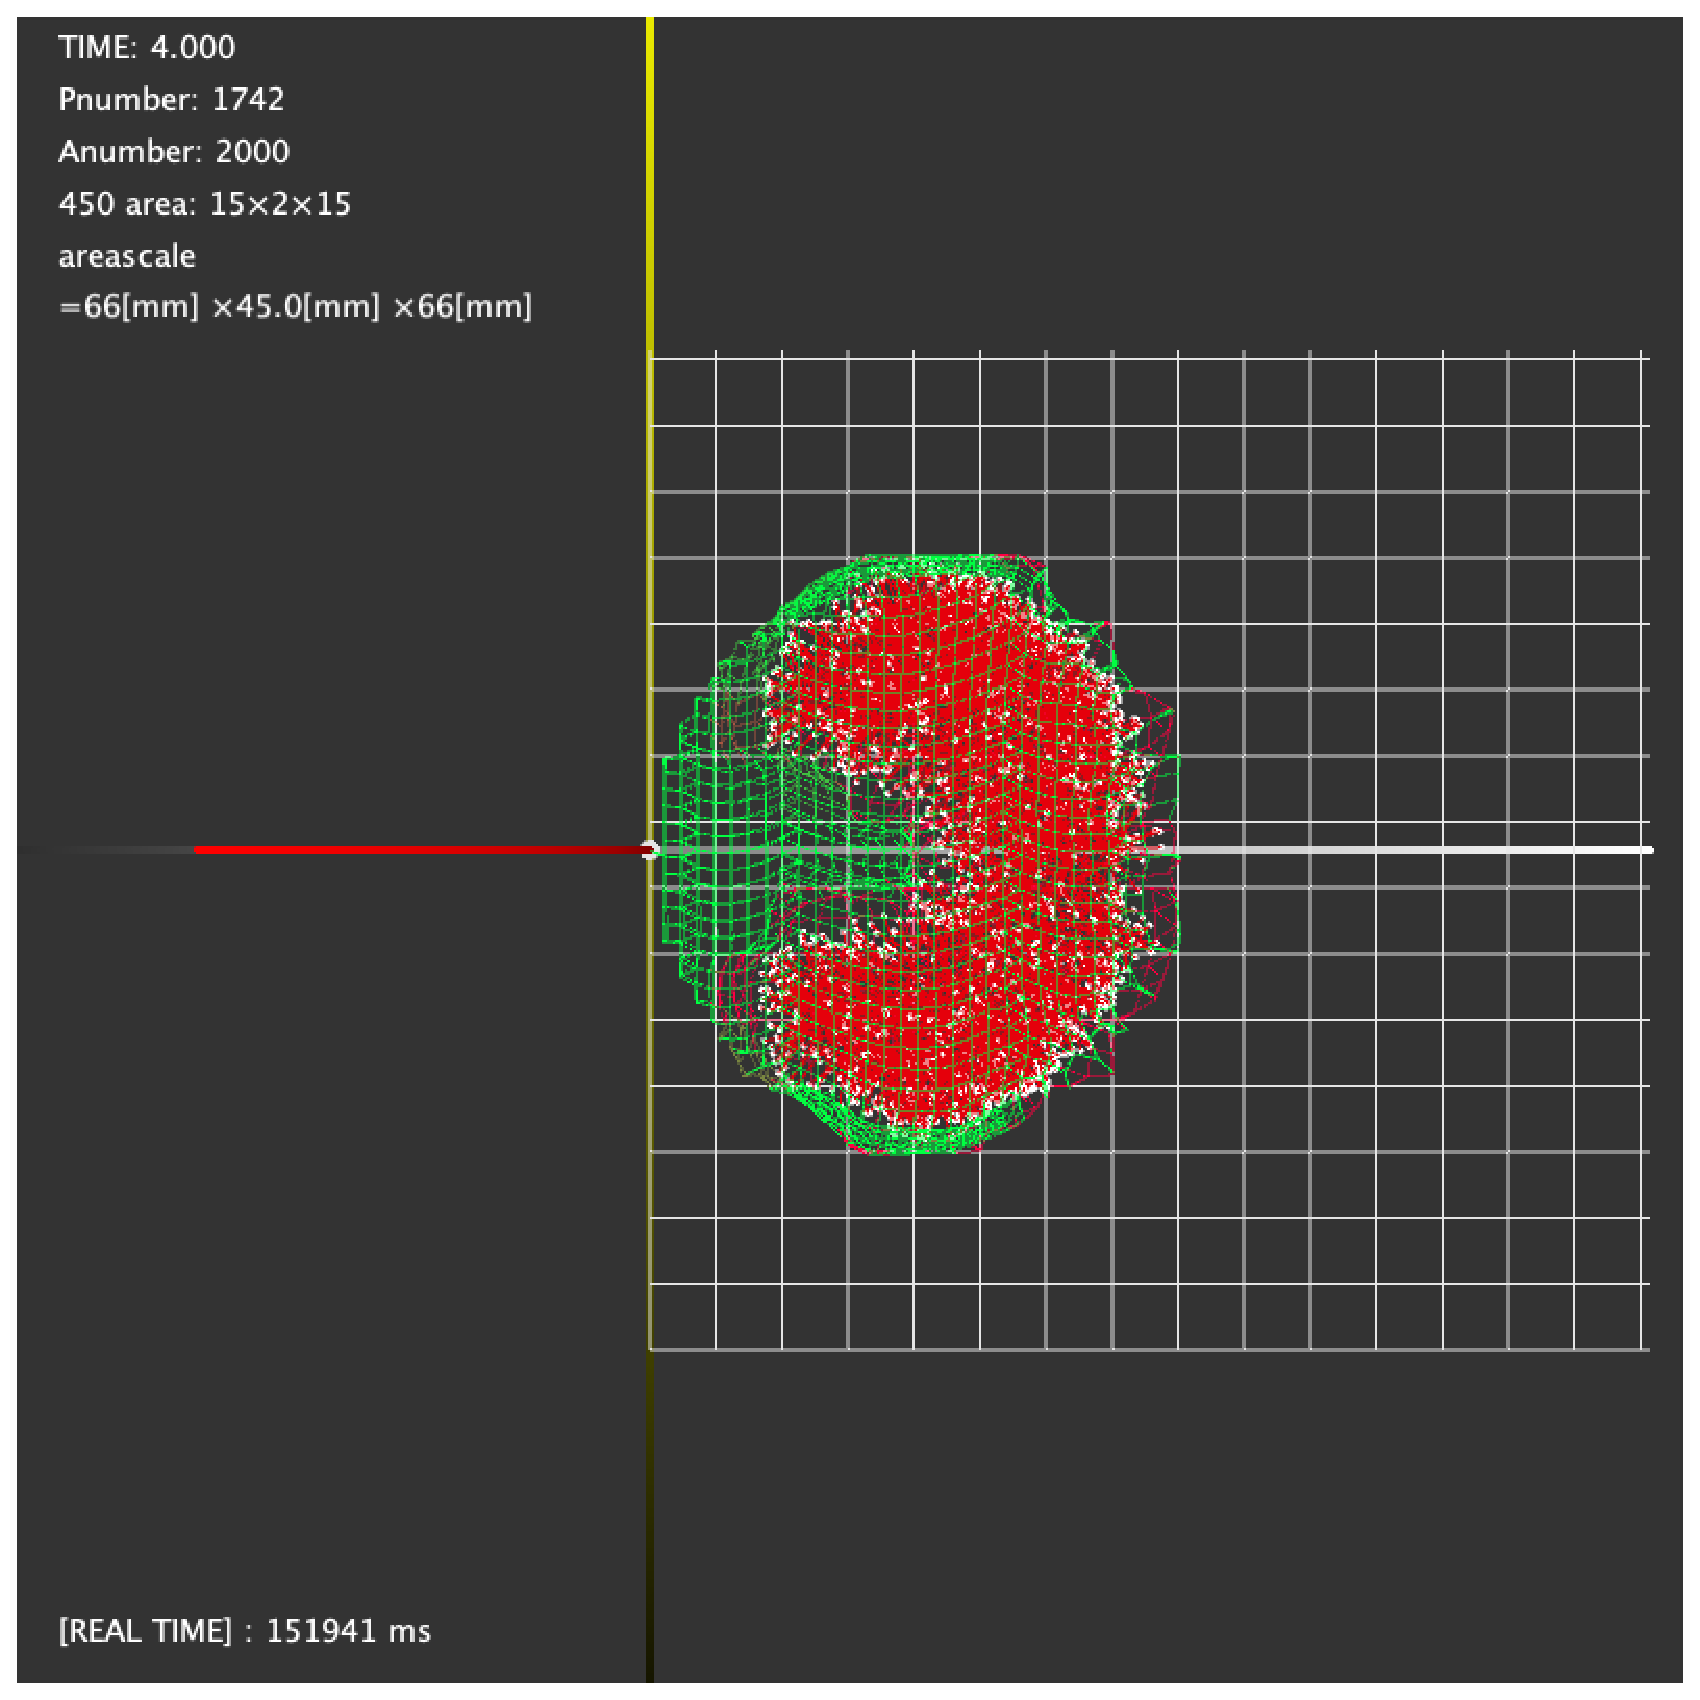
\includegraphics[width=5cm]{top40_iarf.eps} \\
   \includegraphics[width=5cm]{side40_iarf.eps}
  \end{tabular}
 }%
 \caption{Simulation results for distance independent ARF.}
 \label{fig:res1}
\end{figure}

\begin{figure}[h]
 \subfloat[t=0.5.]{%
  \begin{tabular}{c}
   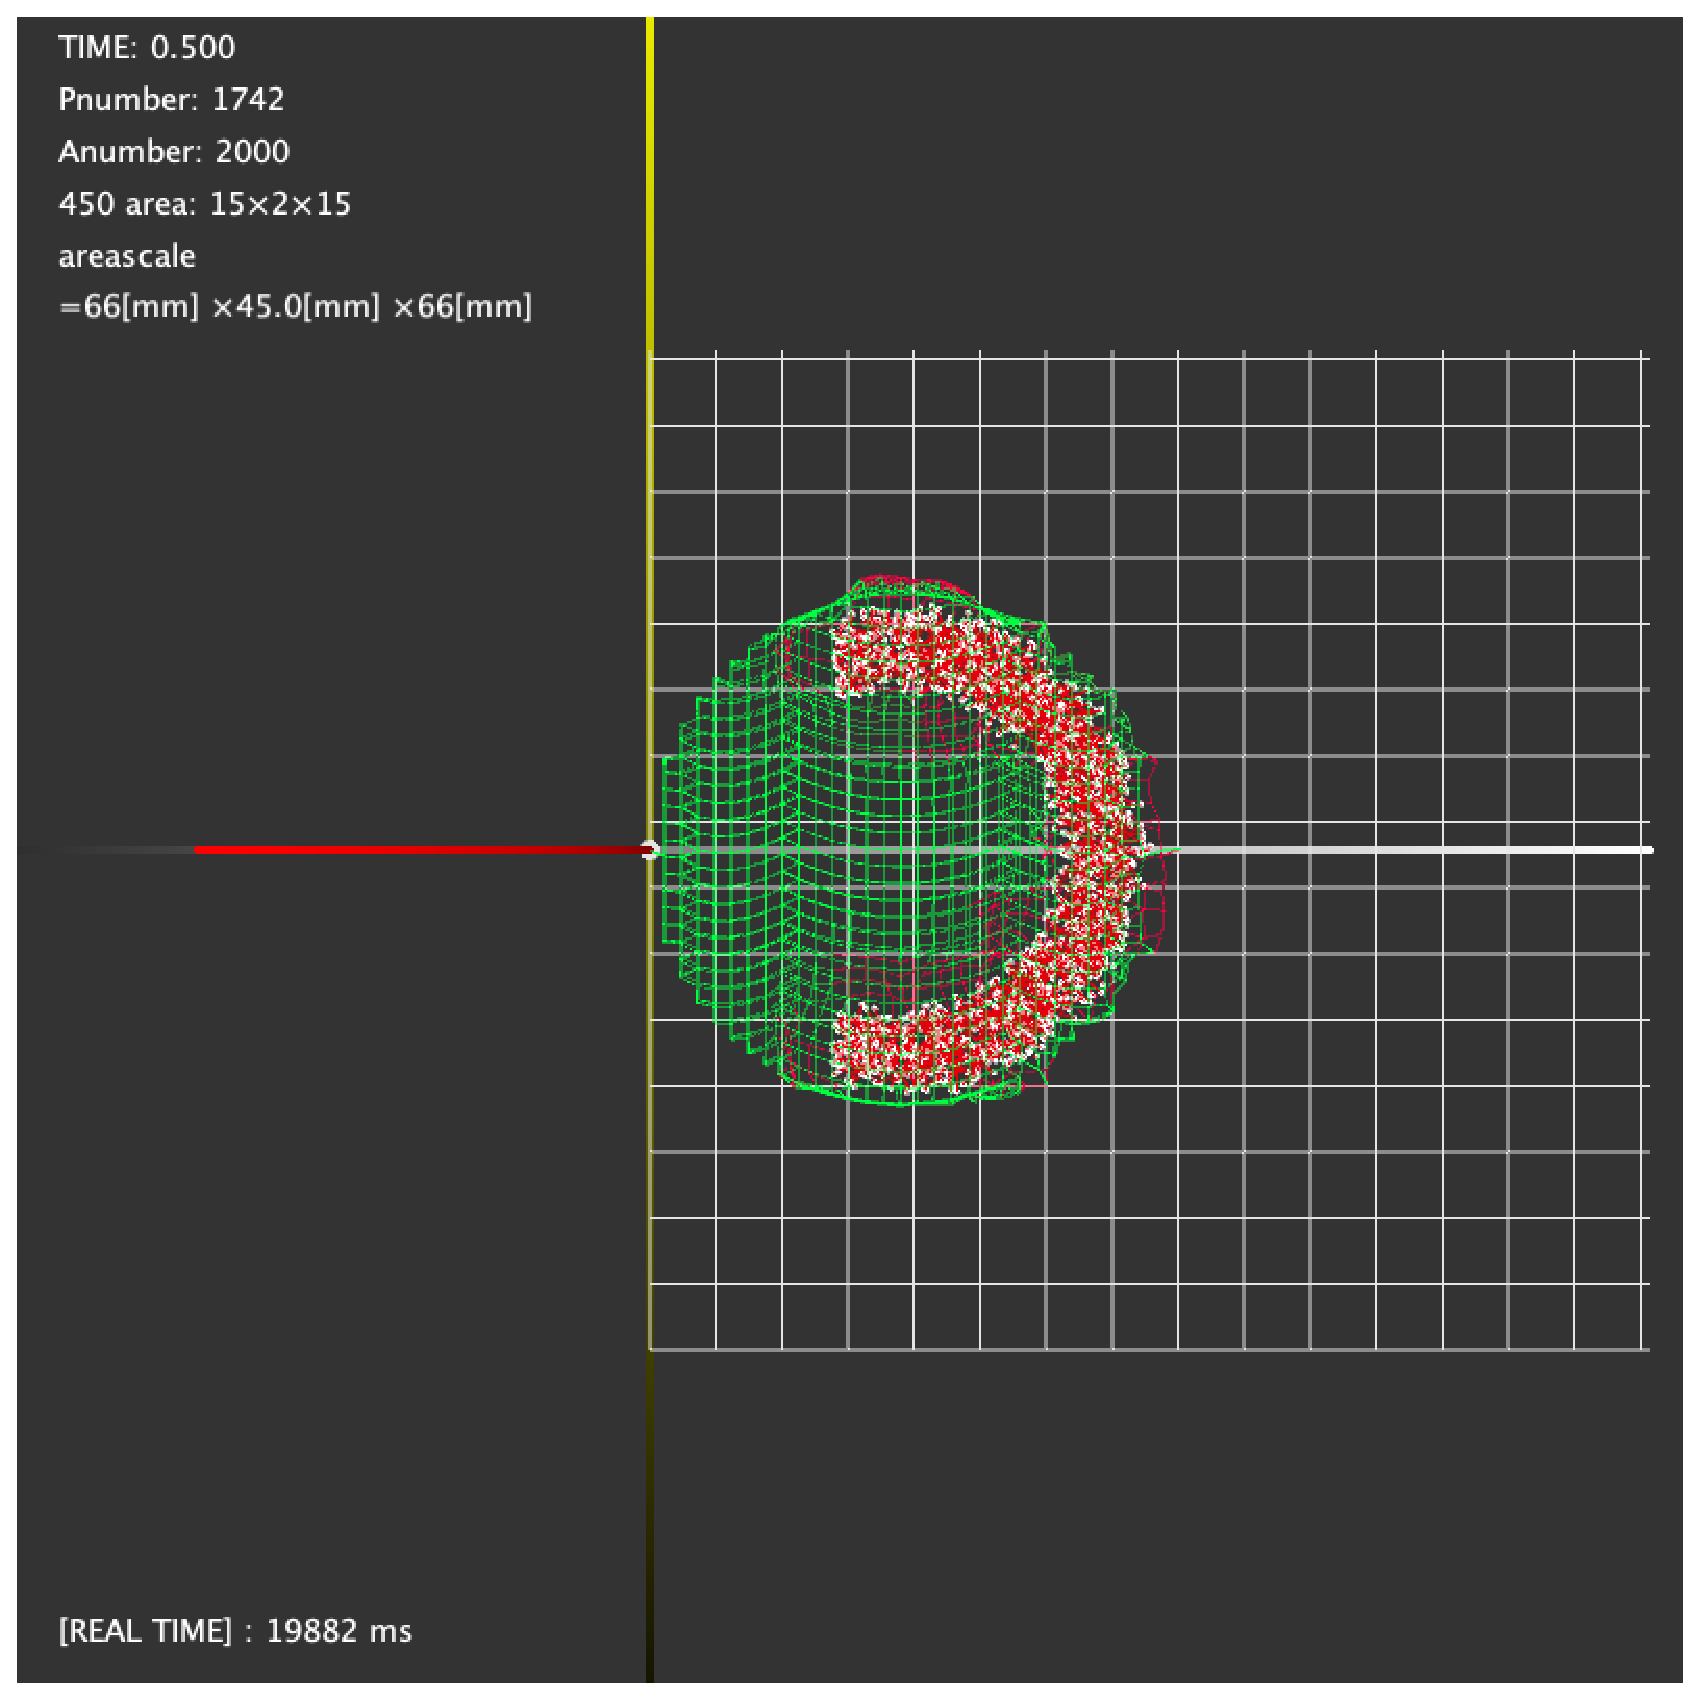
\includegraphics[width=5cm]{top05_narf.eps} \\
   \includegraphics[width=5cm]{side05_narf.eps}
  \end{tabular}
 }%
 \subfloat[t=2.0]{%
  \begin{tabular}{c}
   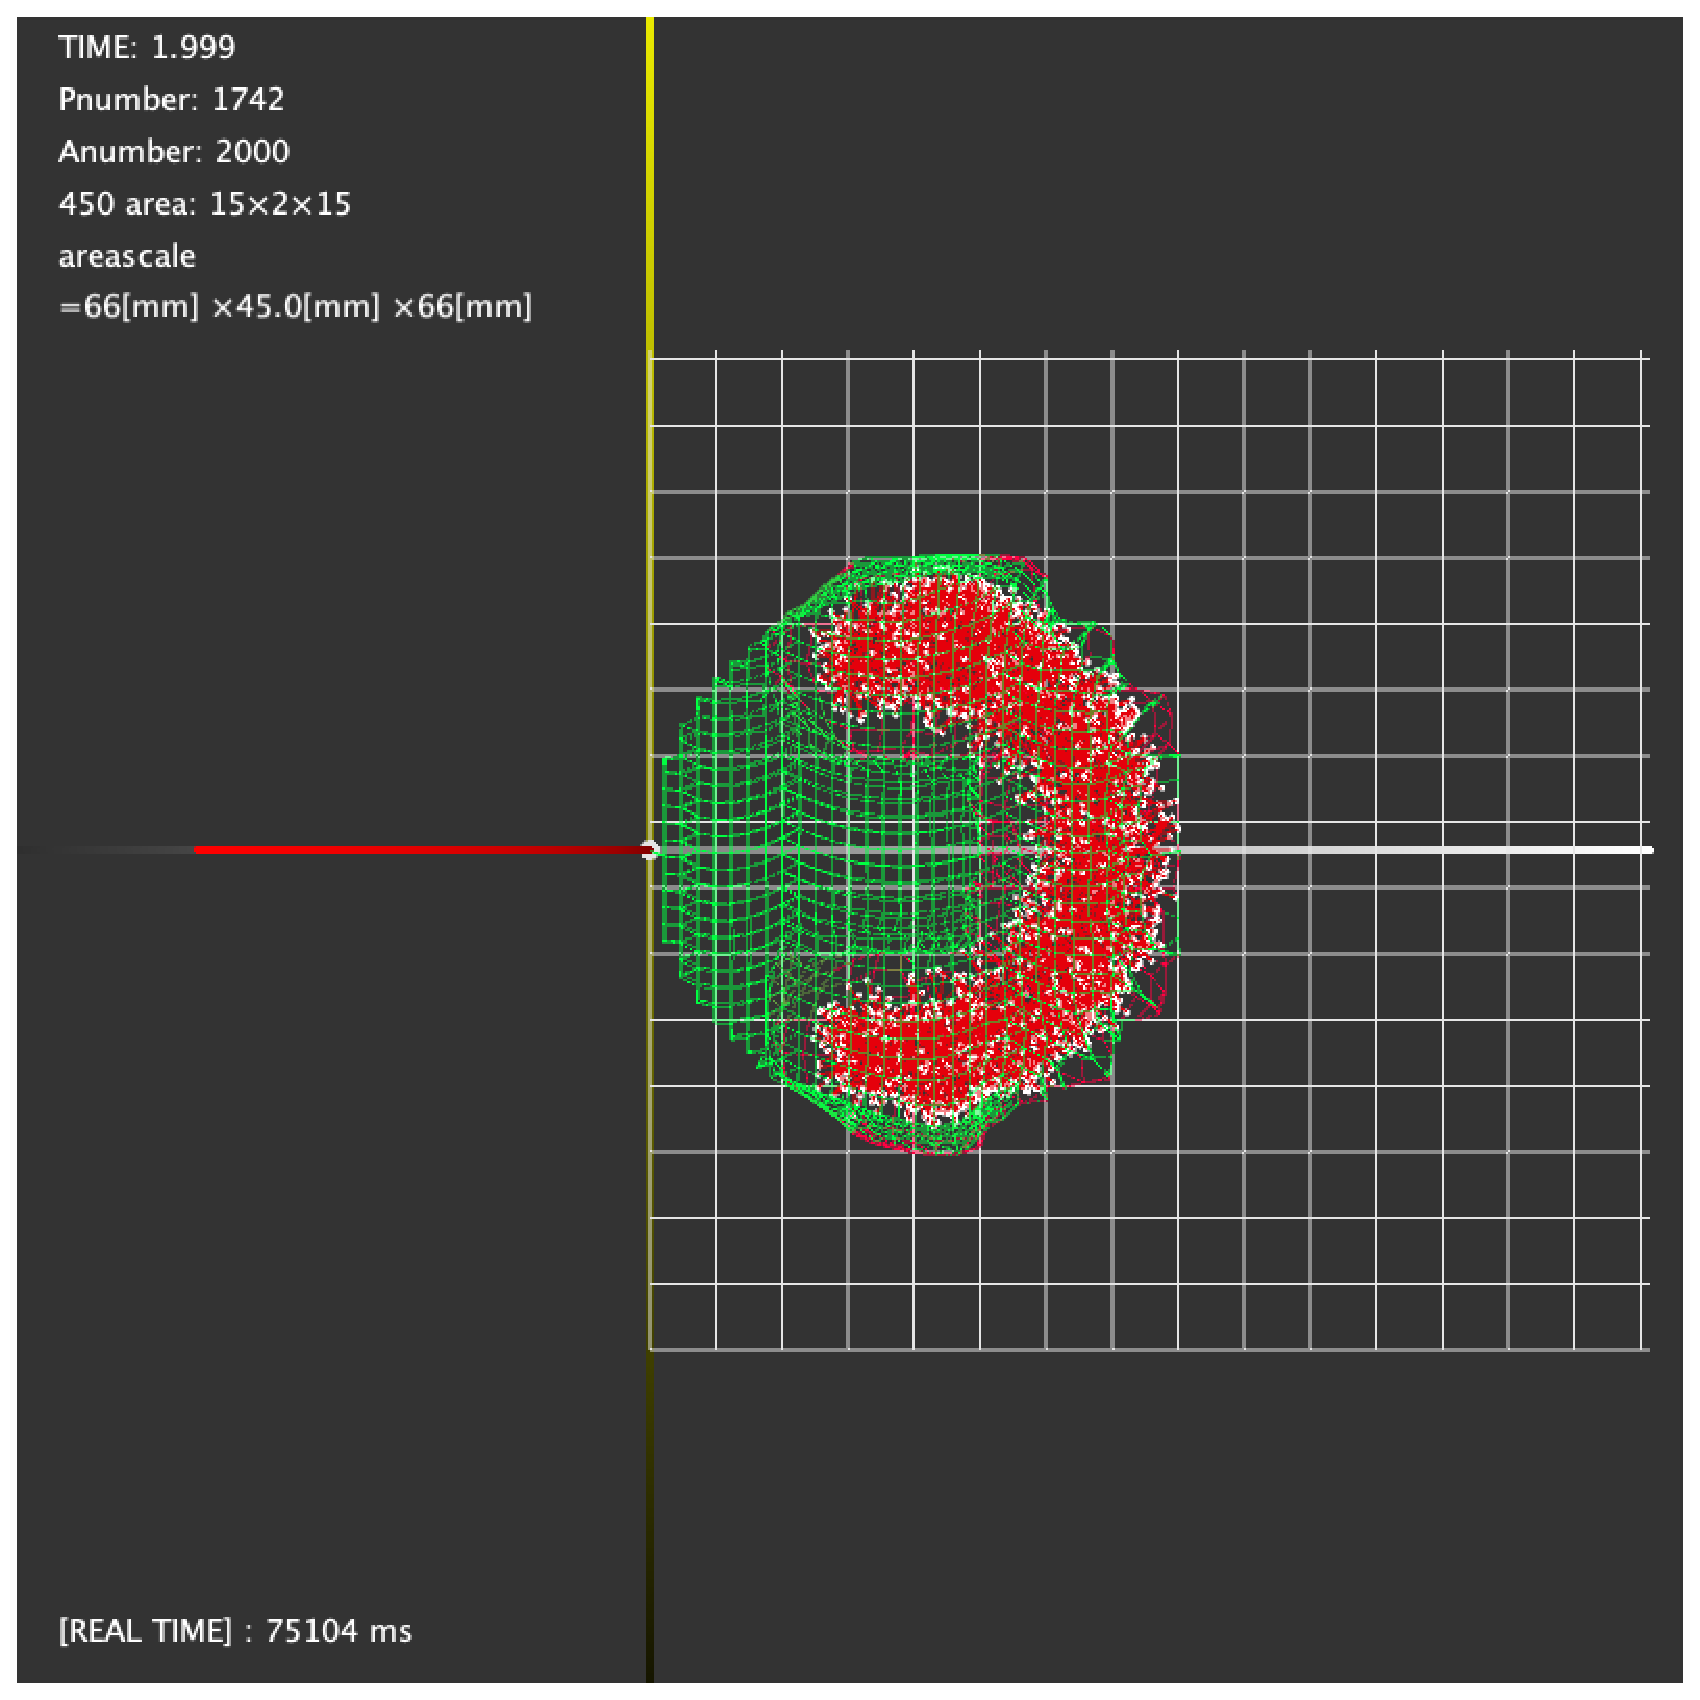
\includegraphics[width=5cm]{top20_narf.eps} \\
   \includegraphics[width=5cm]{side20_narf.eps}
  \end{tabular}
 }%
 \subfloat[t=4.0]{%
  \begin{tabular}{c}
   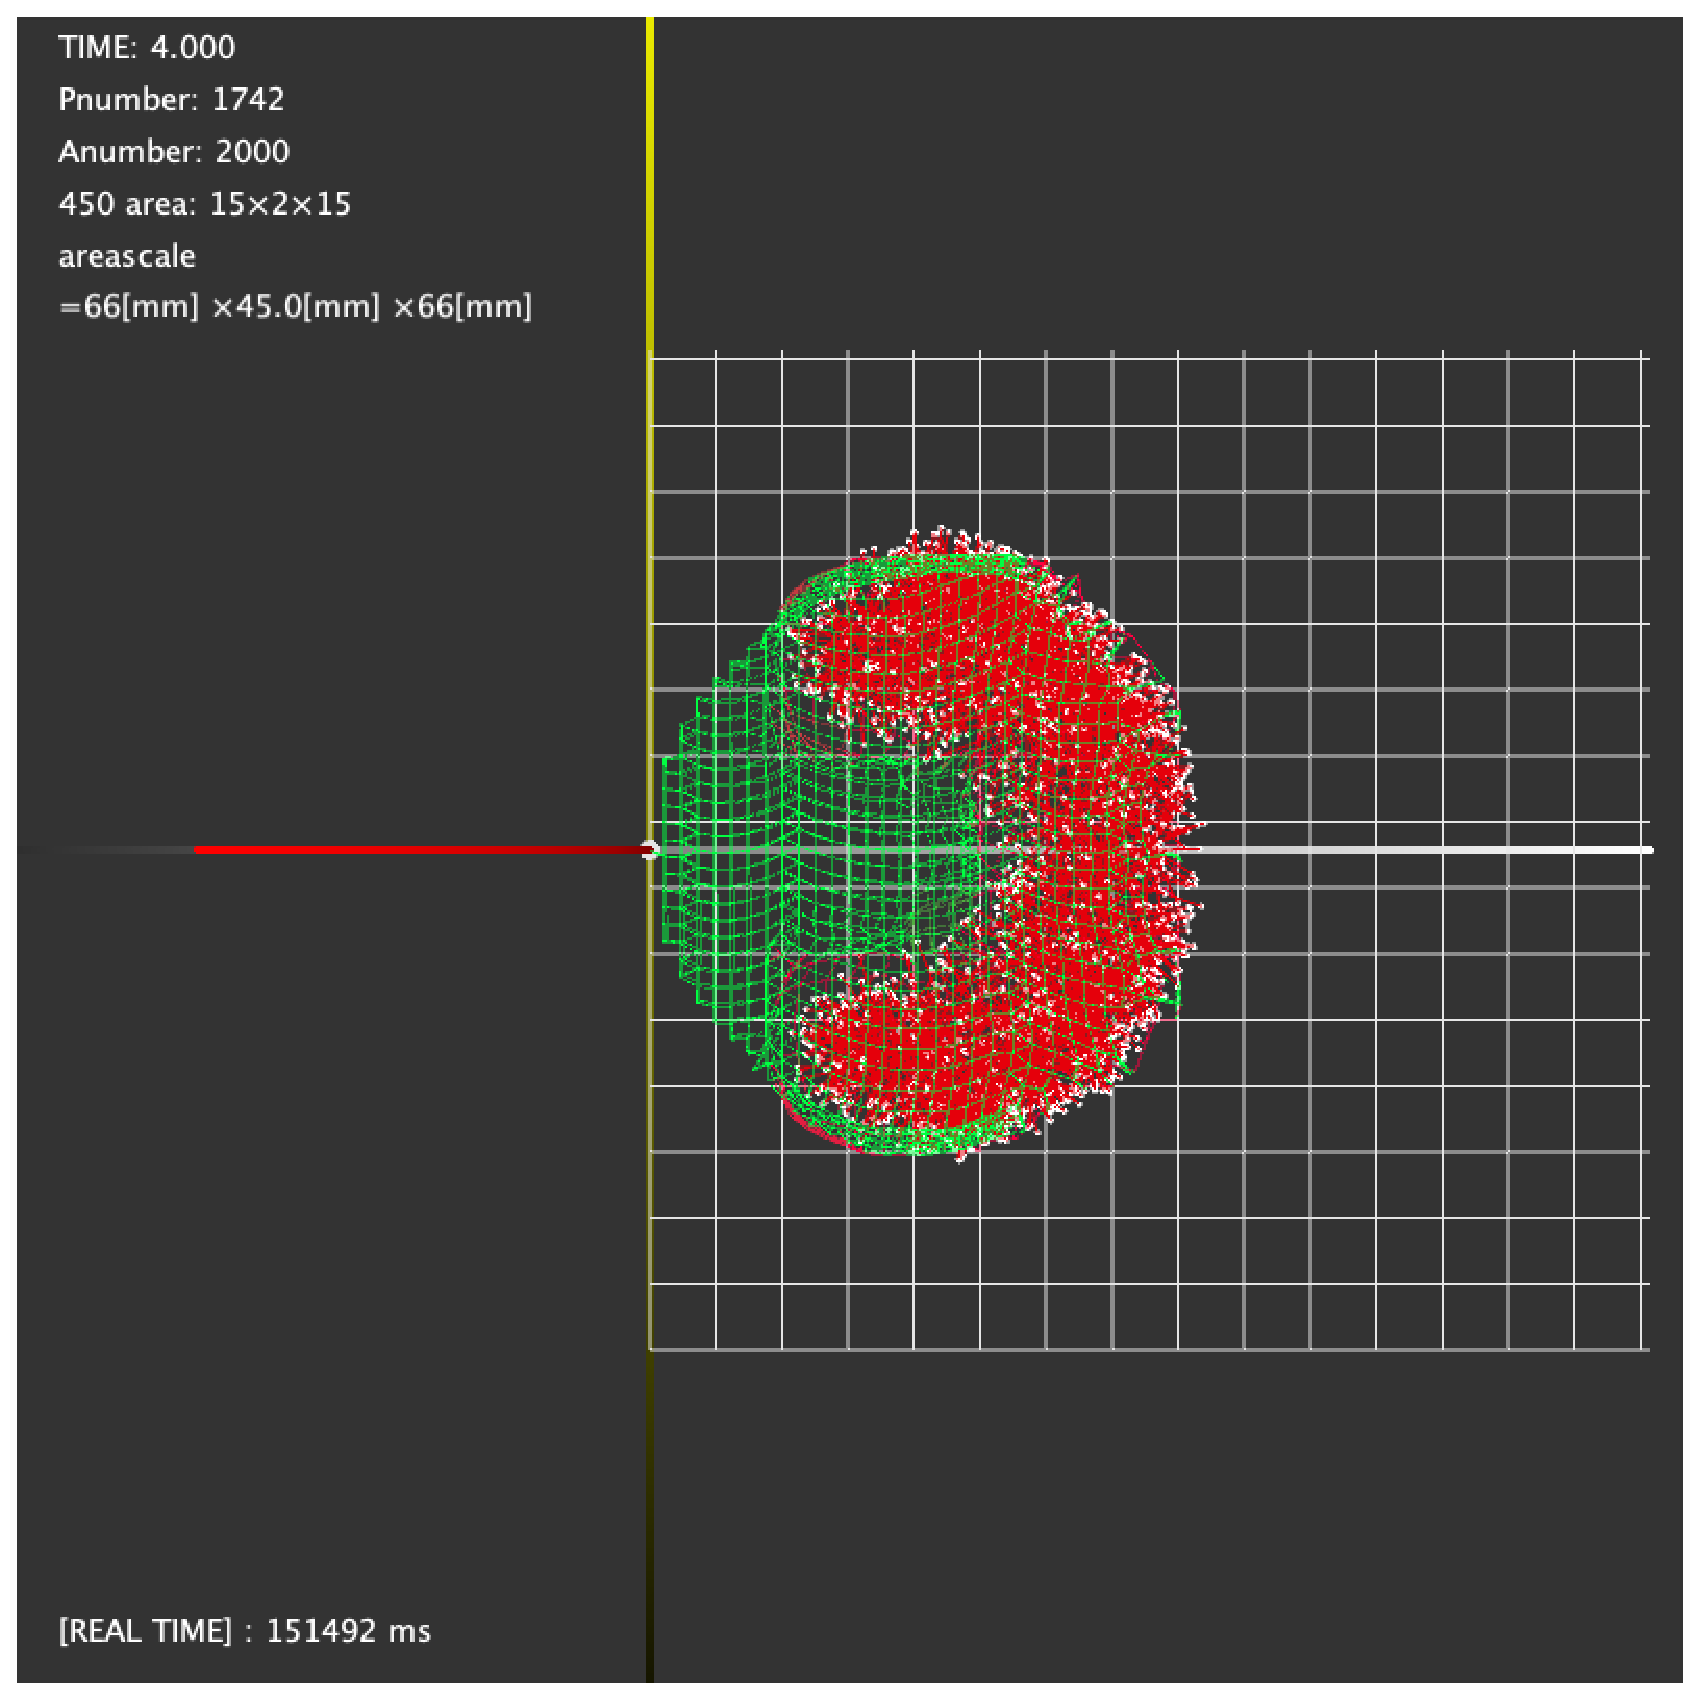
\includegraphics[width=5cm]{top40_narf.eps} \\
   \includegraphics[width=5cm]{side40_narf.eps}
  \end{tabular}
 }%
 \caption{Simulation Results without ARF.}
 \label{fig:res2}
\end{figure}

Experiments were carried out by distinguishing the ARF according to the distance from the distance between the actin molecule and the reference point $\bm{E}$ and the ARF which is distance independent. The results of simulation experiments are shown in Fig \ref{fig:res0}. Actin polymerization progressed as the time progressed, and the cell membrane was compressed. The cell membrane deformed reflecting the action of force from the inside. However, it was only in the region of cell membrane progression direction, the opposite side stuck to the substrate. There was a flaw in this simulation concerning deformation of the cell membrane. Regarding the actin molecule which is the cytoskeleton, it is successfully formed in a crescent shape, but the cell membrane in the posterior portion has not moved.

\subsection{Position of Actin retrograde flow reference point}
\begin{figure}[h]
 \subfloat[t=0.5.]{%
  \begin{tabular}{c}
   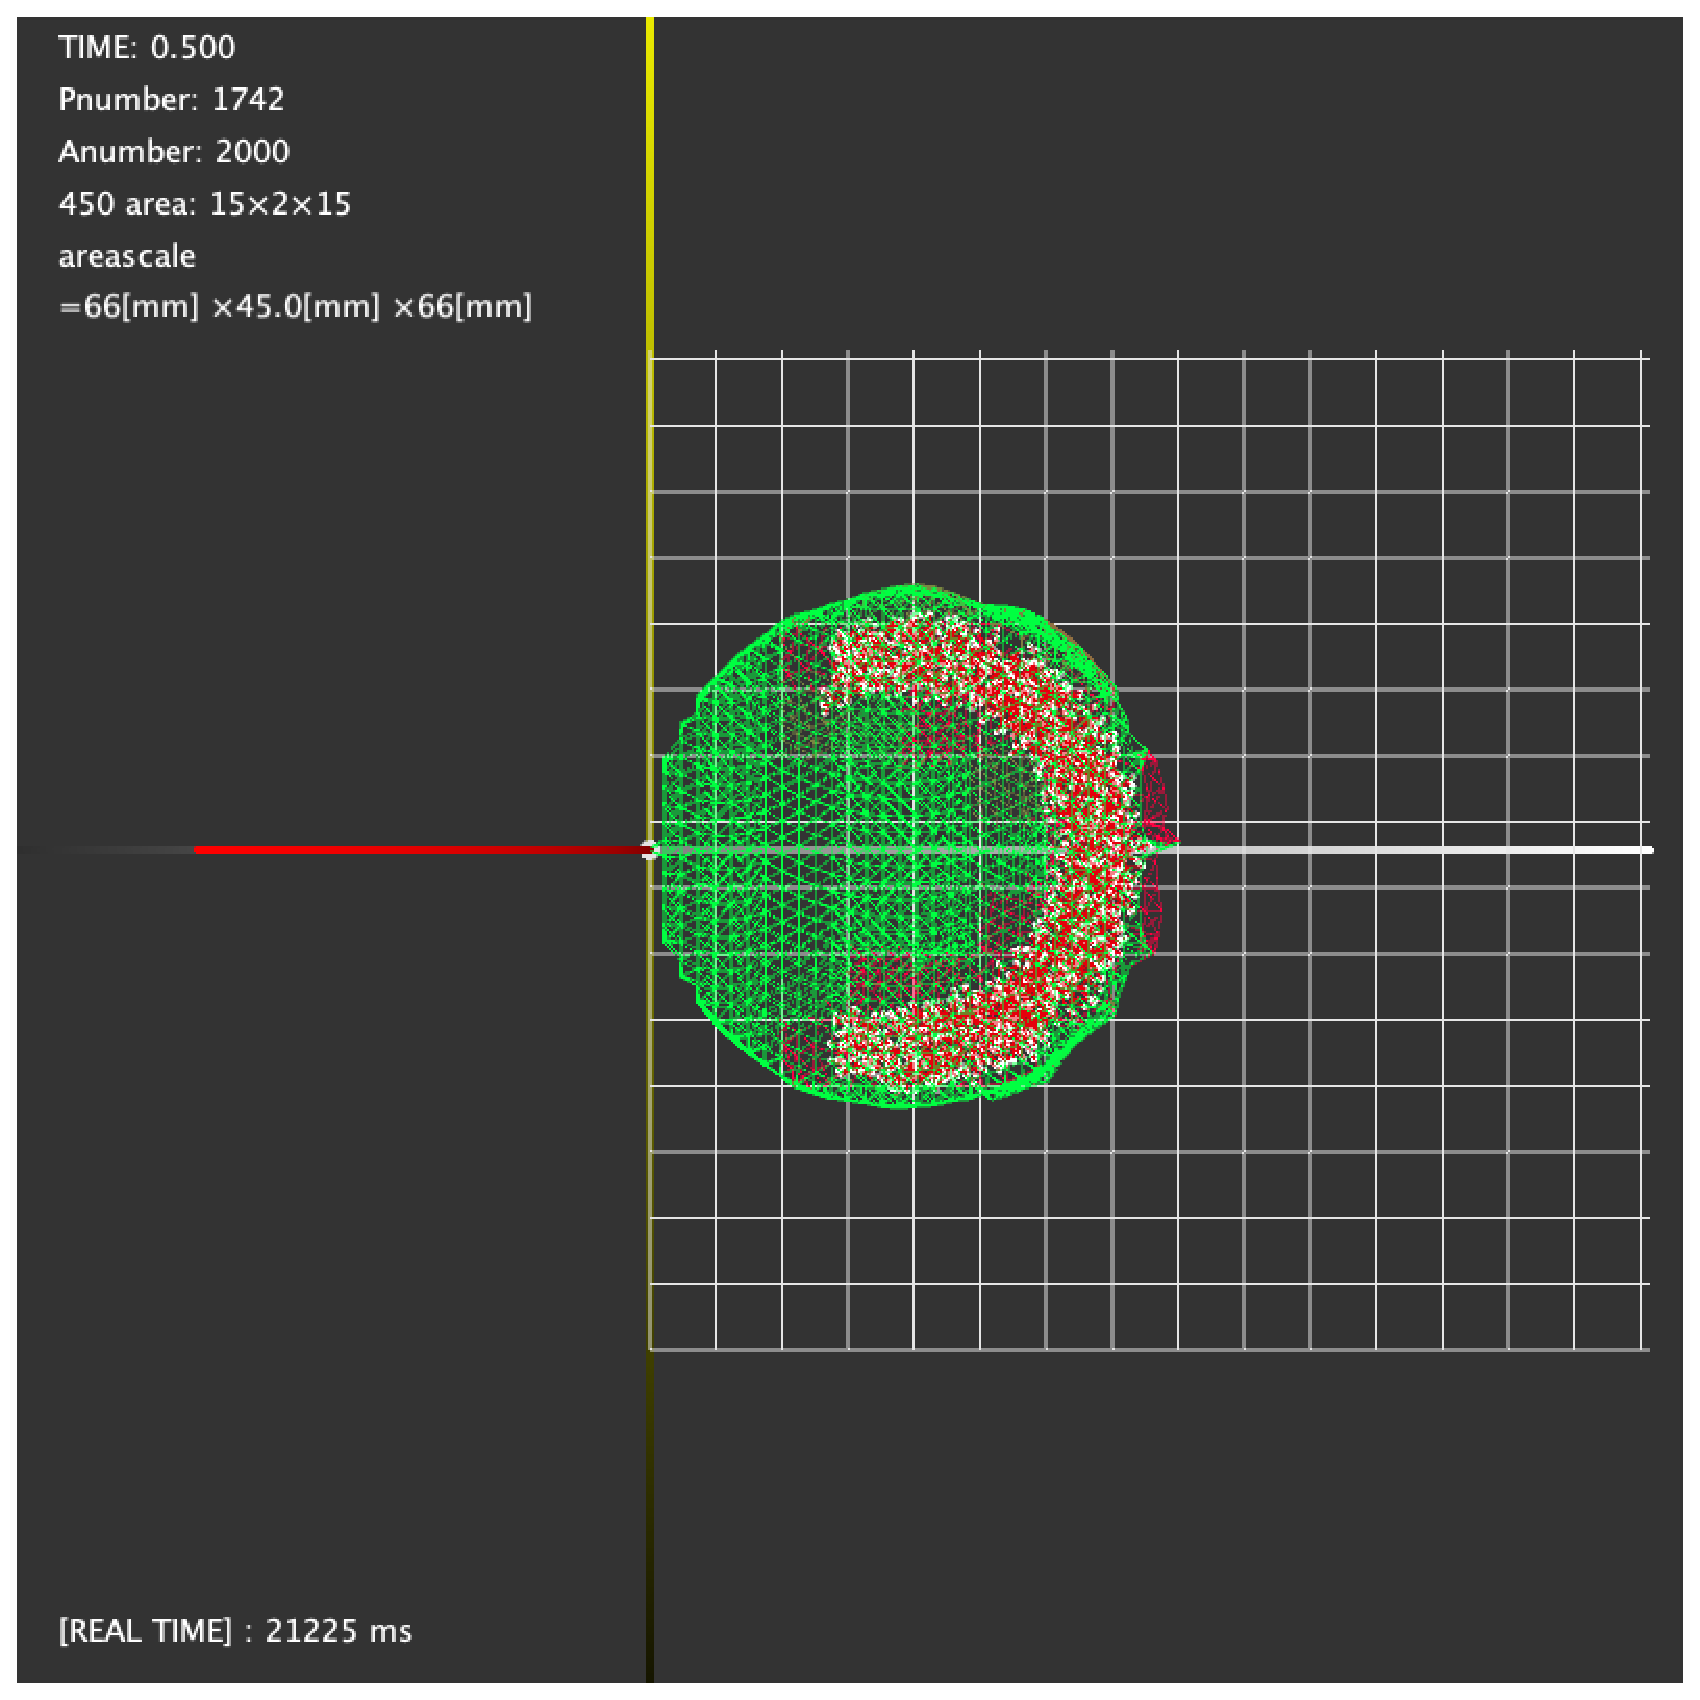
\includegraphics[width=5cm]{top05_2arf.eps} \\
   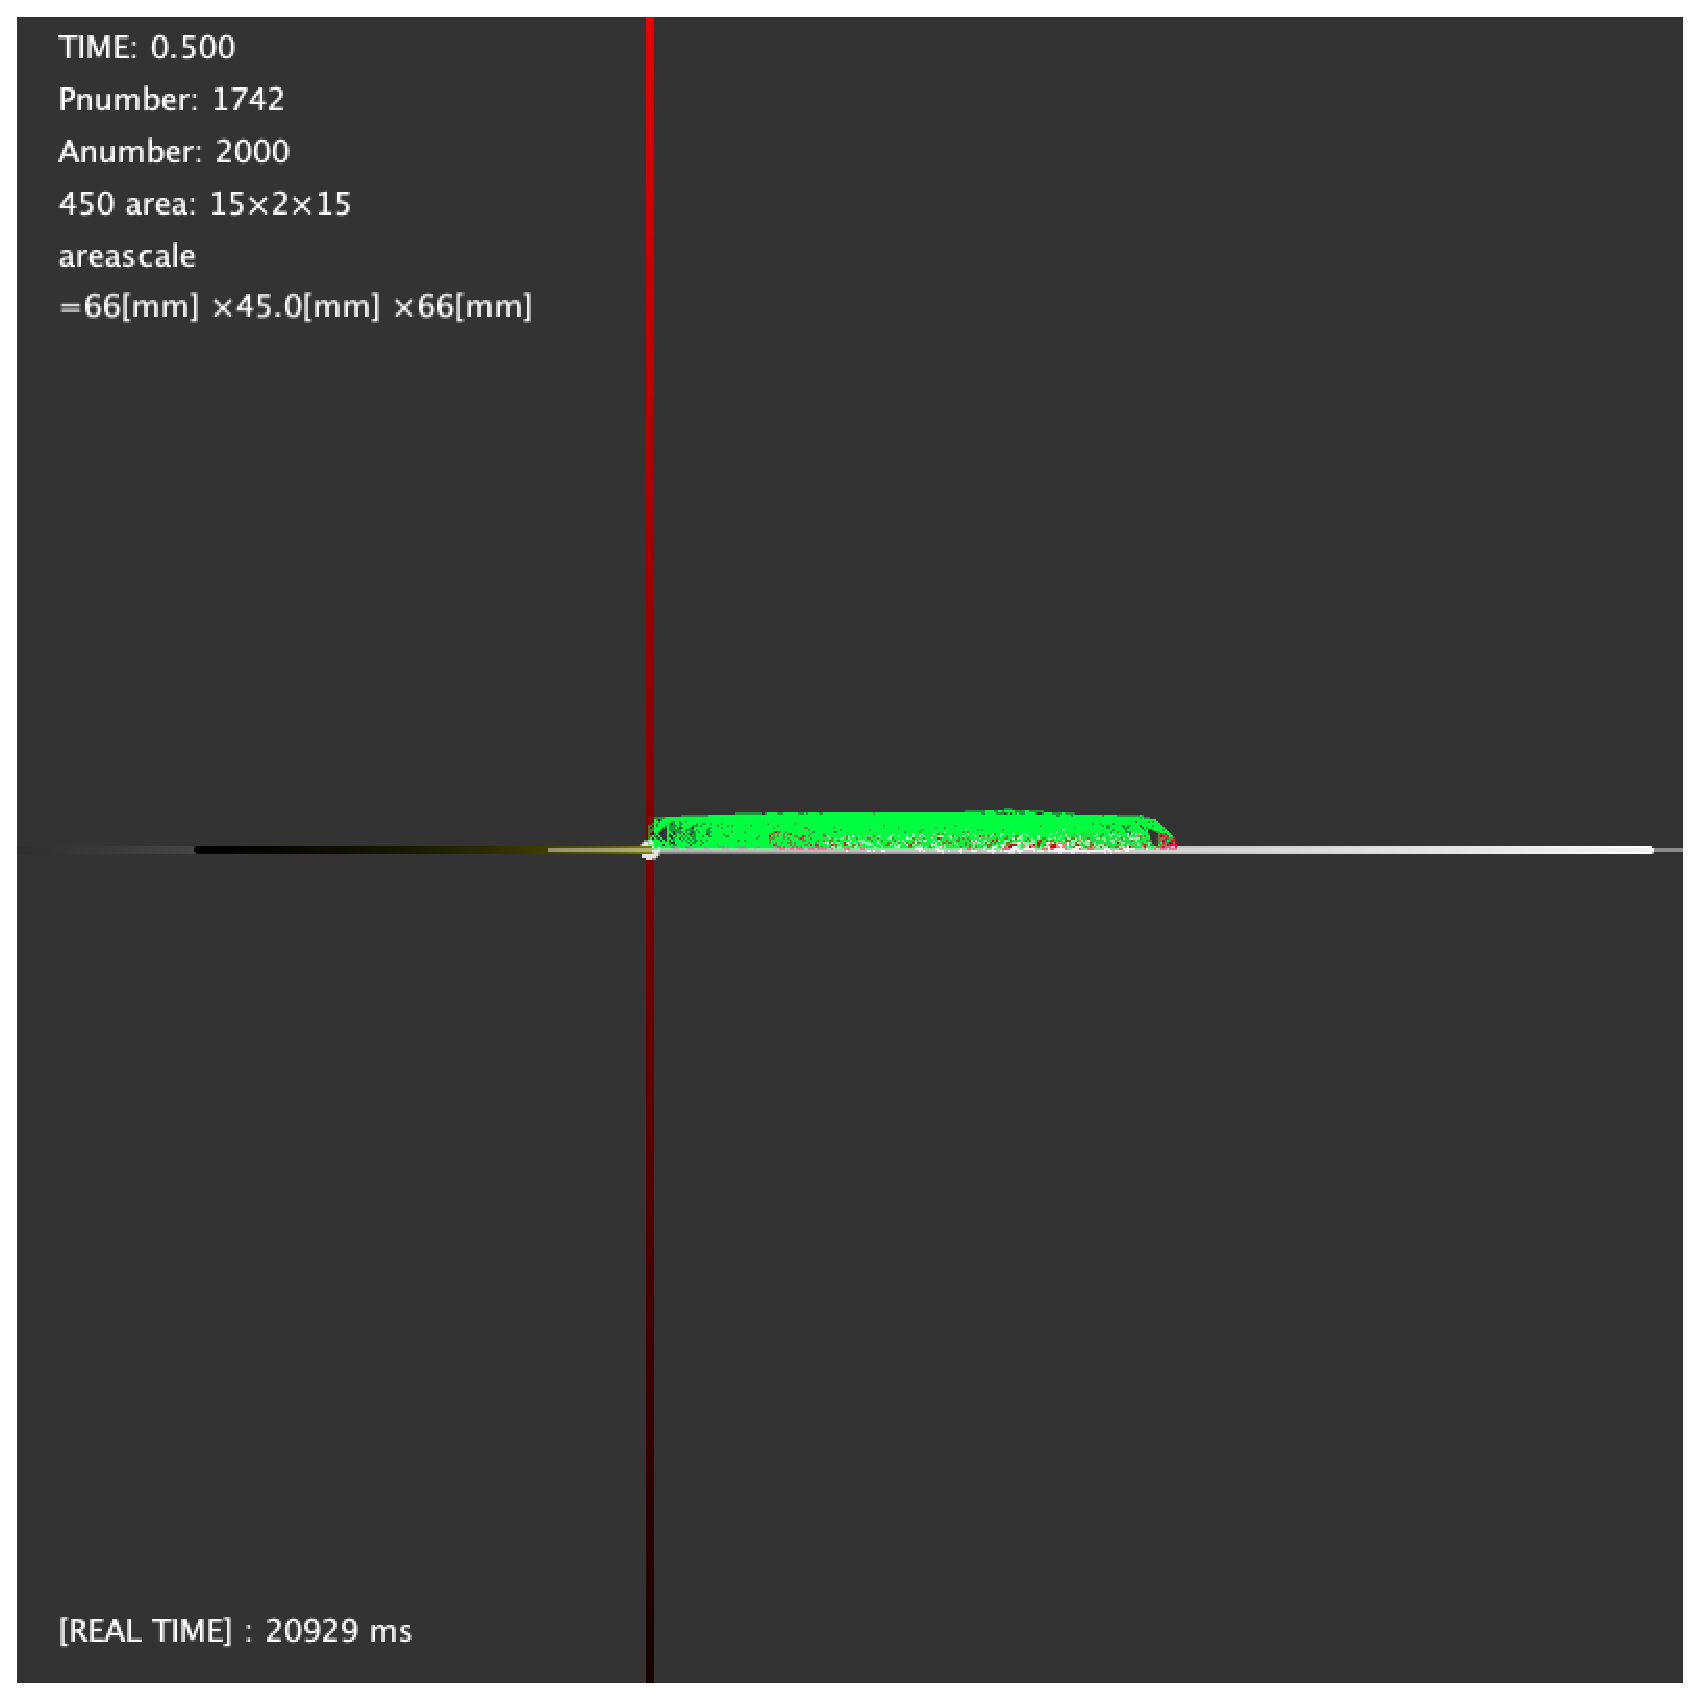
\includegraphics[width=5cm]{side05_2arf.eps}
  \end{tabular}
 }%
 \subfloat[t=2.0]{%
  \begin{tabular}{c}
   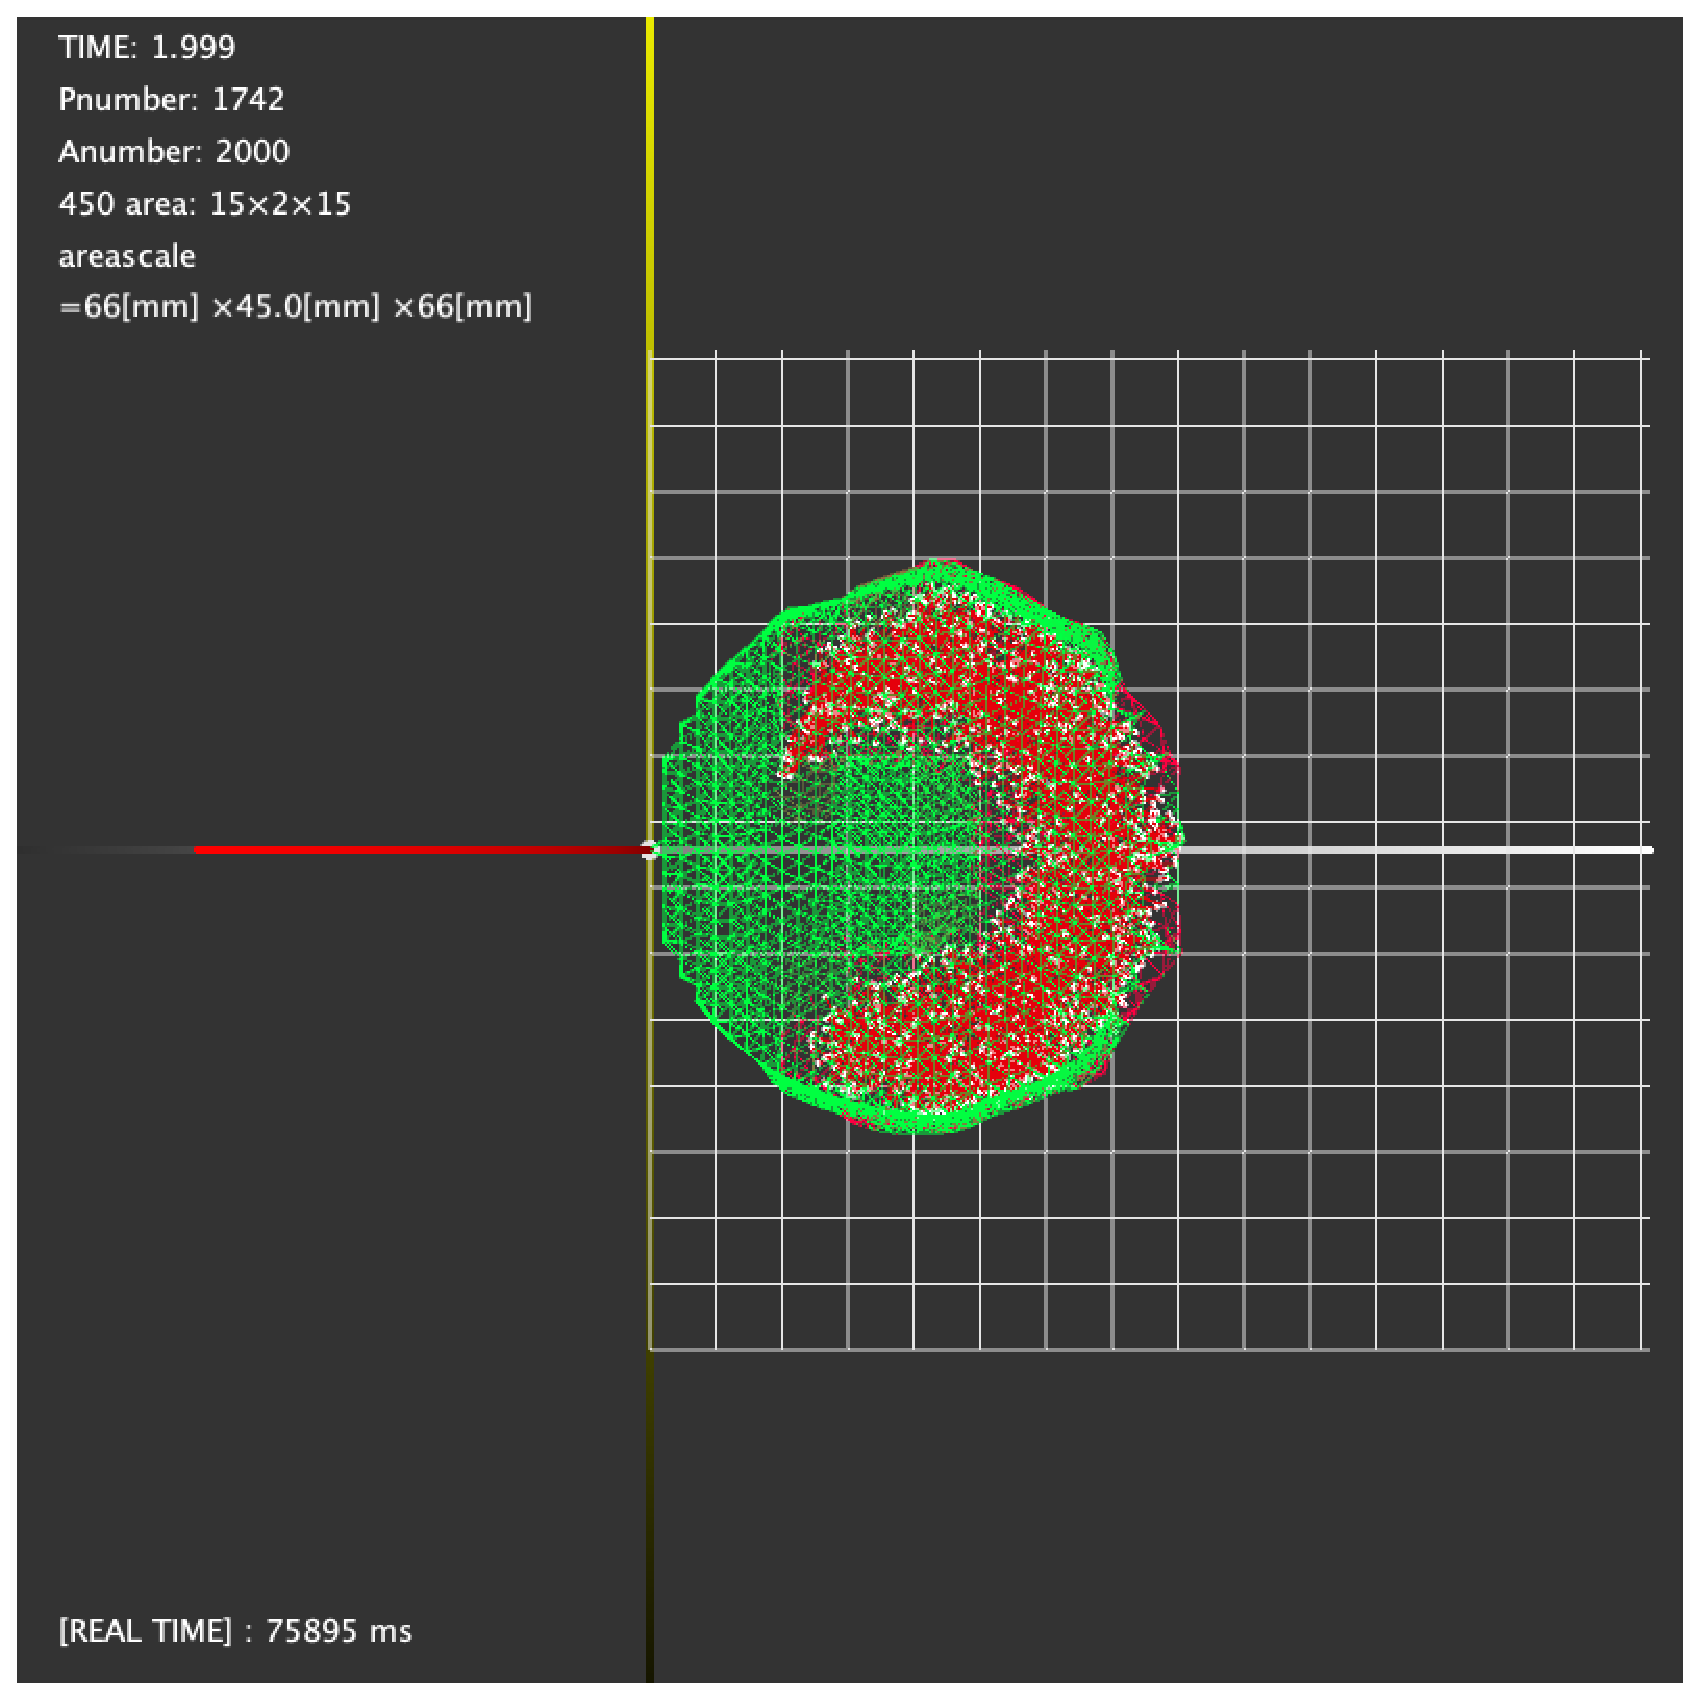
\includegraphics[width=5cm]{top20_2arf.eps} \\
   \includegraphics[width=5cm]{side20_2arf.eps}
  \end{tabular}
 }%
 \subfloat[t=4.0]{%
  \begin{tabular}{c}
   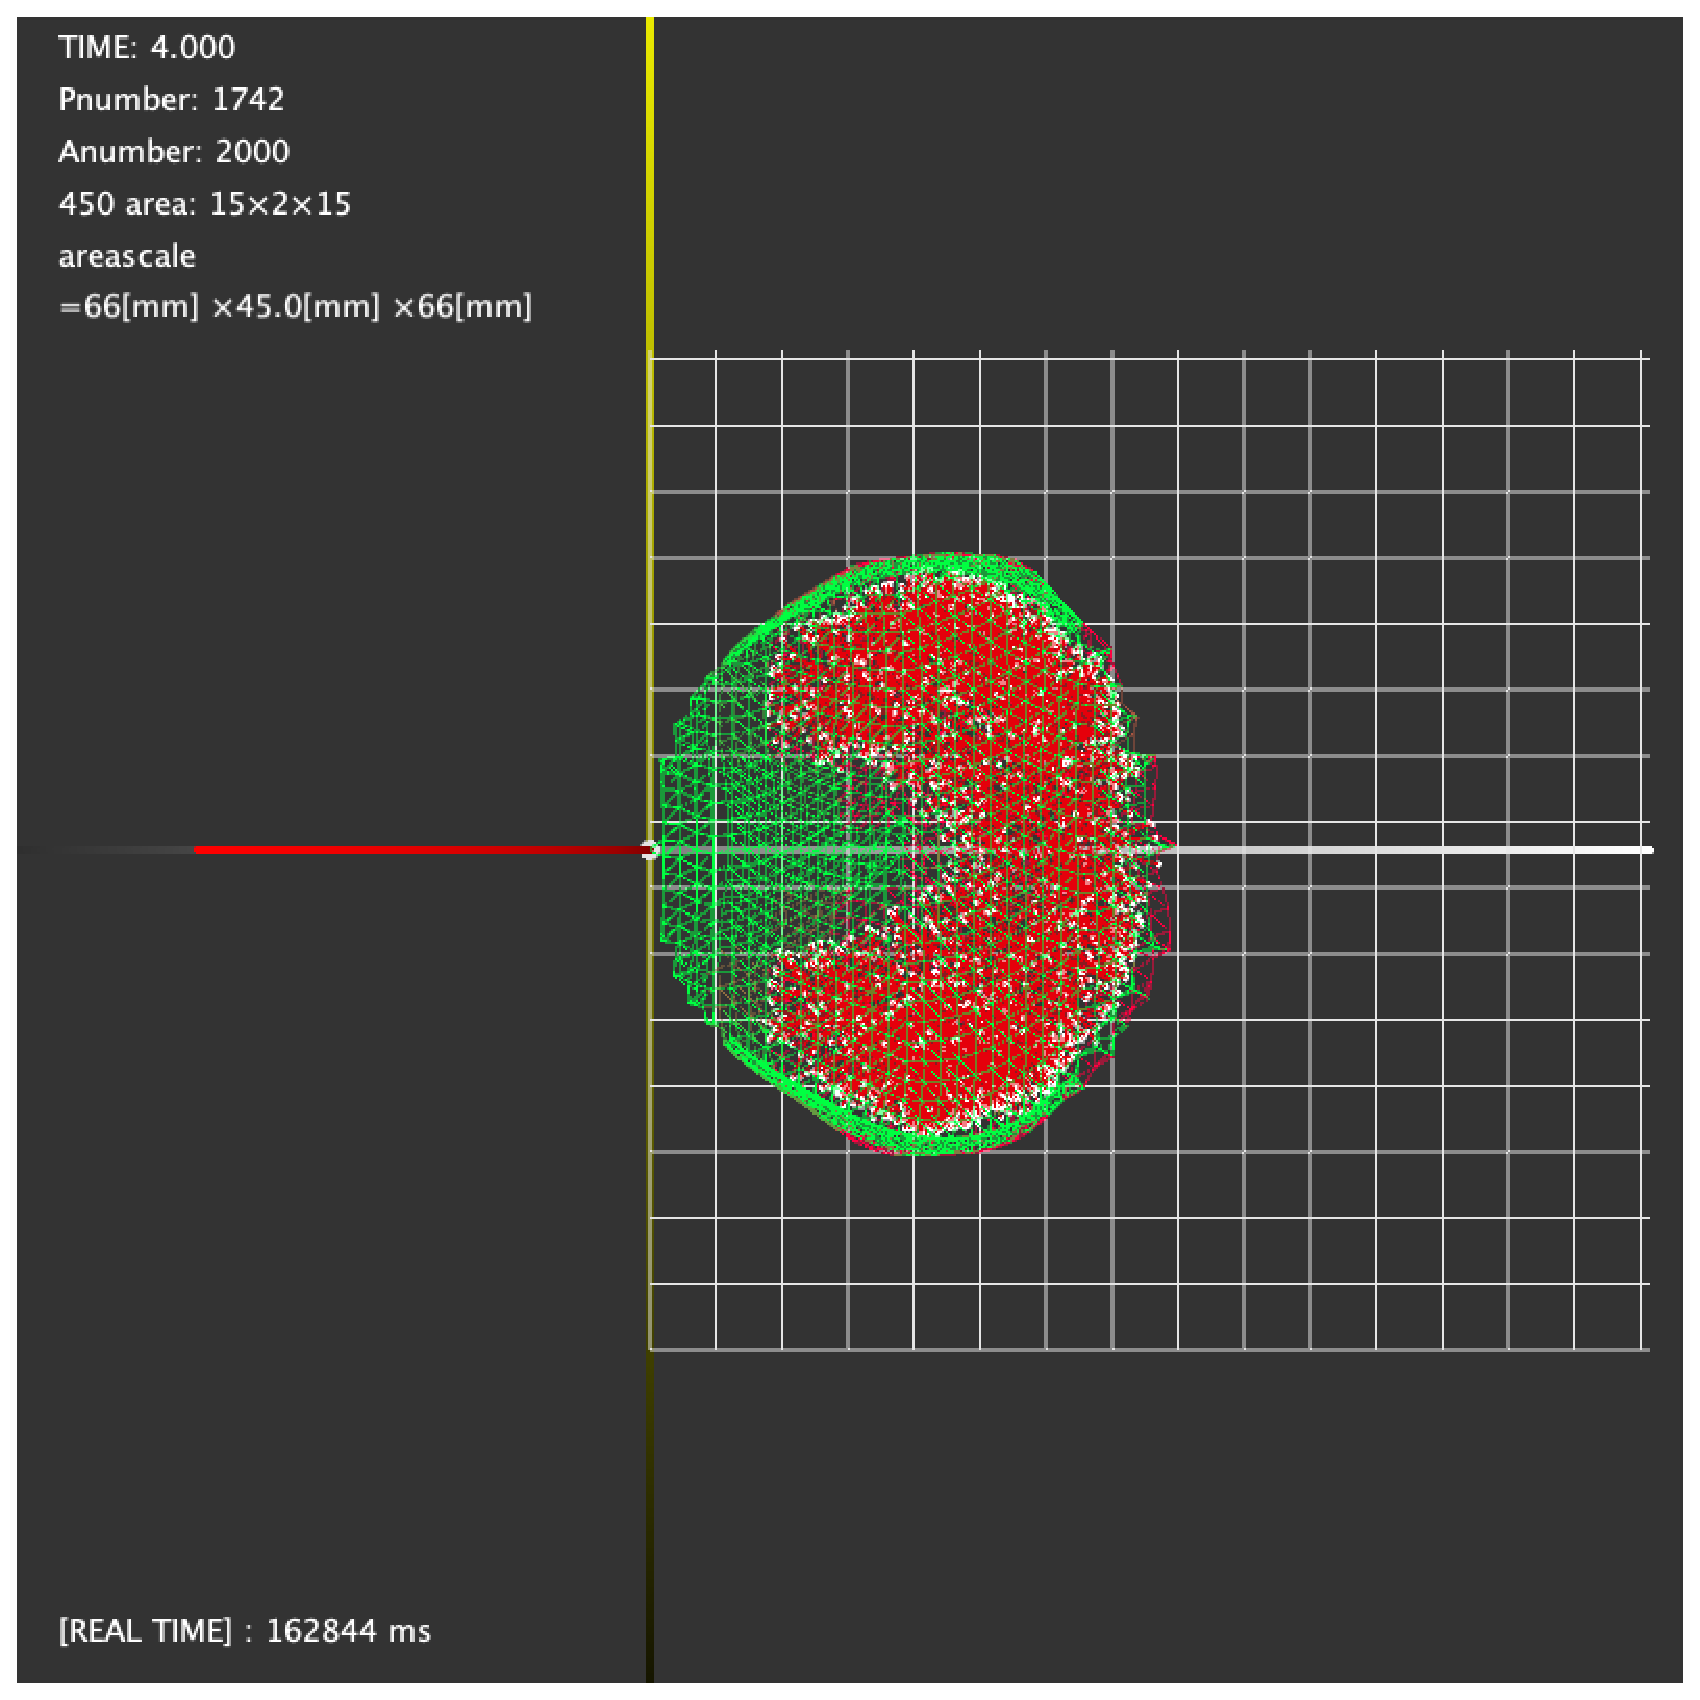
\includegraphics[width=5cm]{top40_2arf.eps} \\
   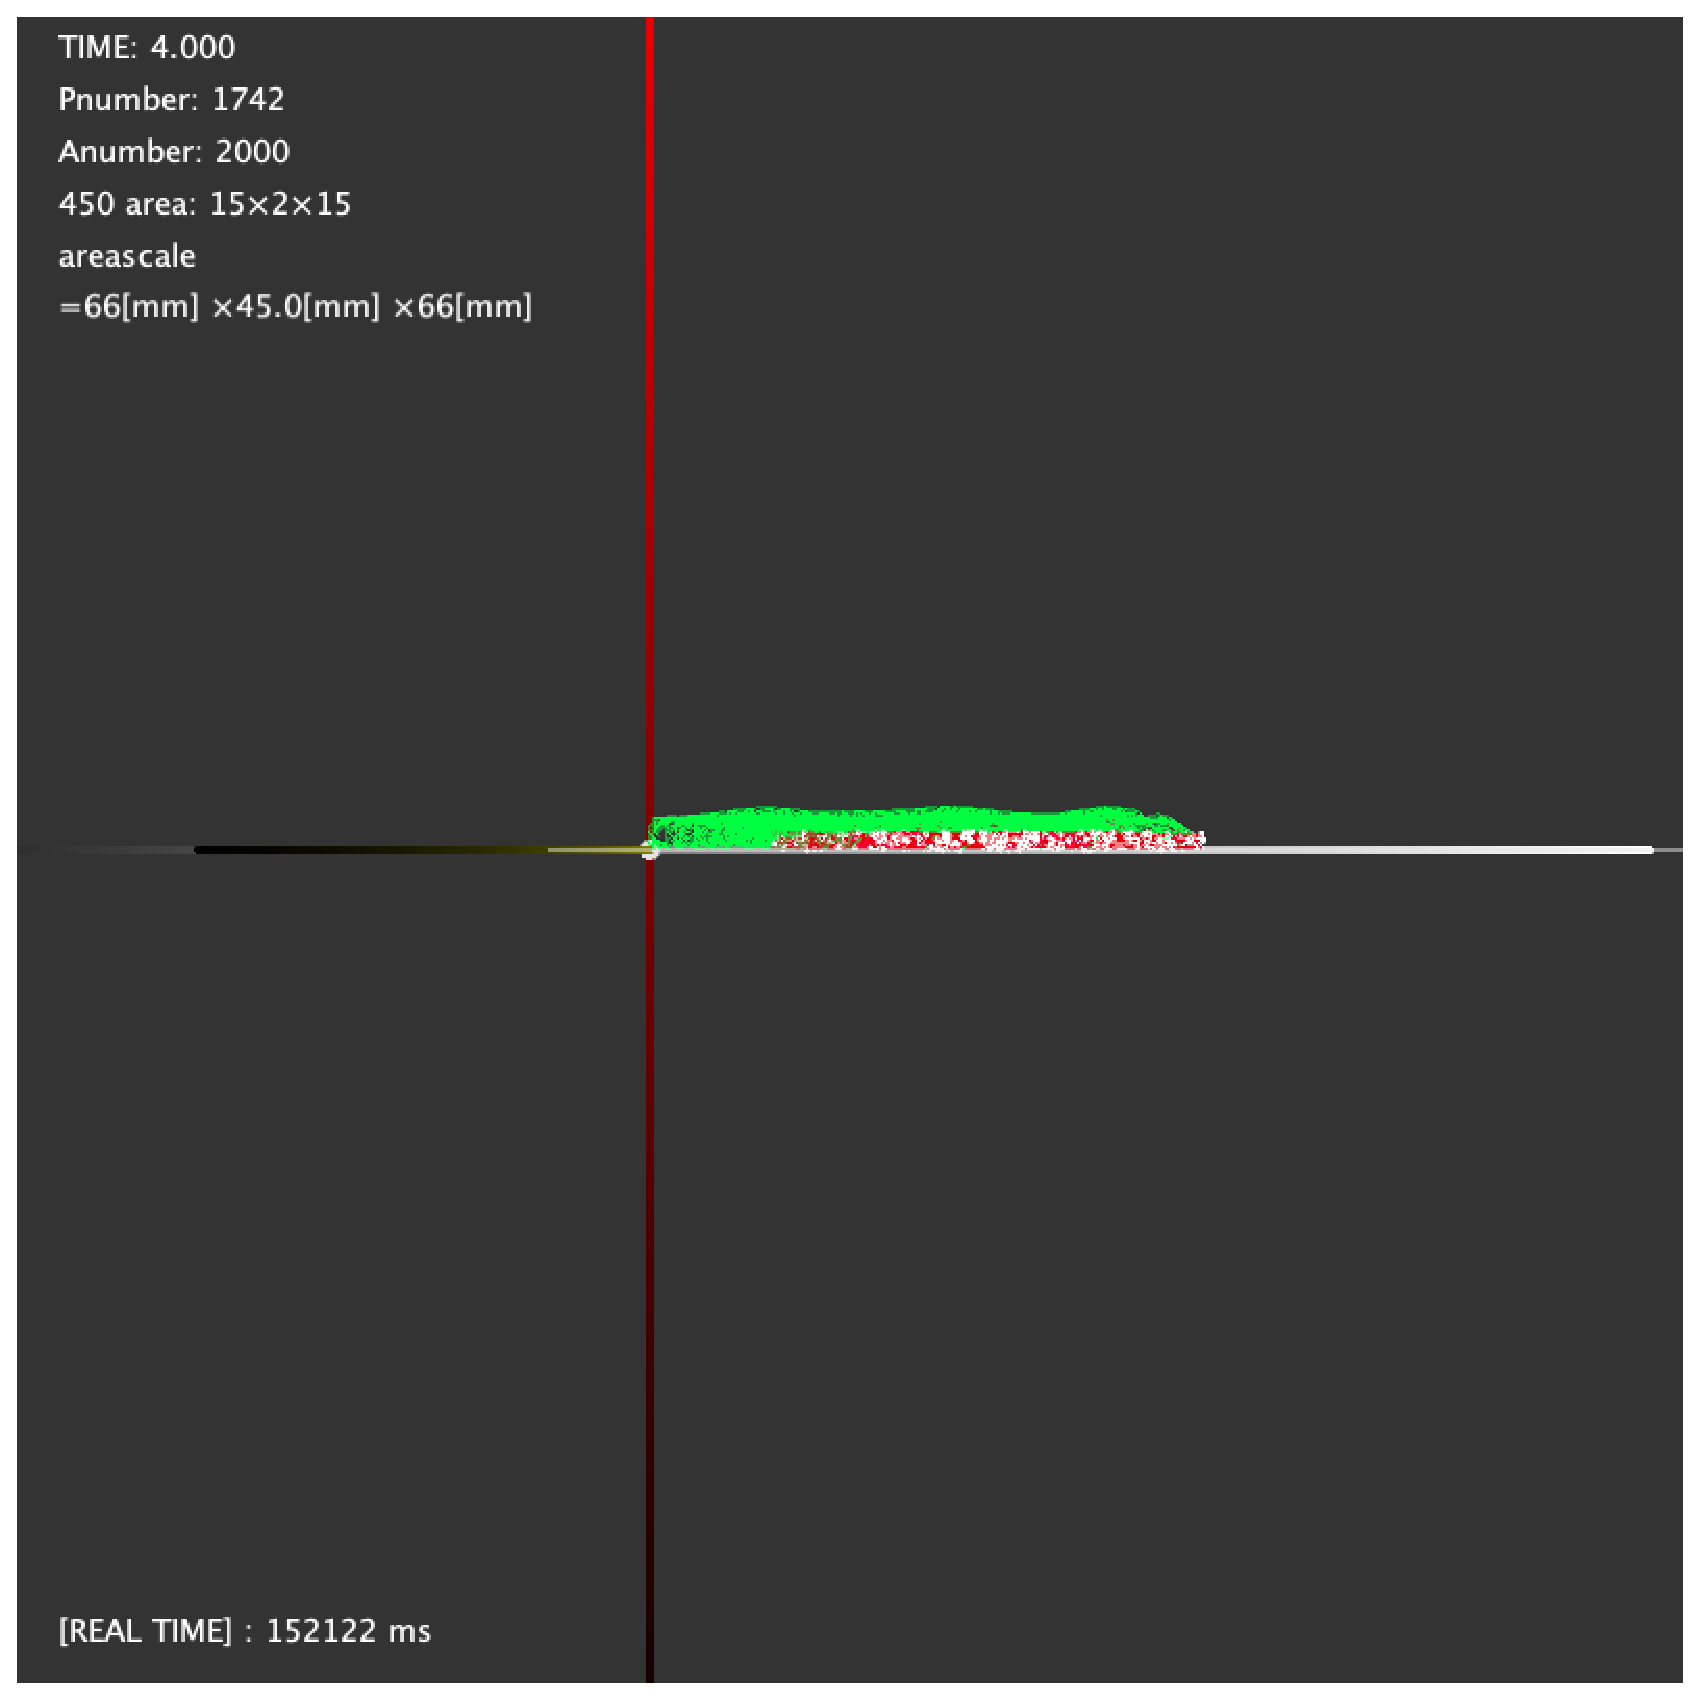
\includegraphics[width=5cm]{side40_2arf.eps}
  \end{tabular}
 }%
 \caption{Simulation results using ARF with patterns with two reference points.}
 \label{fig:res3}
\end{figure}

Fig. \ref{fig:res3} shows the simulation results when using ARF reference points $\bm{E}_1$ and $\bm{E}_2$ instead of $\bm{E}_0$.

\subsection{Importance of Relocation Condition}

\begin{figure}[h]
 \subfloat[t=0.5.]{%
  \begin{tabular}{c}
   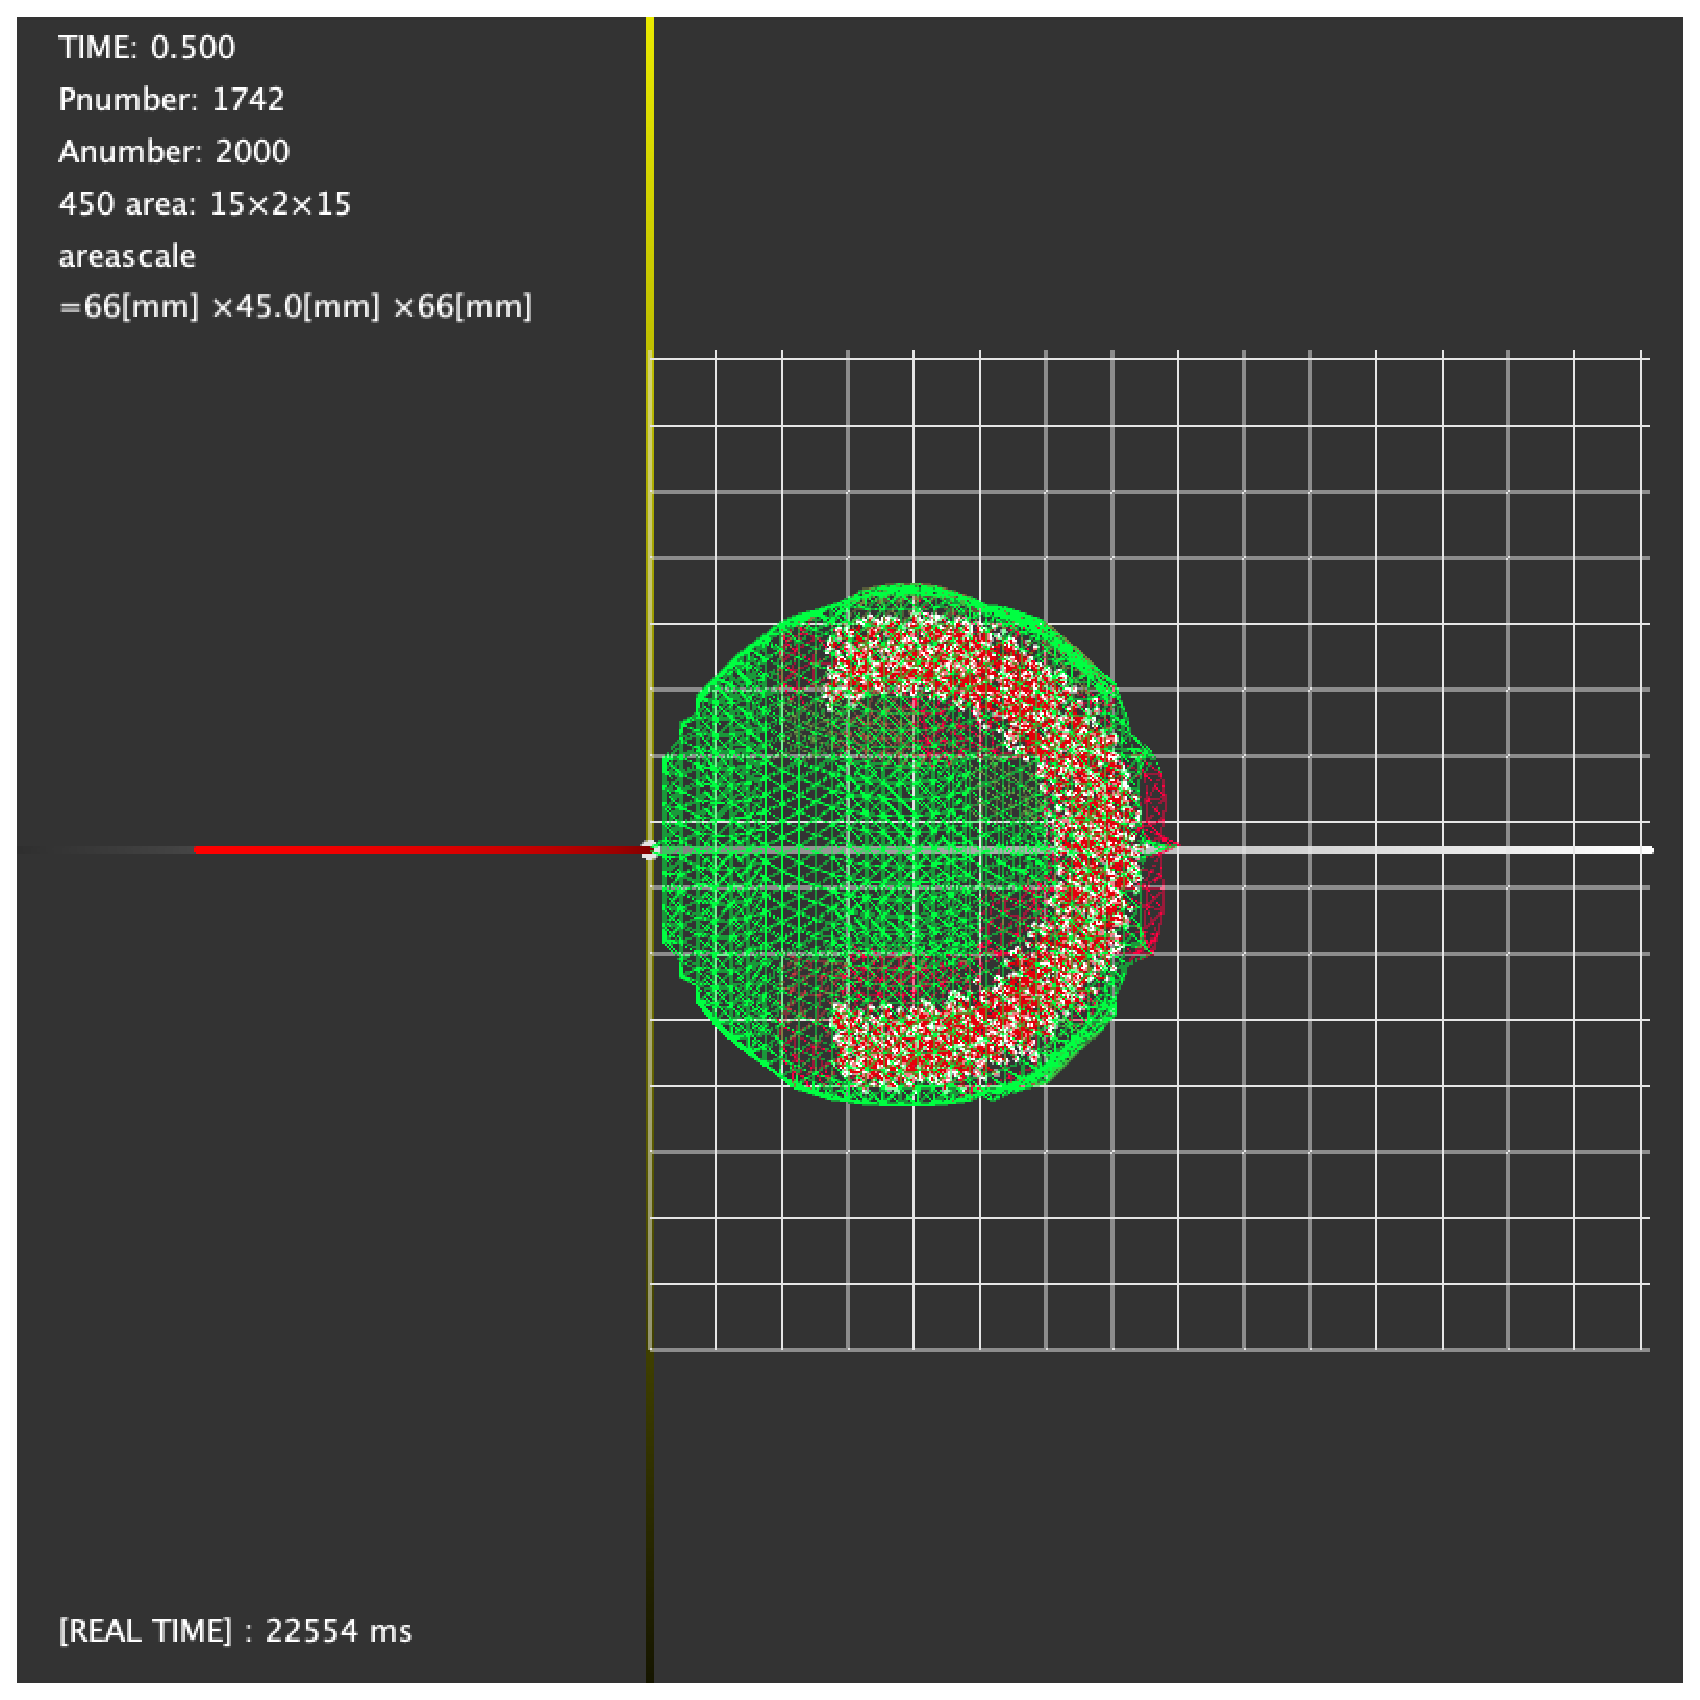
\includegraphics[width=5cm]{top05_15rc.eps} \\
   \includegraphics[width=5cm]{side05_15rc.eps}
  \end{tabular}
 }%
 \subfloat[t=2.0]{%
  \begin{tabular}{c}
   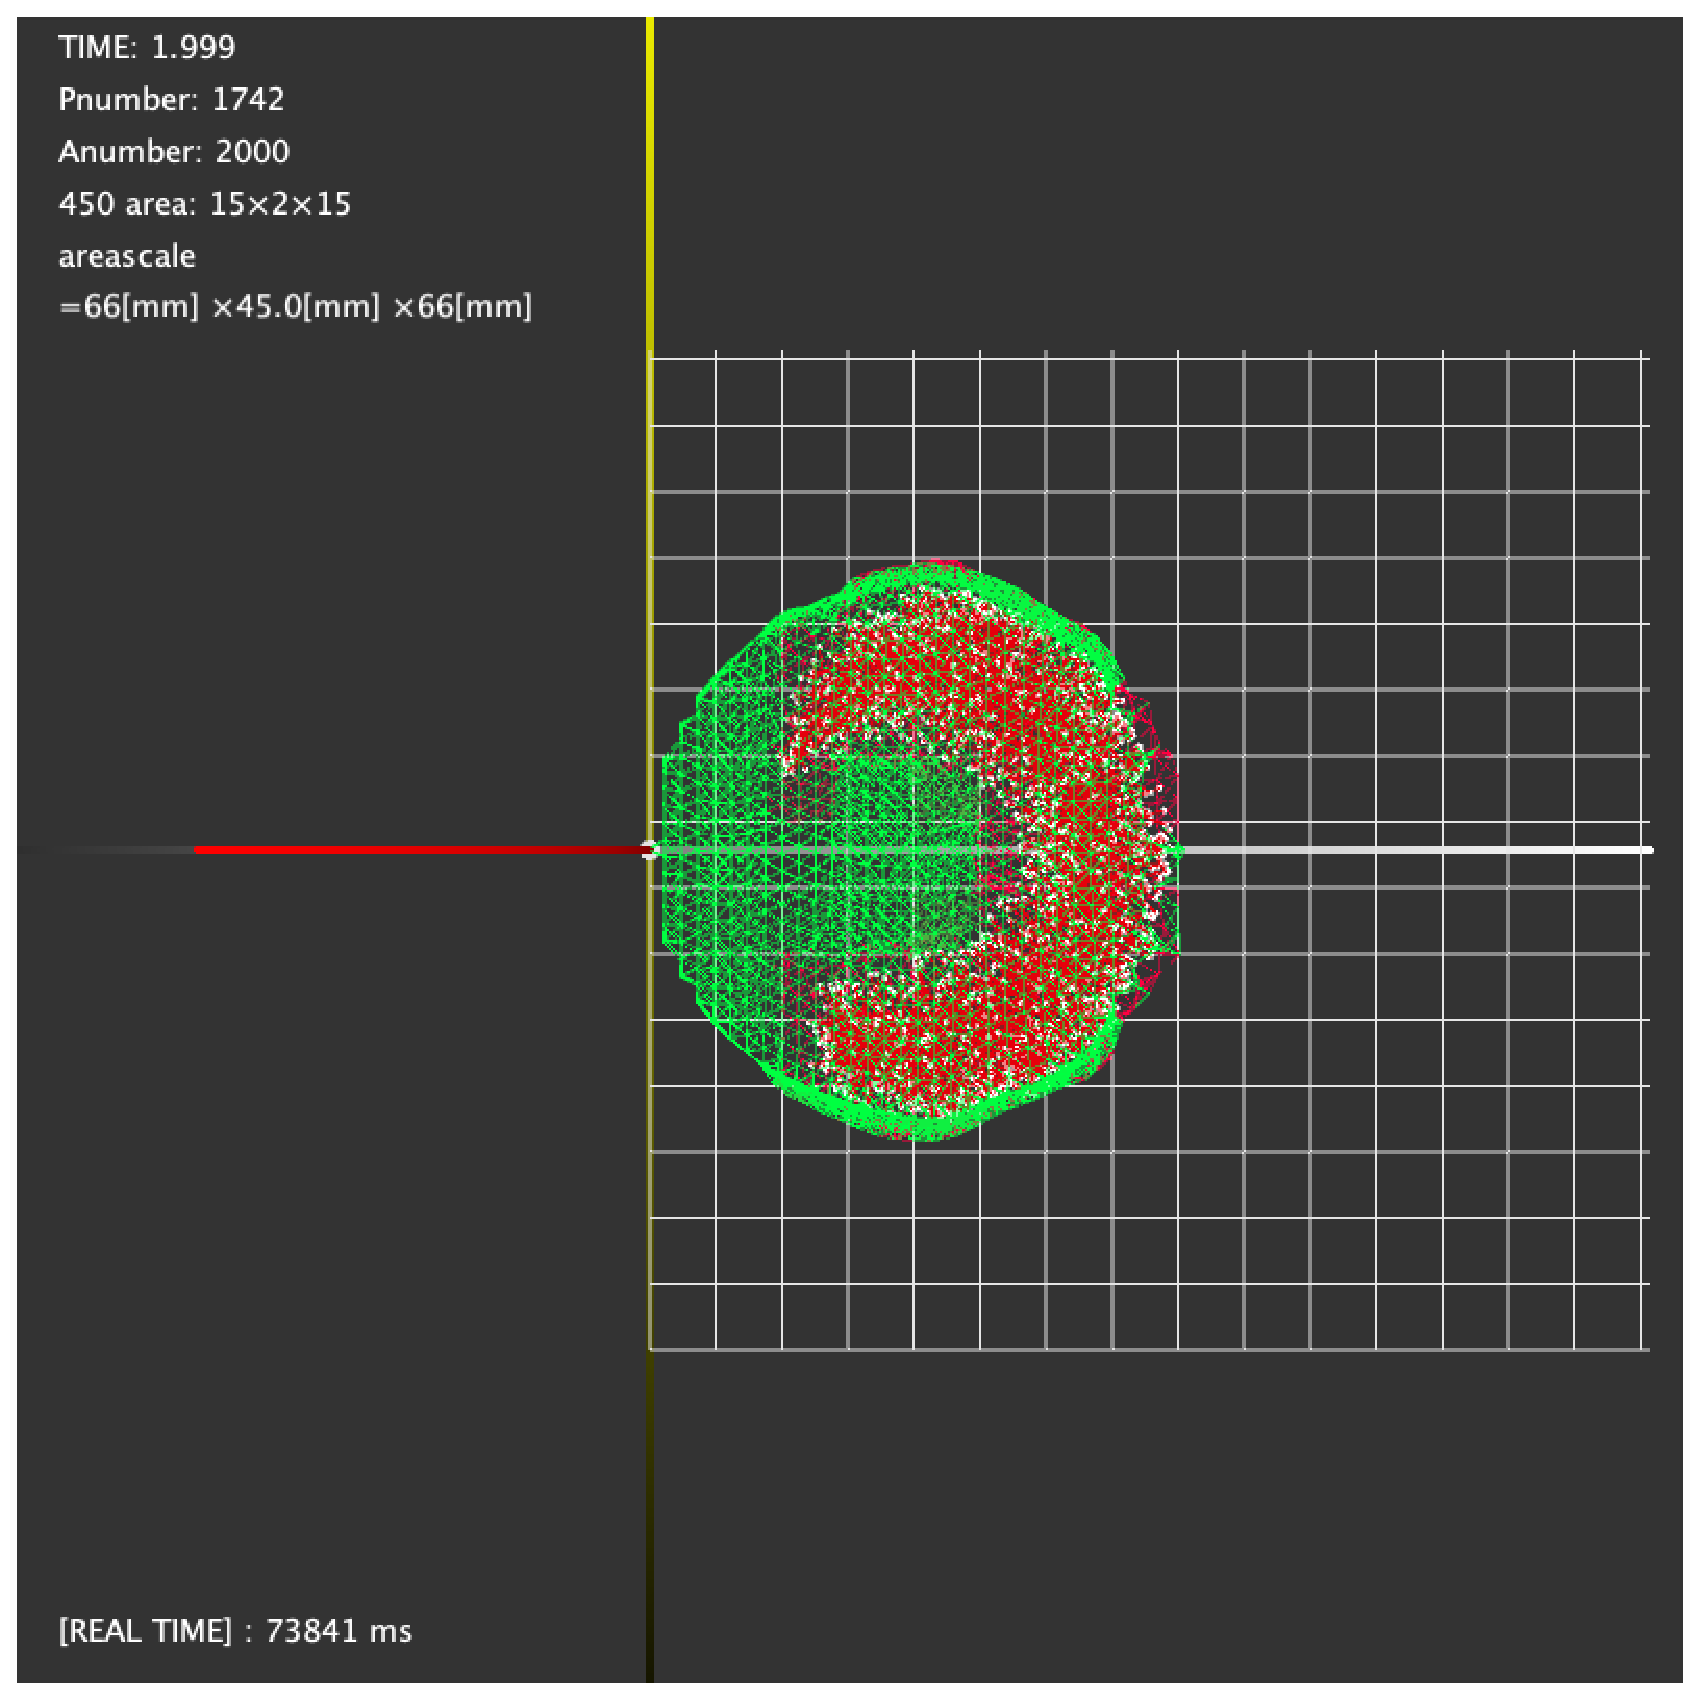
\includegraphics[width=5cm]{top20_15rc.eps} \\
   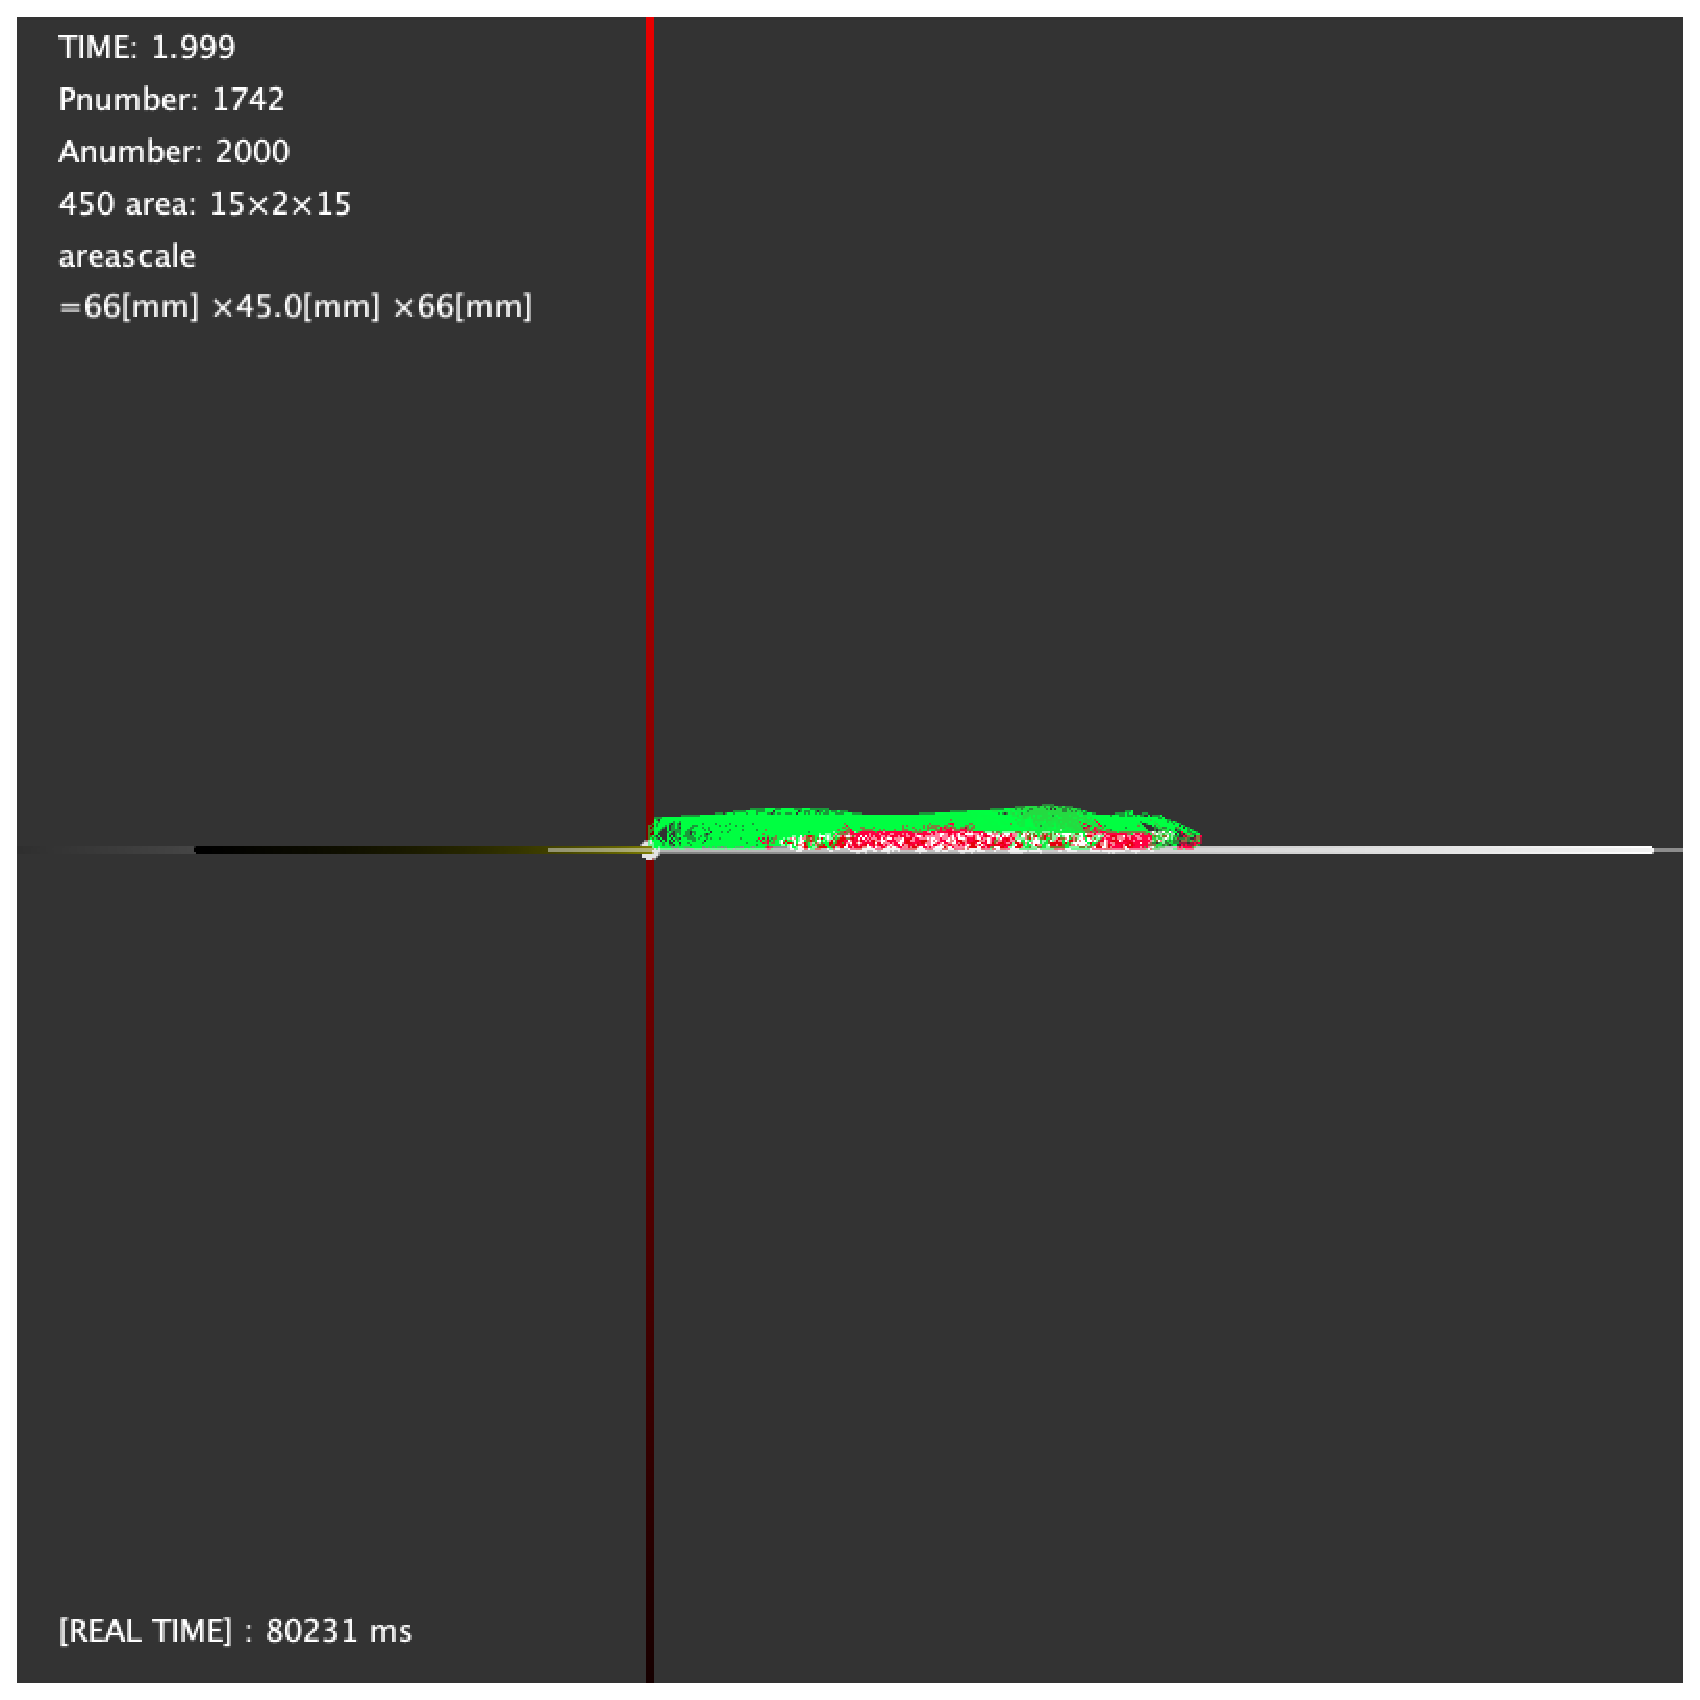
\includegraphics[width=5cm]{side20_15rc.eps}
  \end{tabular}
 }%
 \subfloat[t=4.0]{%
  \begin{tabular}{c}
   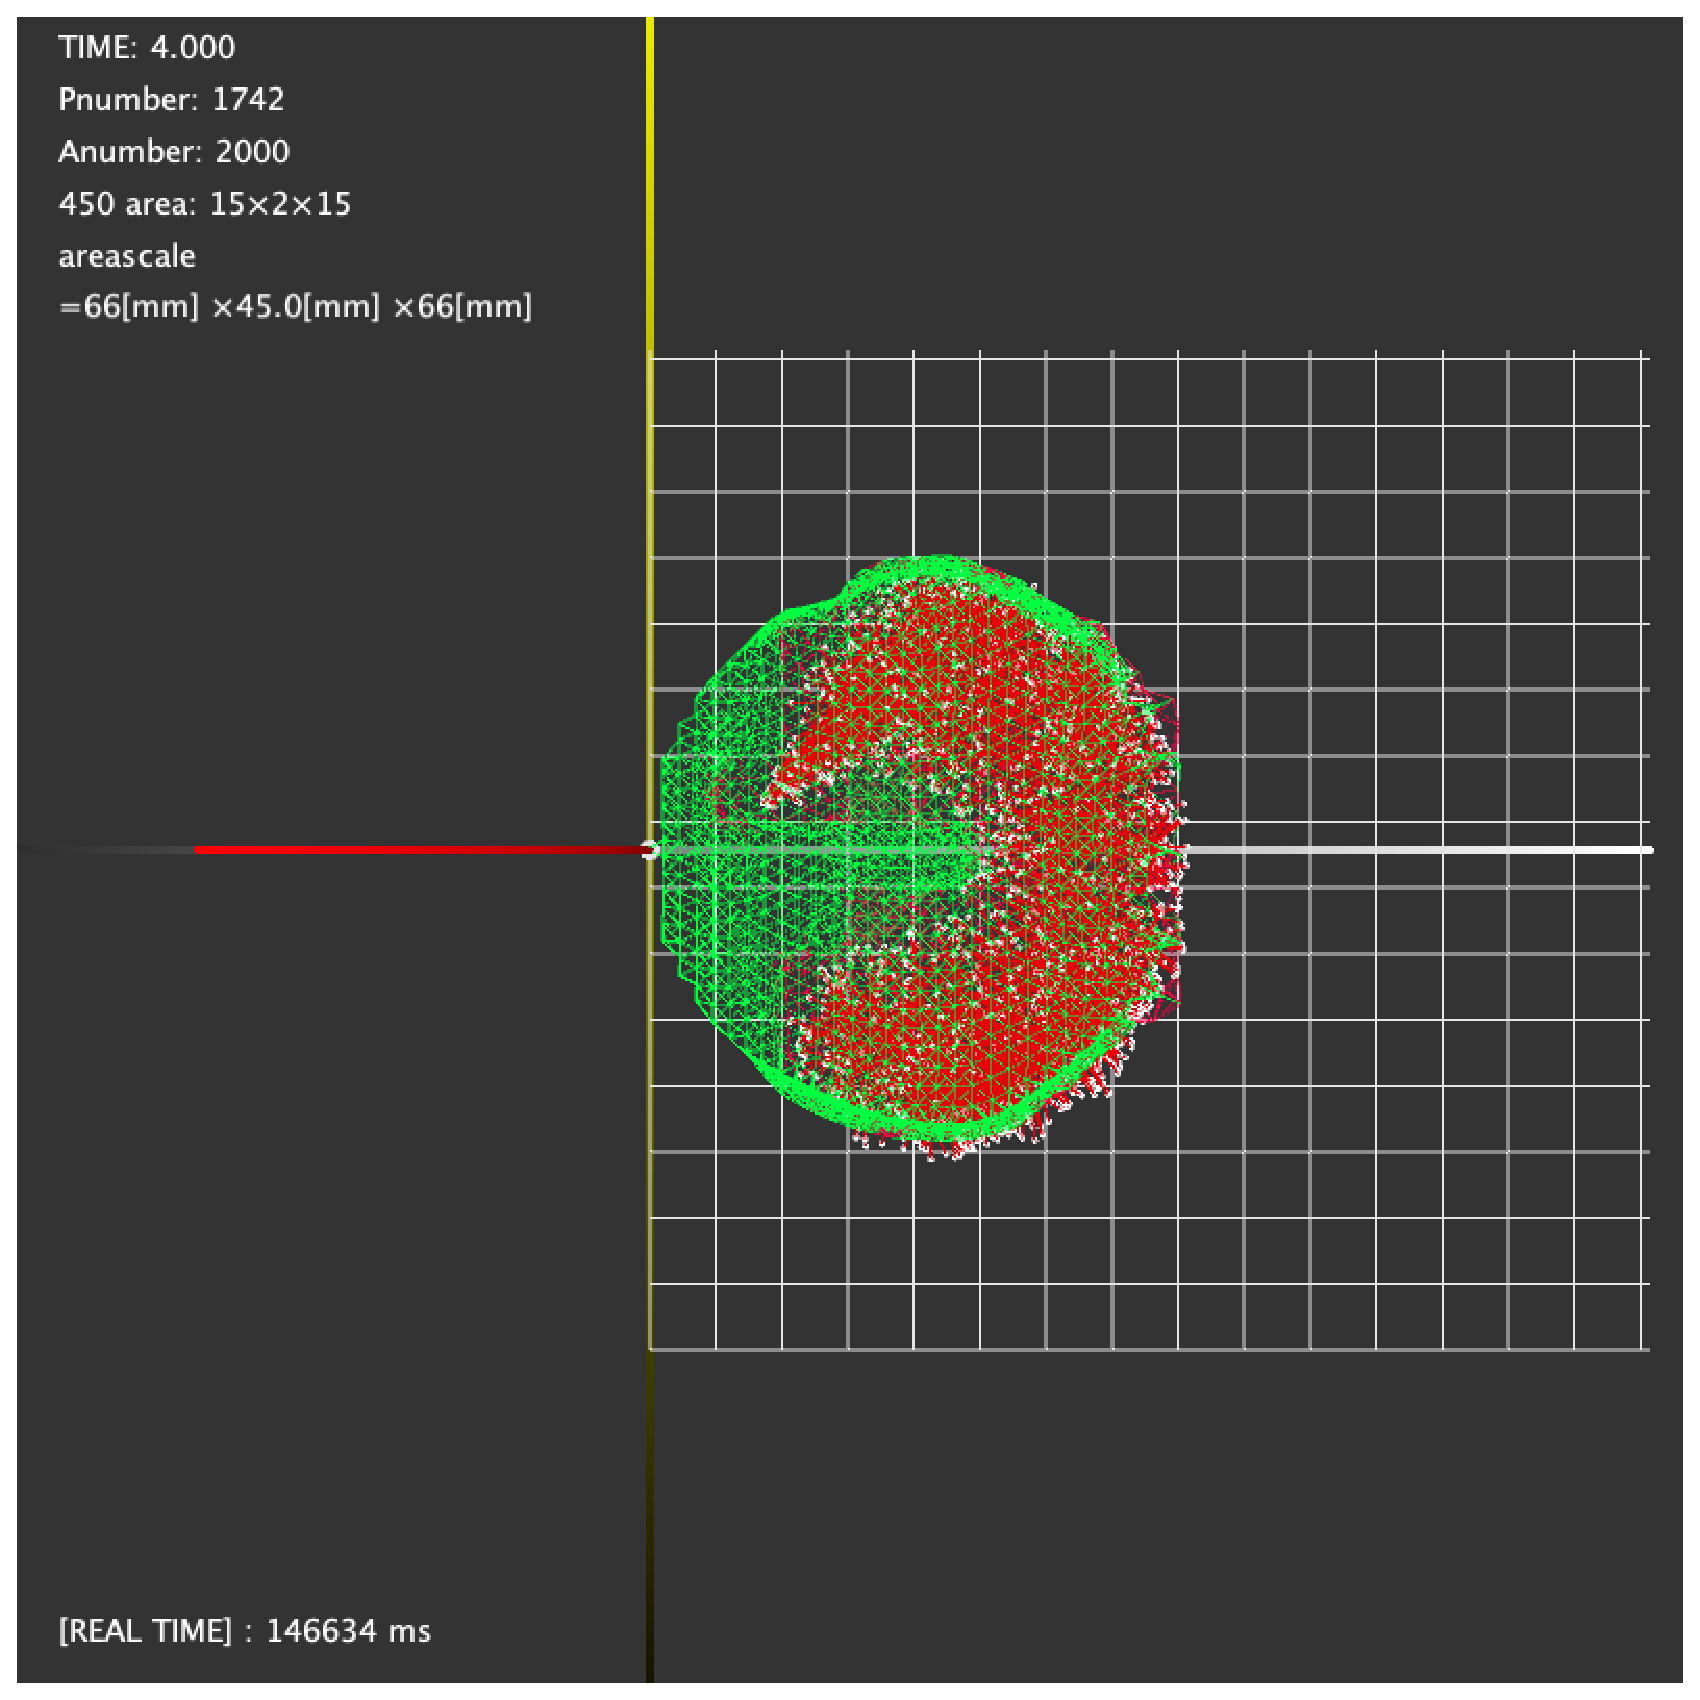
\includegraphics[width=5cm]{top40_15rc.eps} \\
   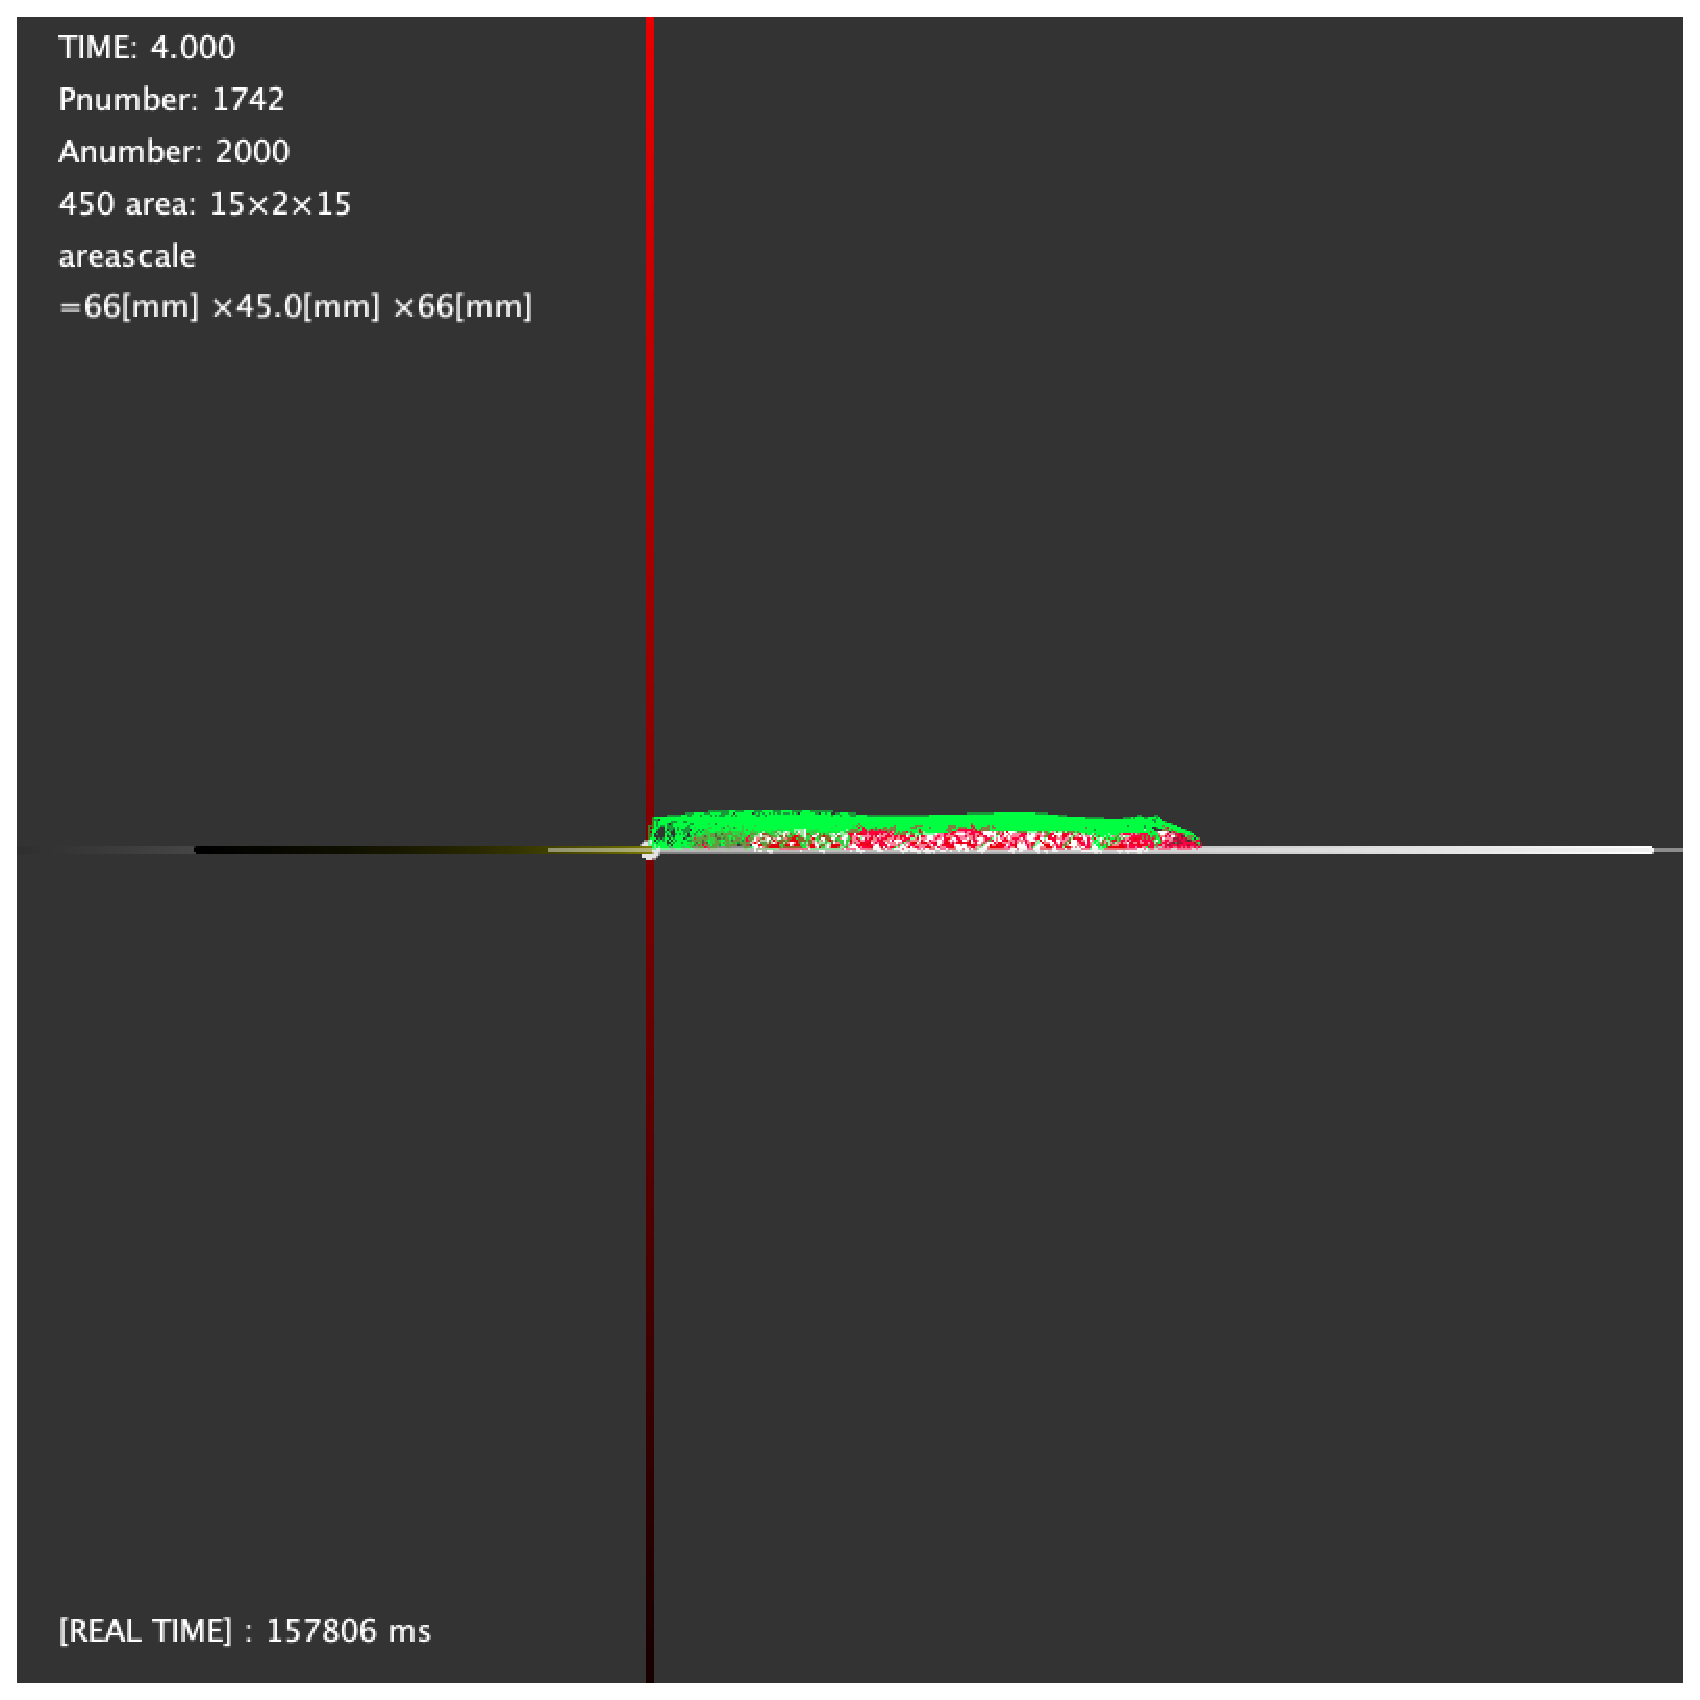
\includegraphics[width=5cm]{side40_15rc.eps}
  \end{tabular}
 }%
 \caption{Simulation results for relocation condition of actin concentration 1.5\%.}
 \label{fig:res4}
\end{figure}

\begin{figure}[h]
 \subfloat[t=0.5.]{%
  \begin{tabular}{c}
   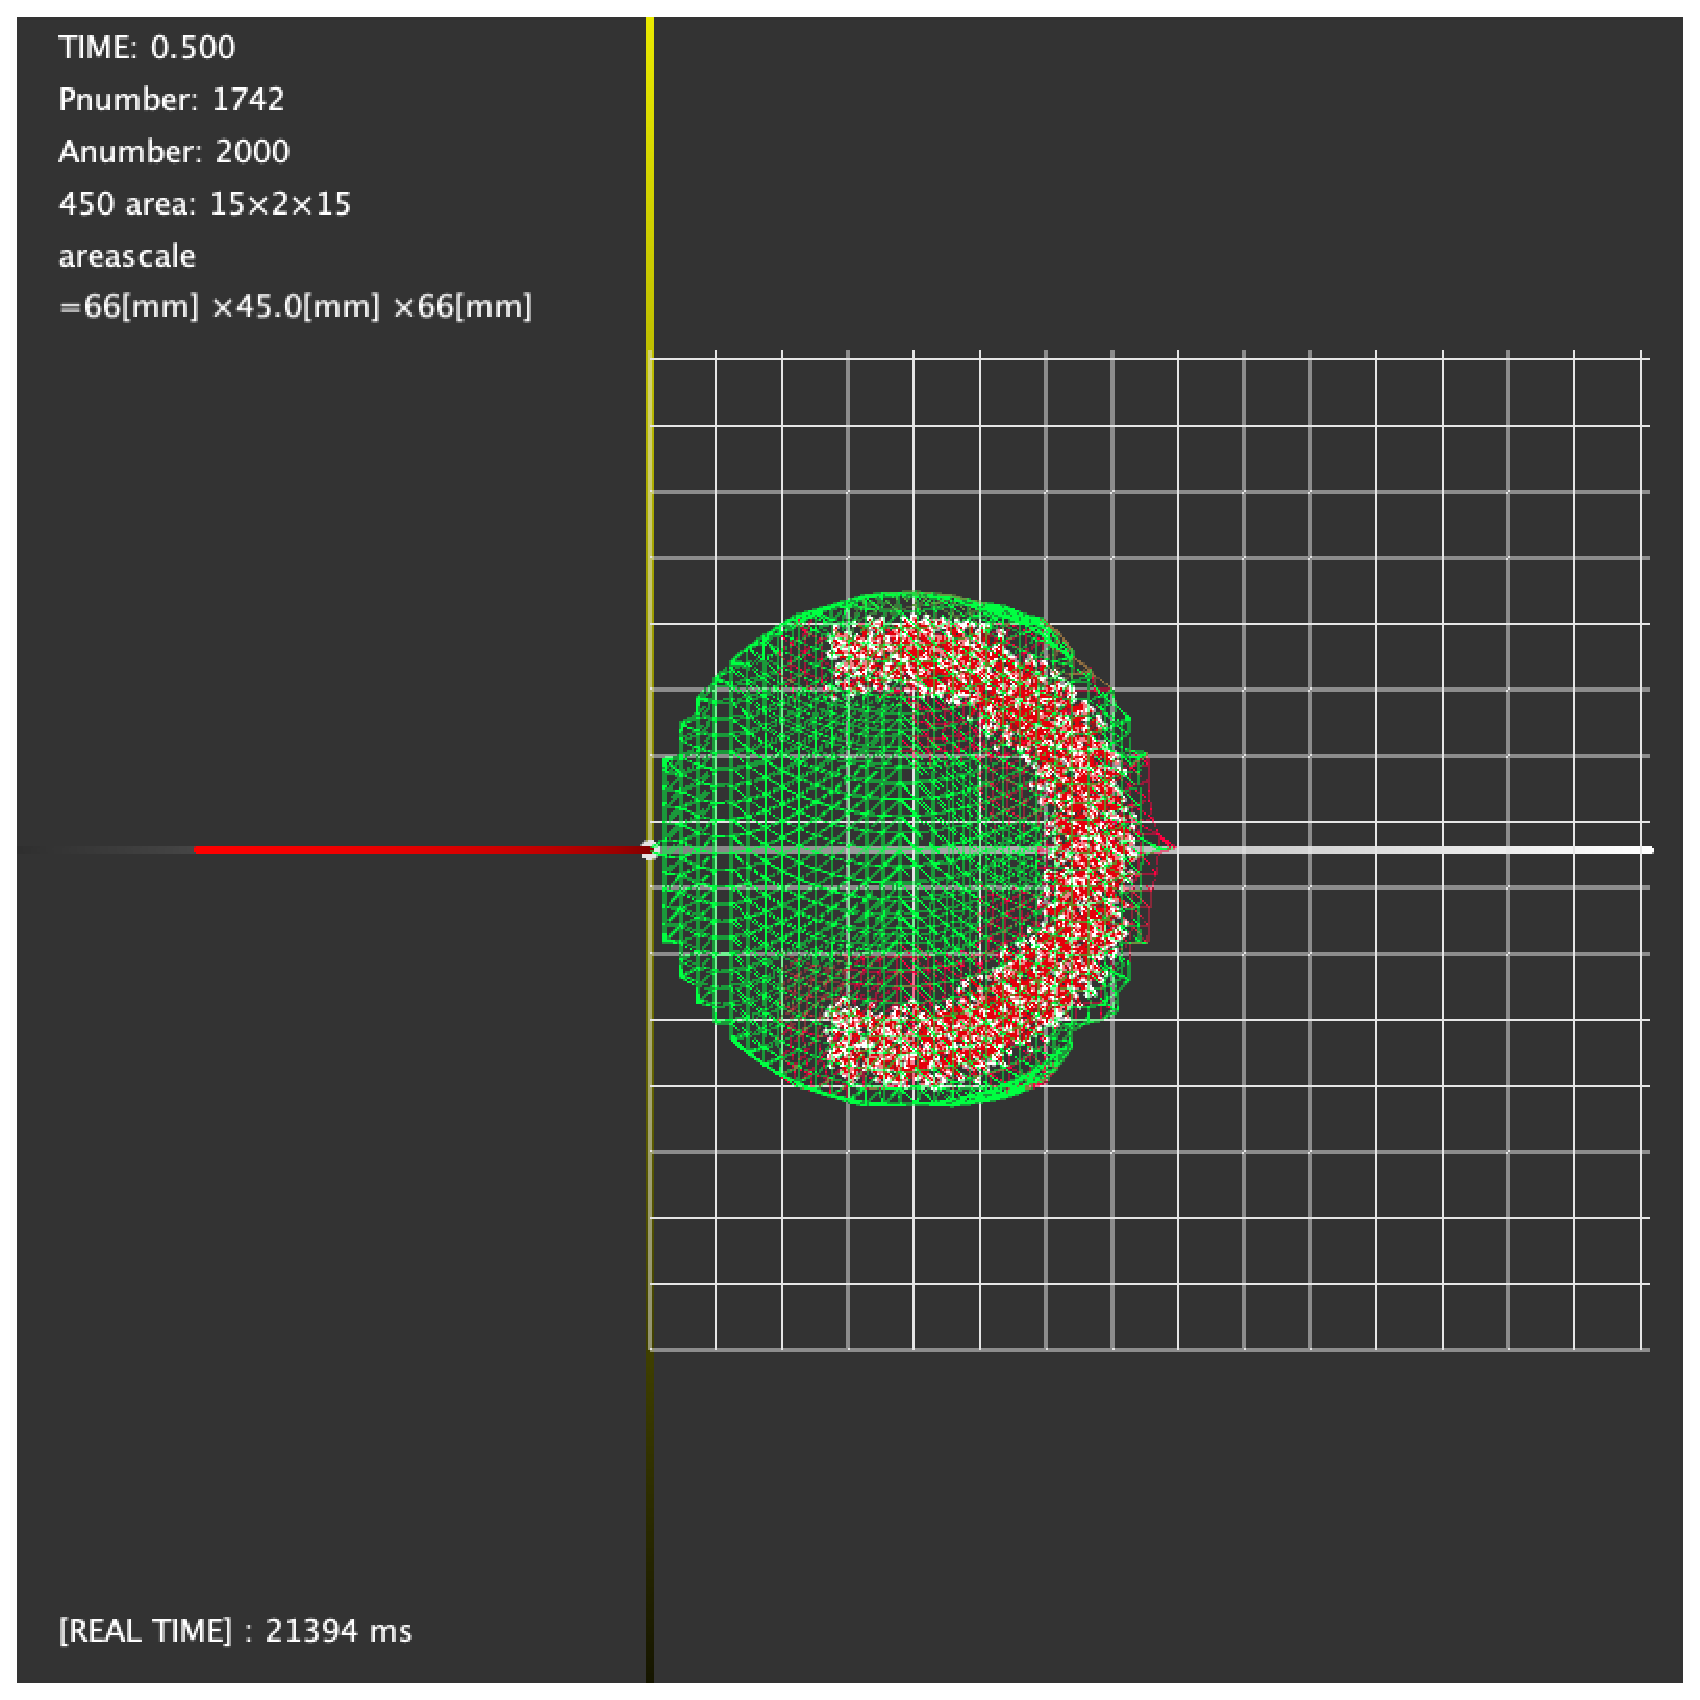
\includegraphics[width=5cm]{top05_25rc.eps} \\
   \includegraphics[width=5cm]{side05_25rc.eps}
  \end{tabular}
 }%
 \subfloat[t=2.0]{%
  \begin{tabular}{c}
   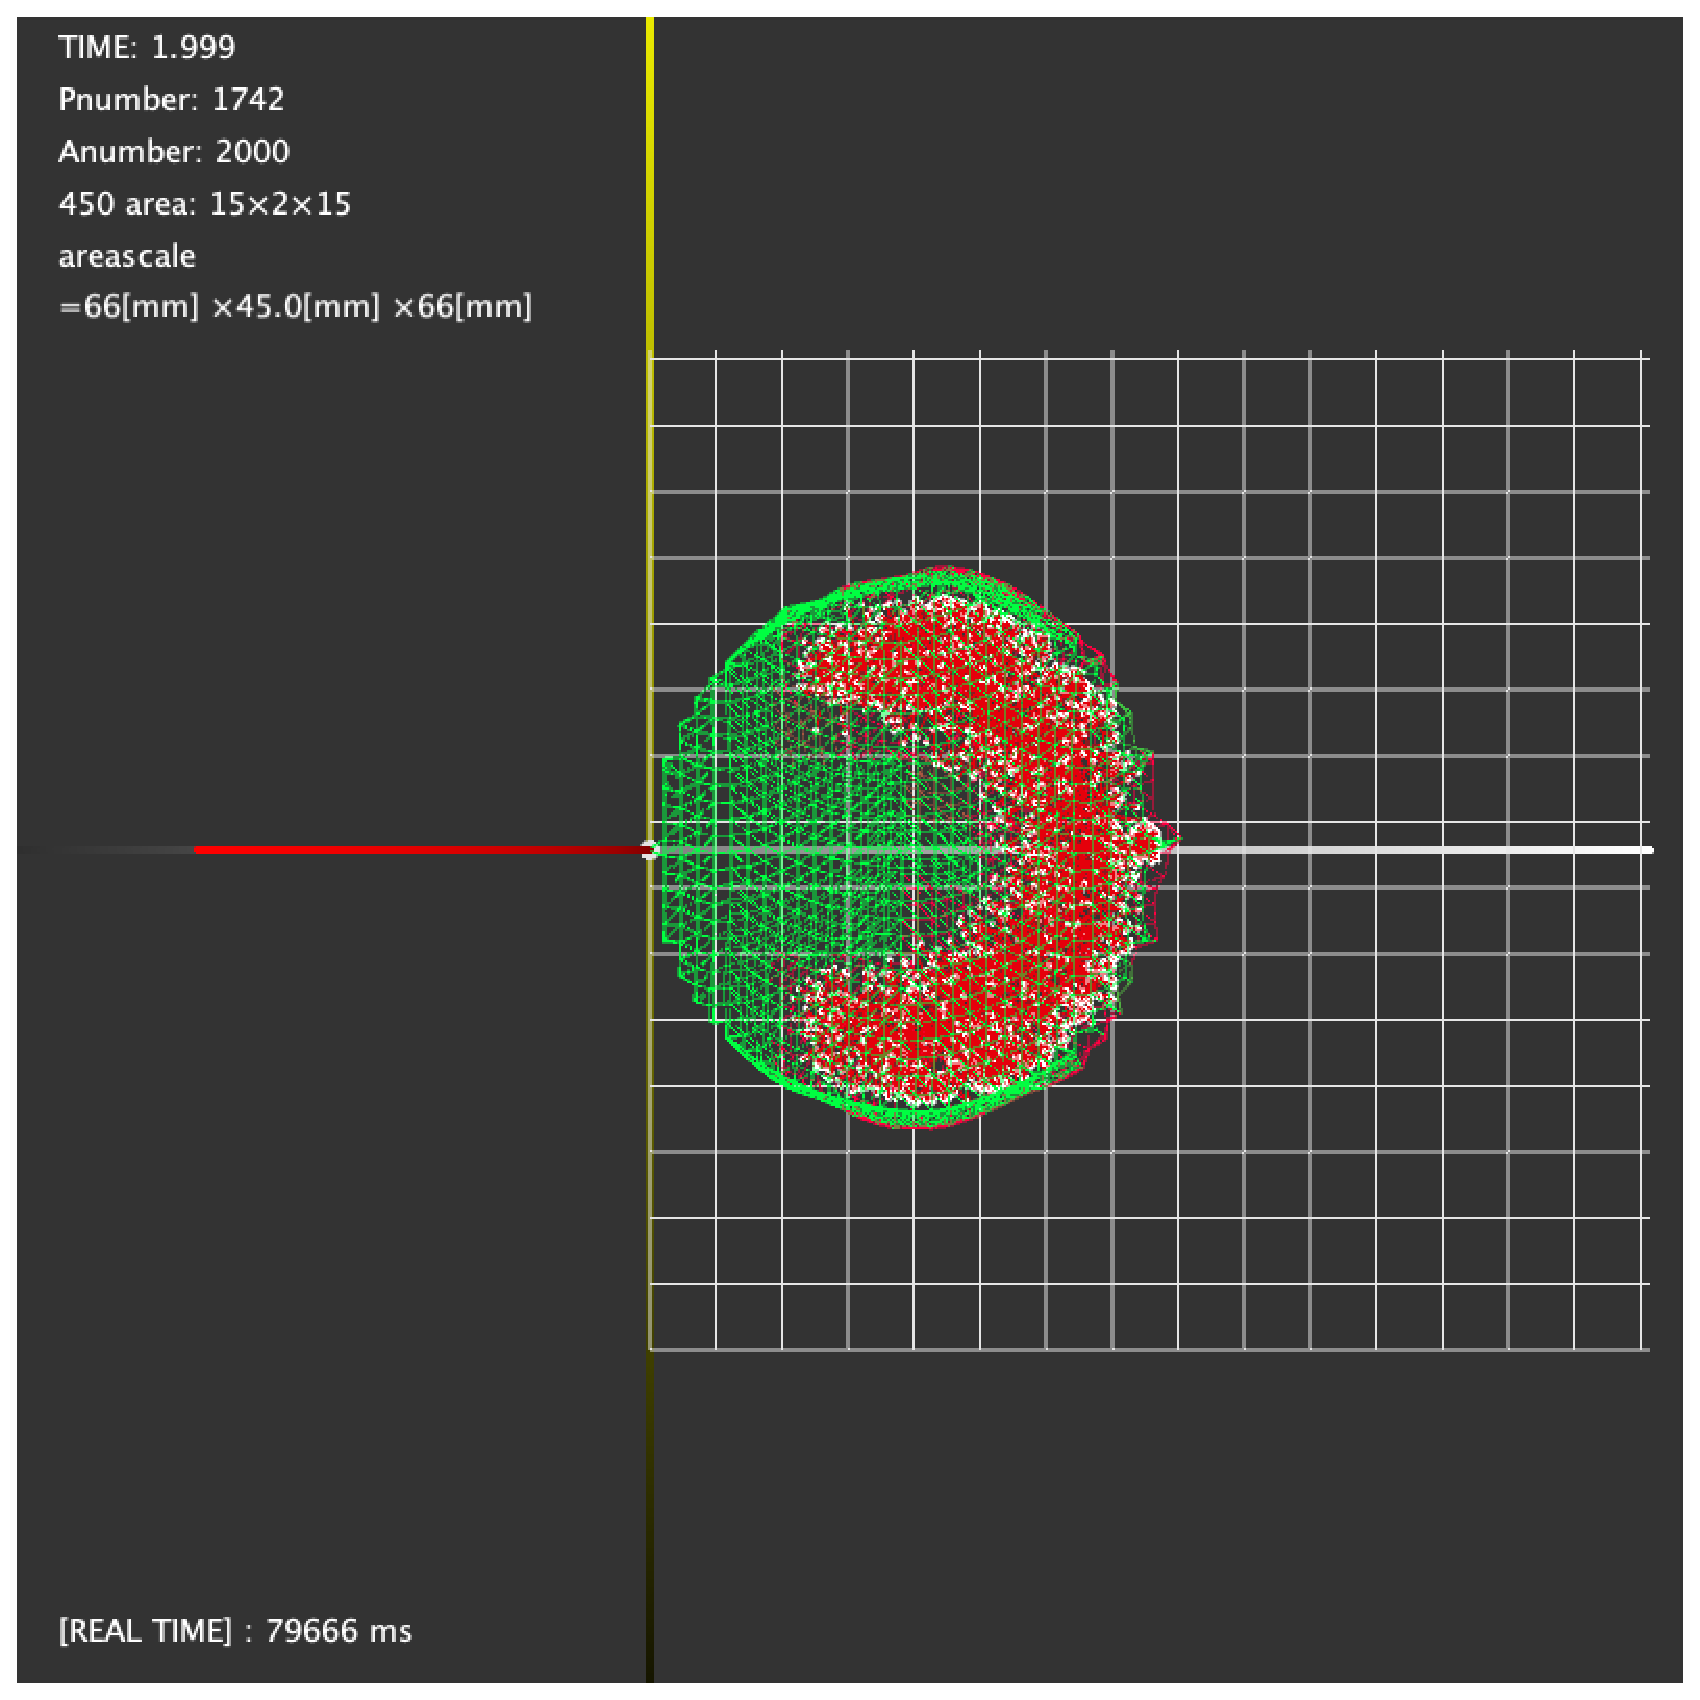
\includegraphics[width=5cm]{top20_25rc.eps} \\
   \includegraphics[width=5cm]{side20_25rc.eps}
  \end{tabular}
 }%
 \subfloat[t=4.0]{%
  \begin{tabular}{c}
   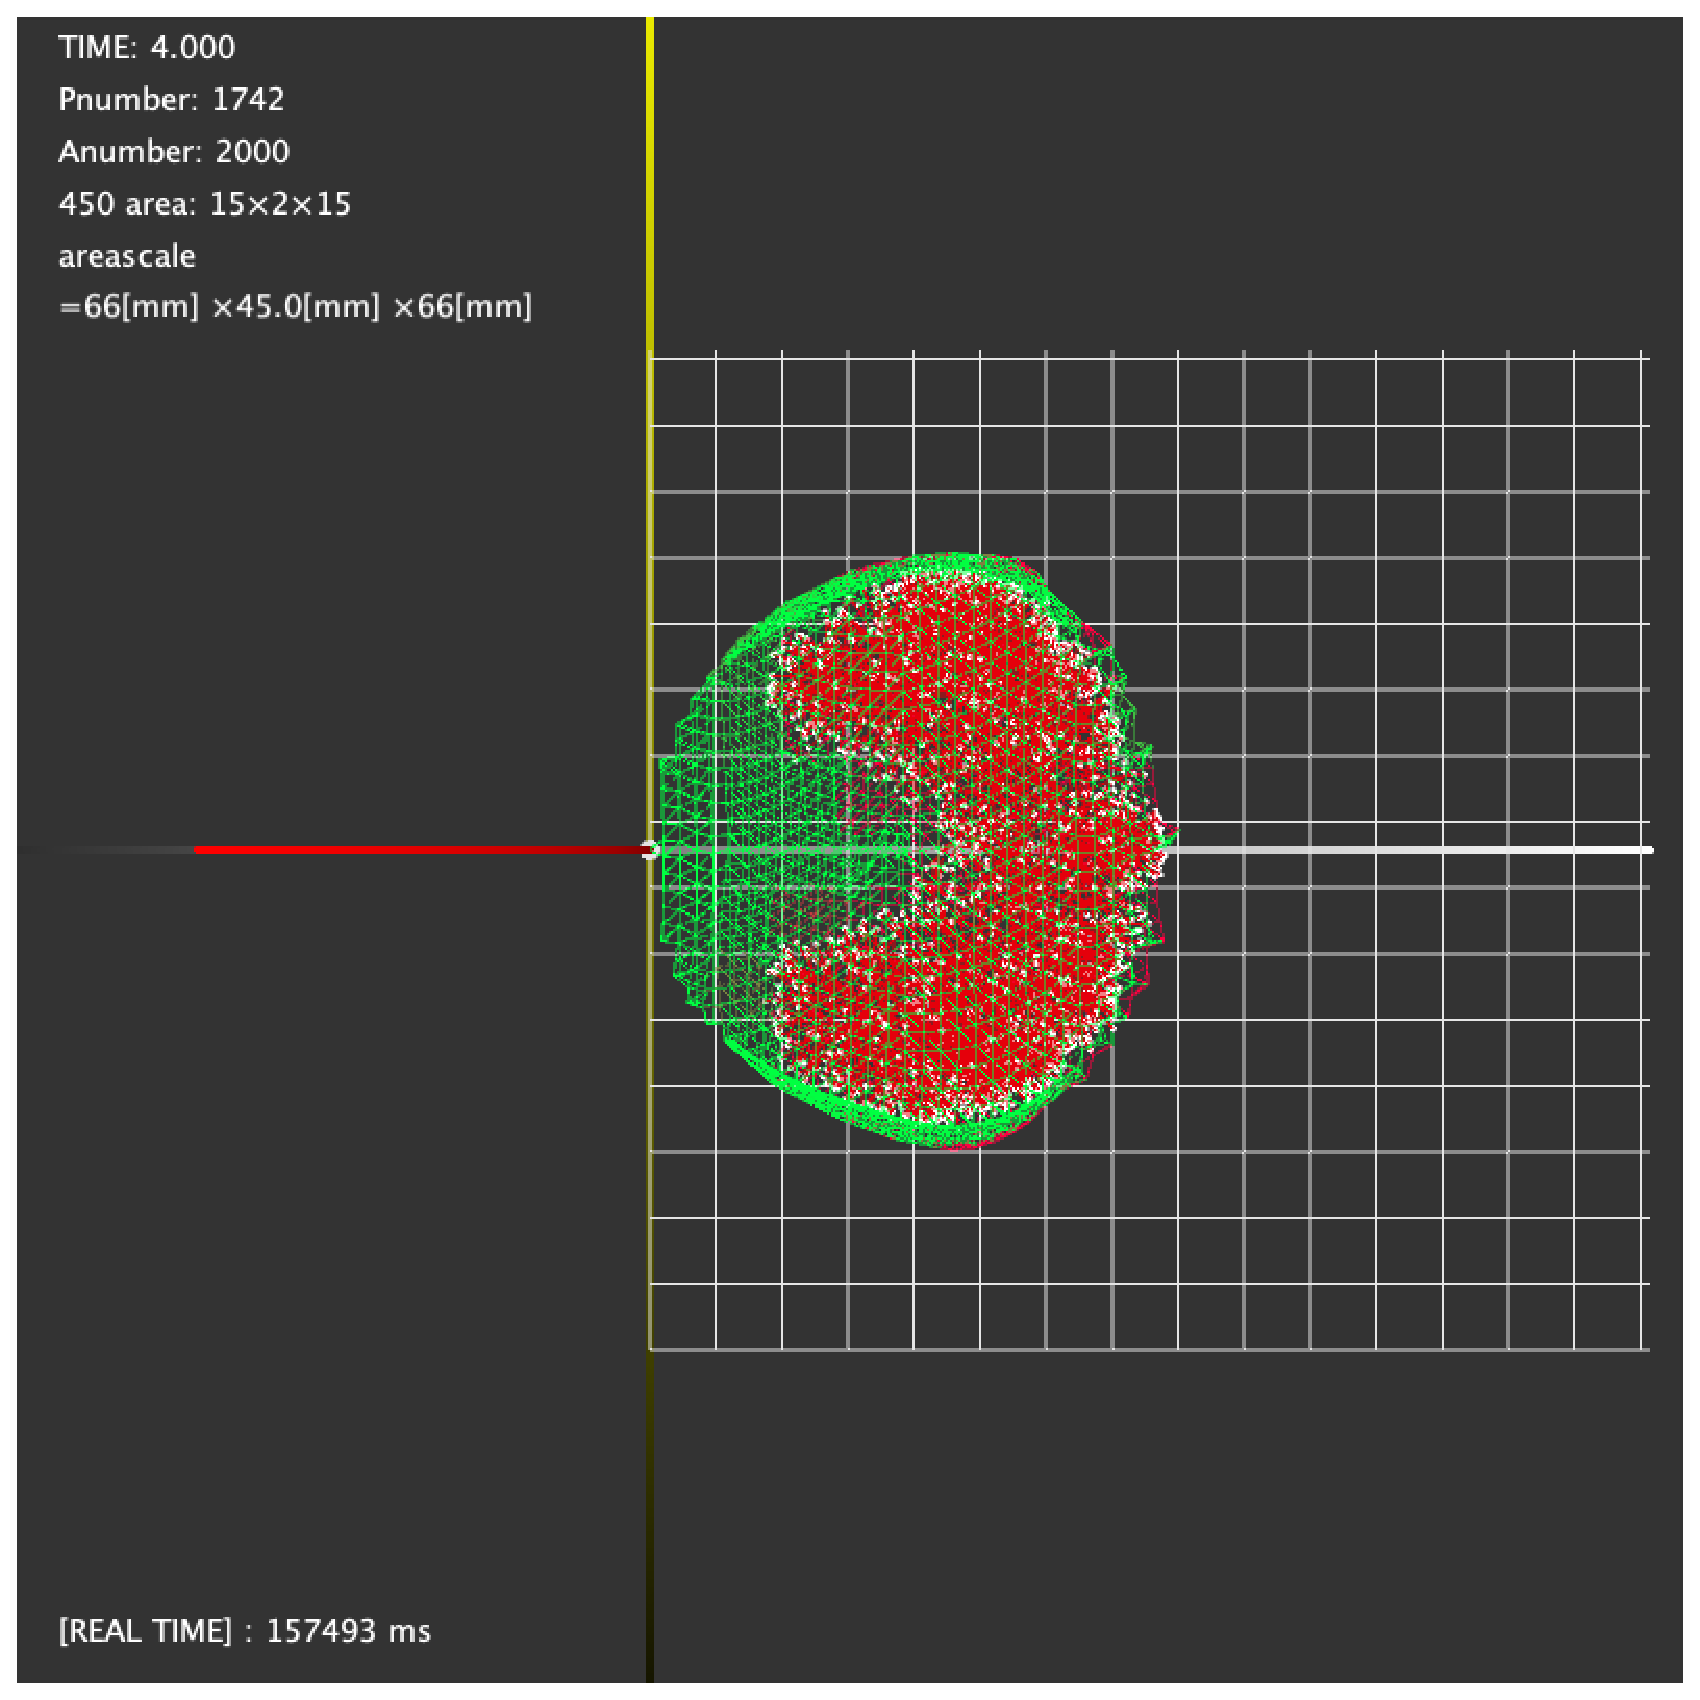
\includegraphics[width=5cm]{top40_25rc.eps} \\
   \includegraphics[width=5cm]{side40_25rc.eps}
  \end{tabular}
 }%
 \caption{Simulation results for relocation condition of actin concentration 2.5\%.}
 \label{fig:res5}
\end{figure}


\begin{figure}[h]
 \subfloat[t=0.5.]{%
  \begin{tabular}{c}
   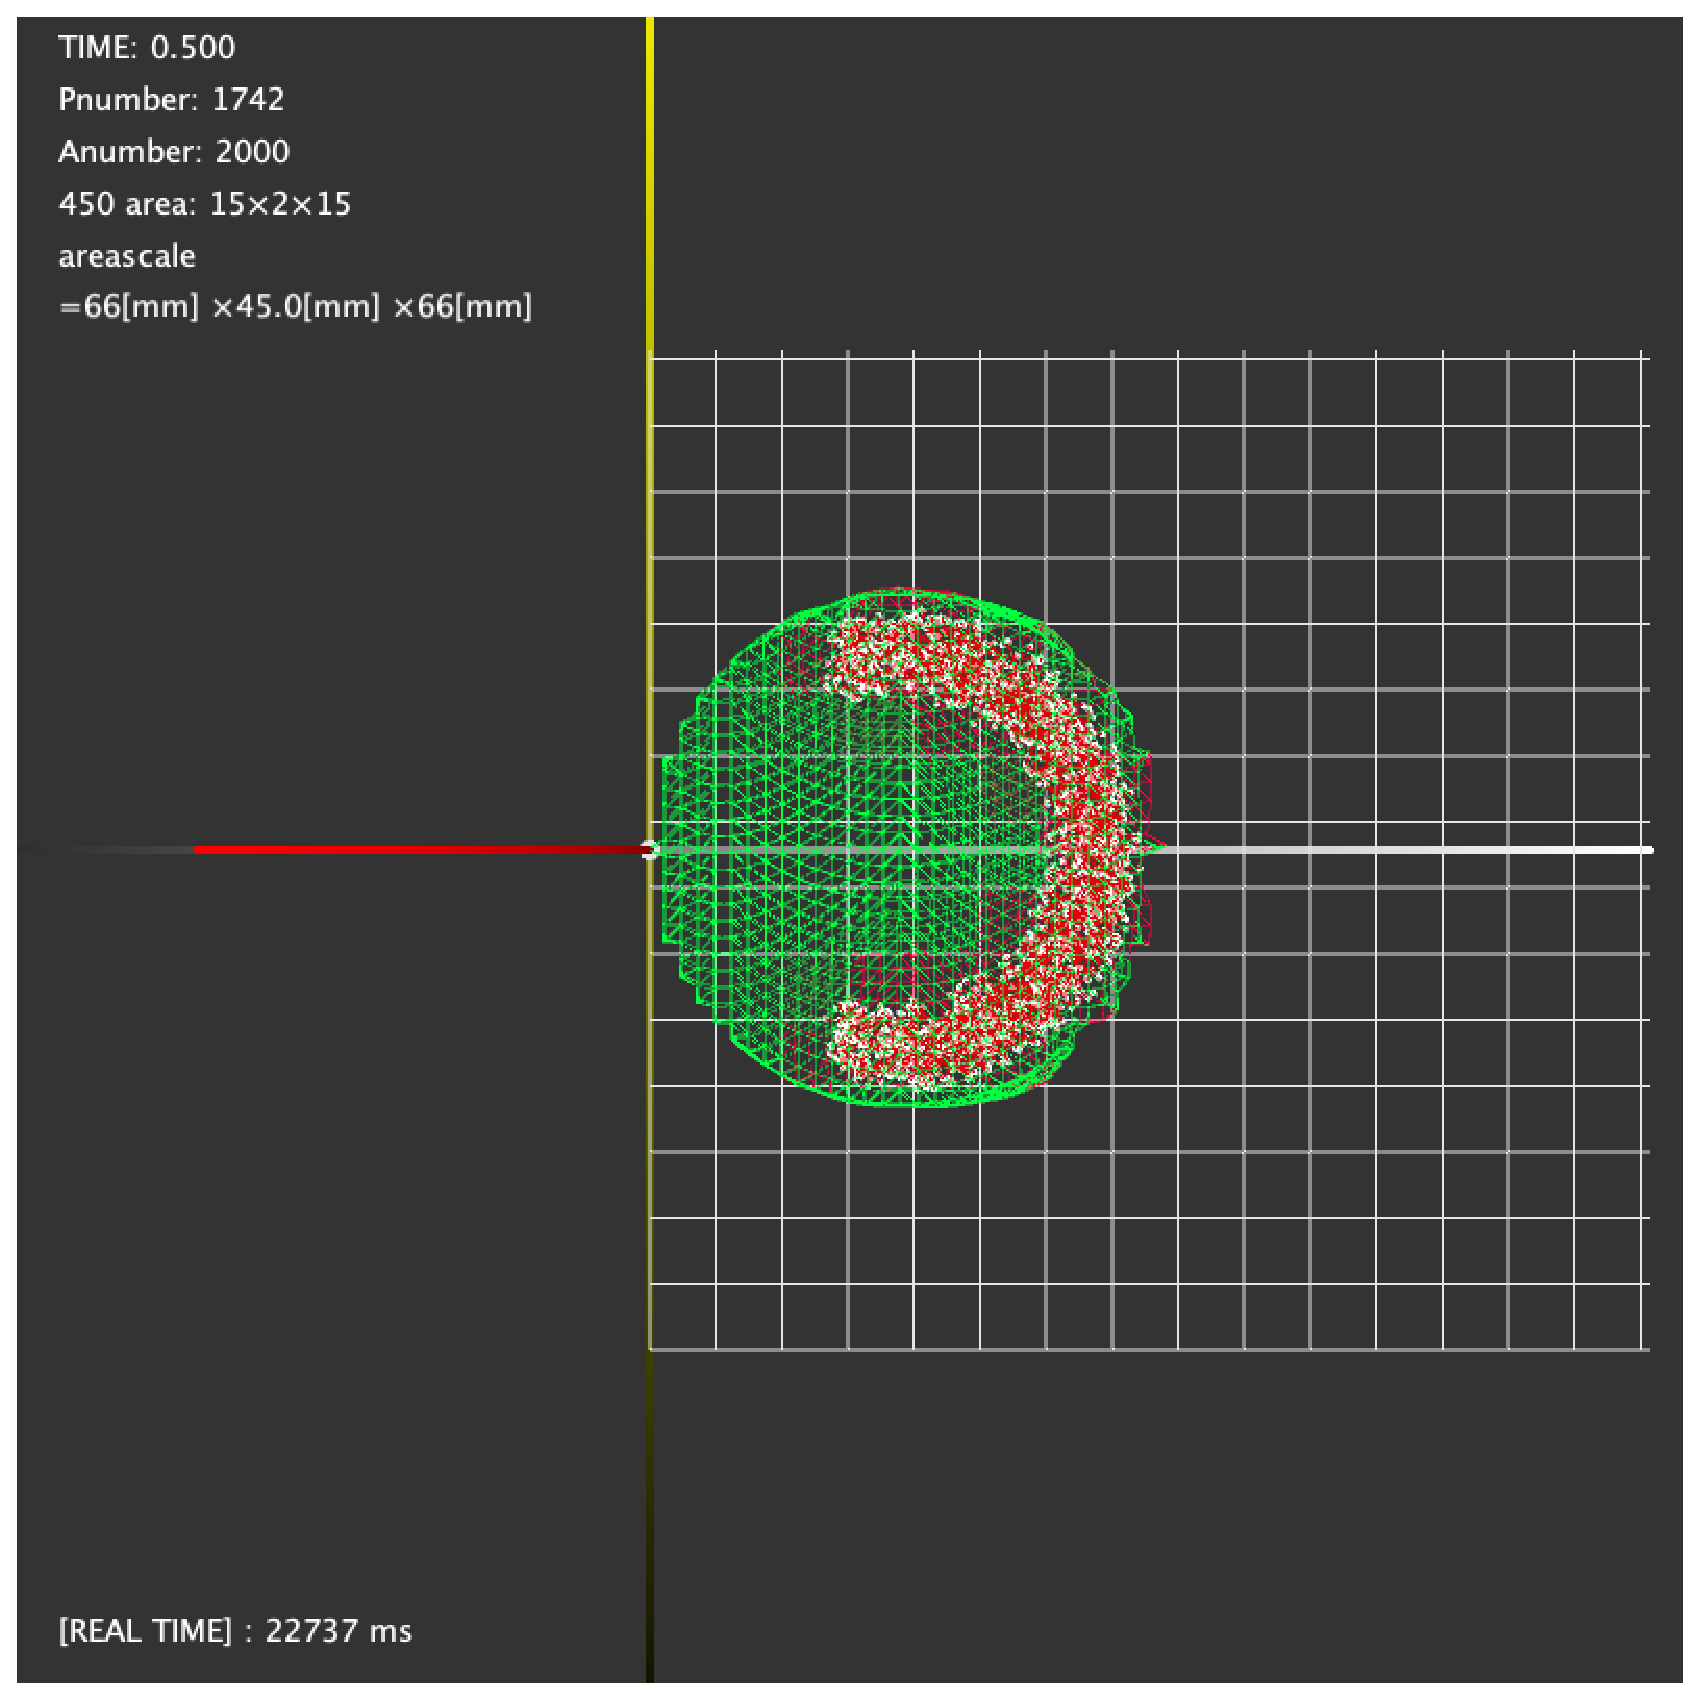
\includegraphics[width=5cm]{top05_30rc.eps} \\
   \includegraphics[width=5cm]{side05_30rc.eps}
  \end{tabular}
 }%
 \subfloat[t=2.0]{%
  \begin{tabular}{c}
   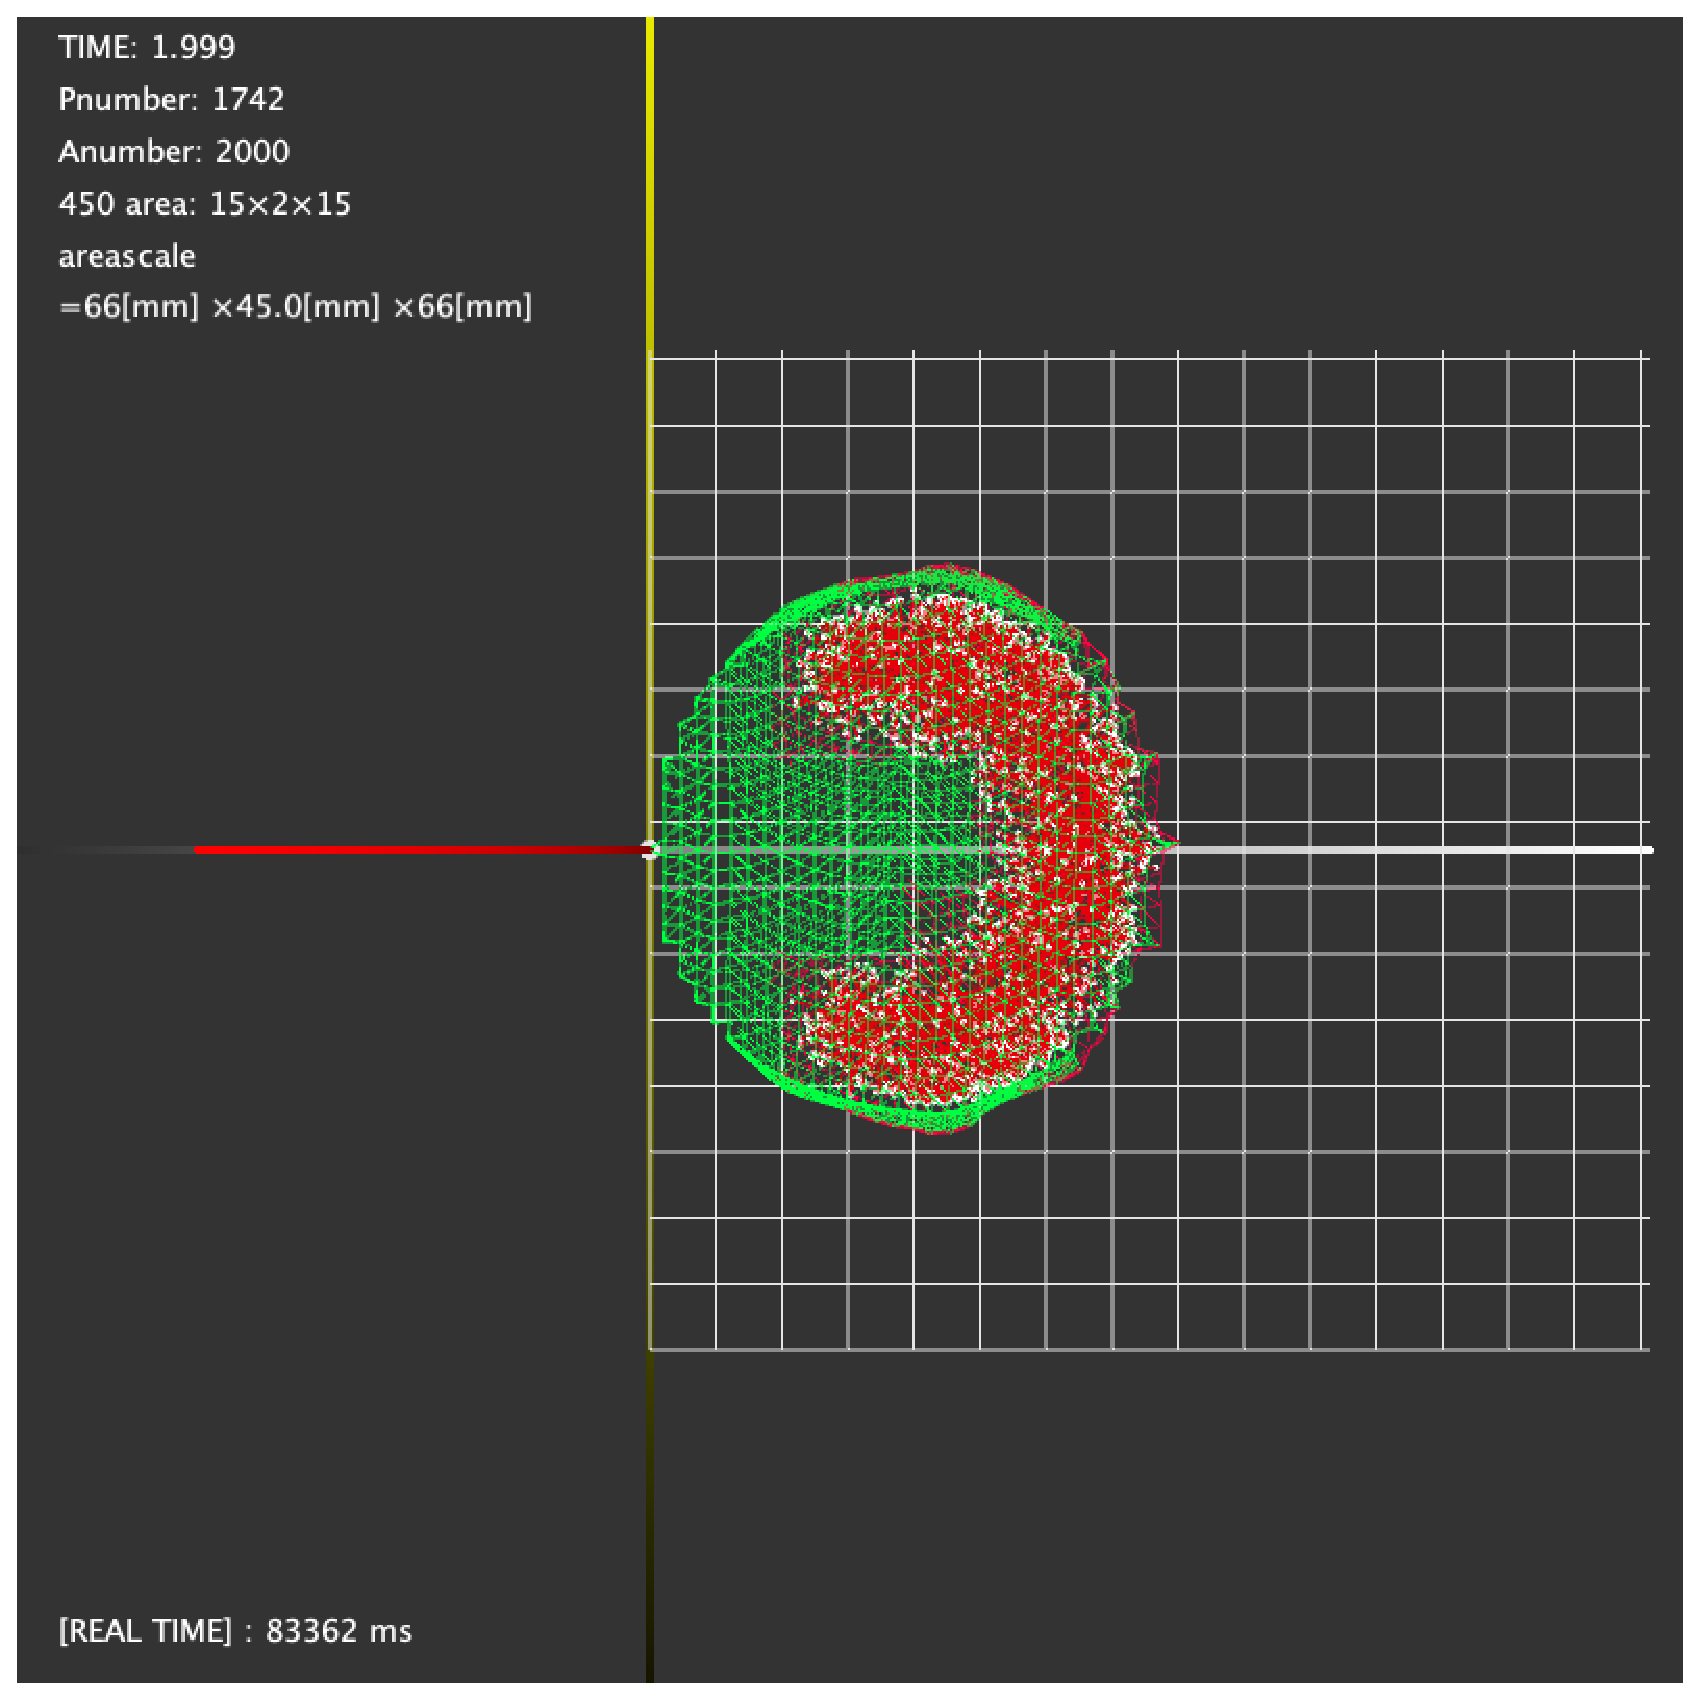
\includegraphics[width=5cm]{top20_30rc.eps} \\
   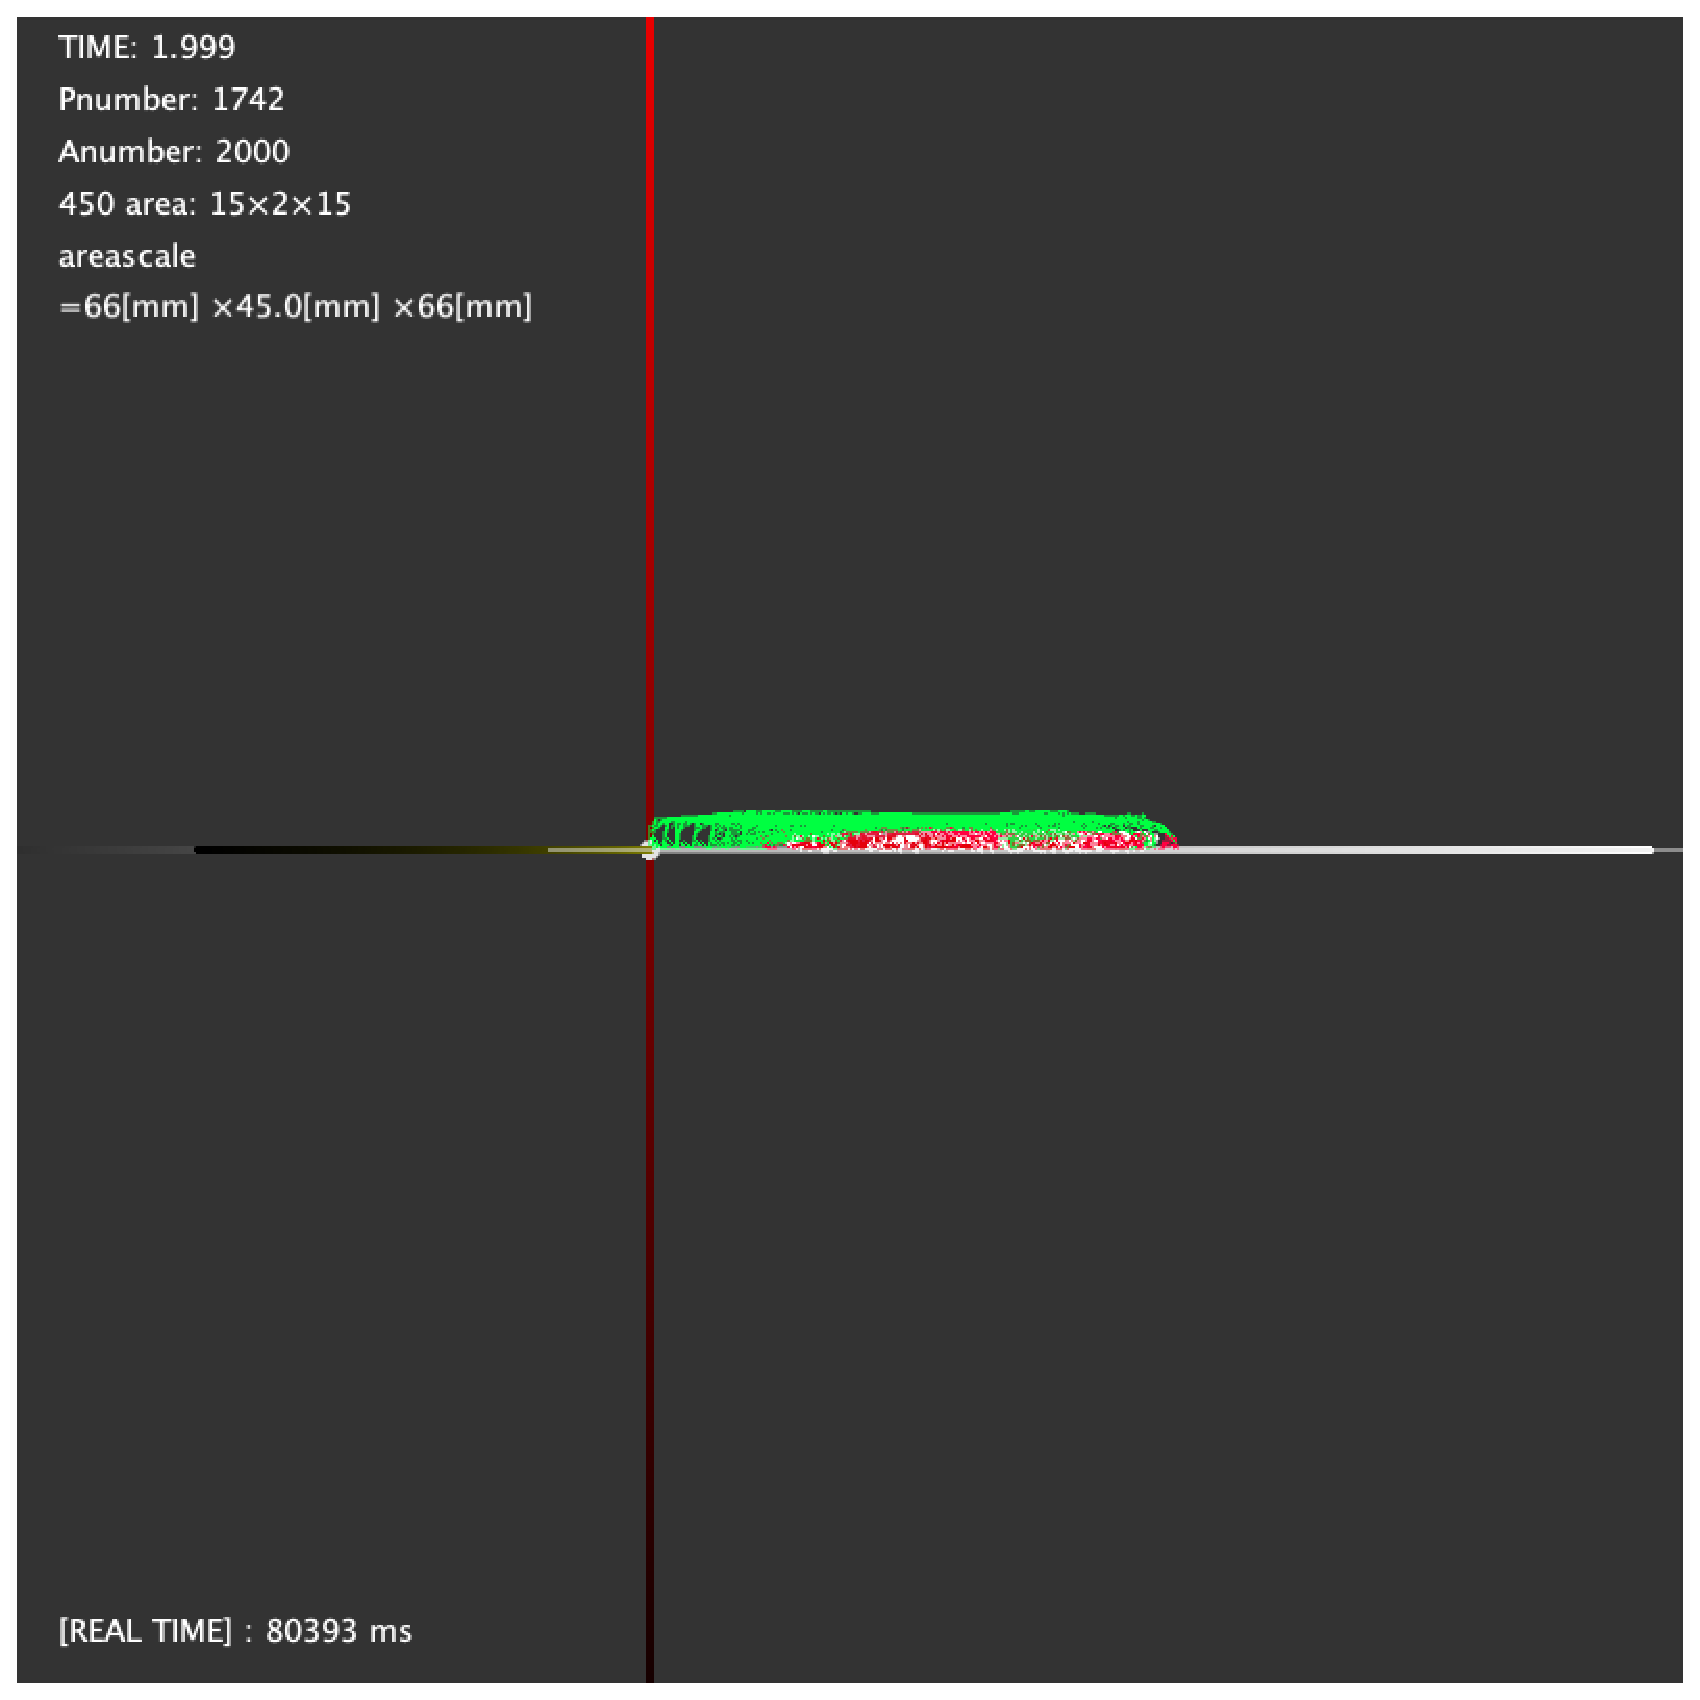
\includegraphics[width=5cm]{side20_30rc.eps}
  \end{tabular}
 }%
 \subfloat[t=4.0]{%
  \begin{tabular}{c}
   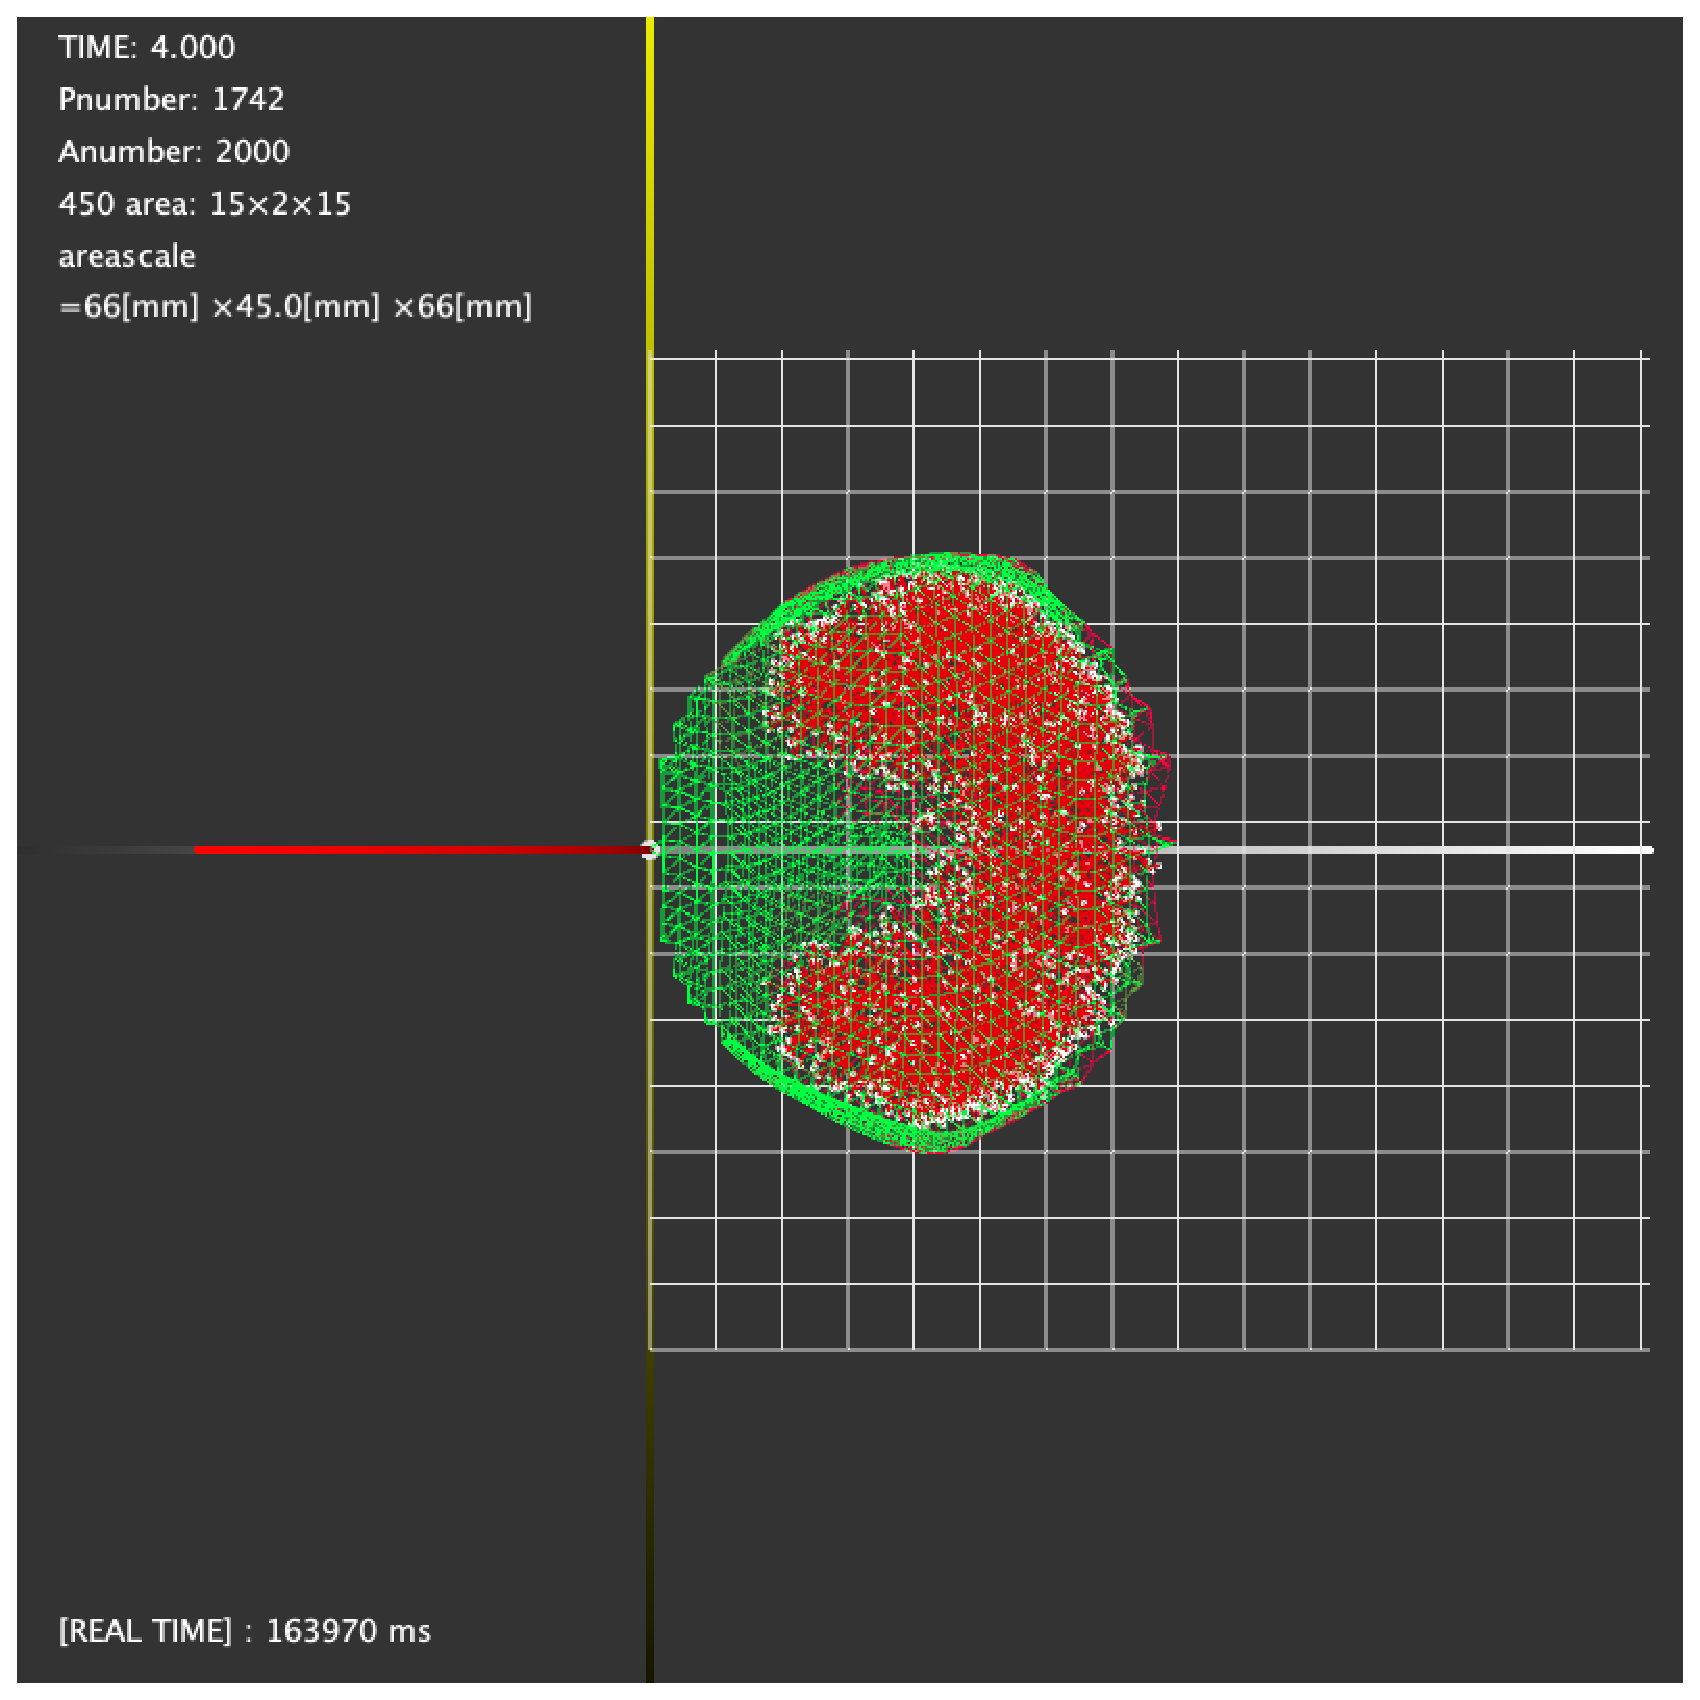
\includegraphics[width=5cm]{top40_30rc.eps} \\
   \includegraphics[width=5cm]{side40_30rc.eps}
  \end{tabular}
 }%
 \caption{Simulation results for relocation condition of actin concentration 3.0\%.}
 \label{fig:res6}
\end{figure}

\subsection{Effect of Initial Placement}

\begin{figure}[h]
 \subfloat[t=0.5.]{%
  \begin{tabular}{c}
   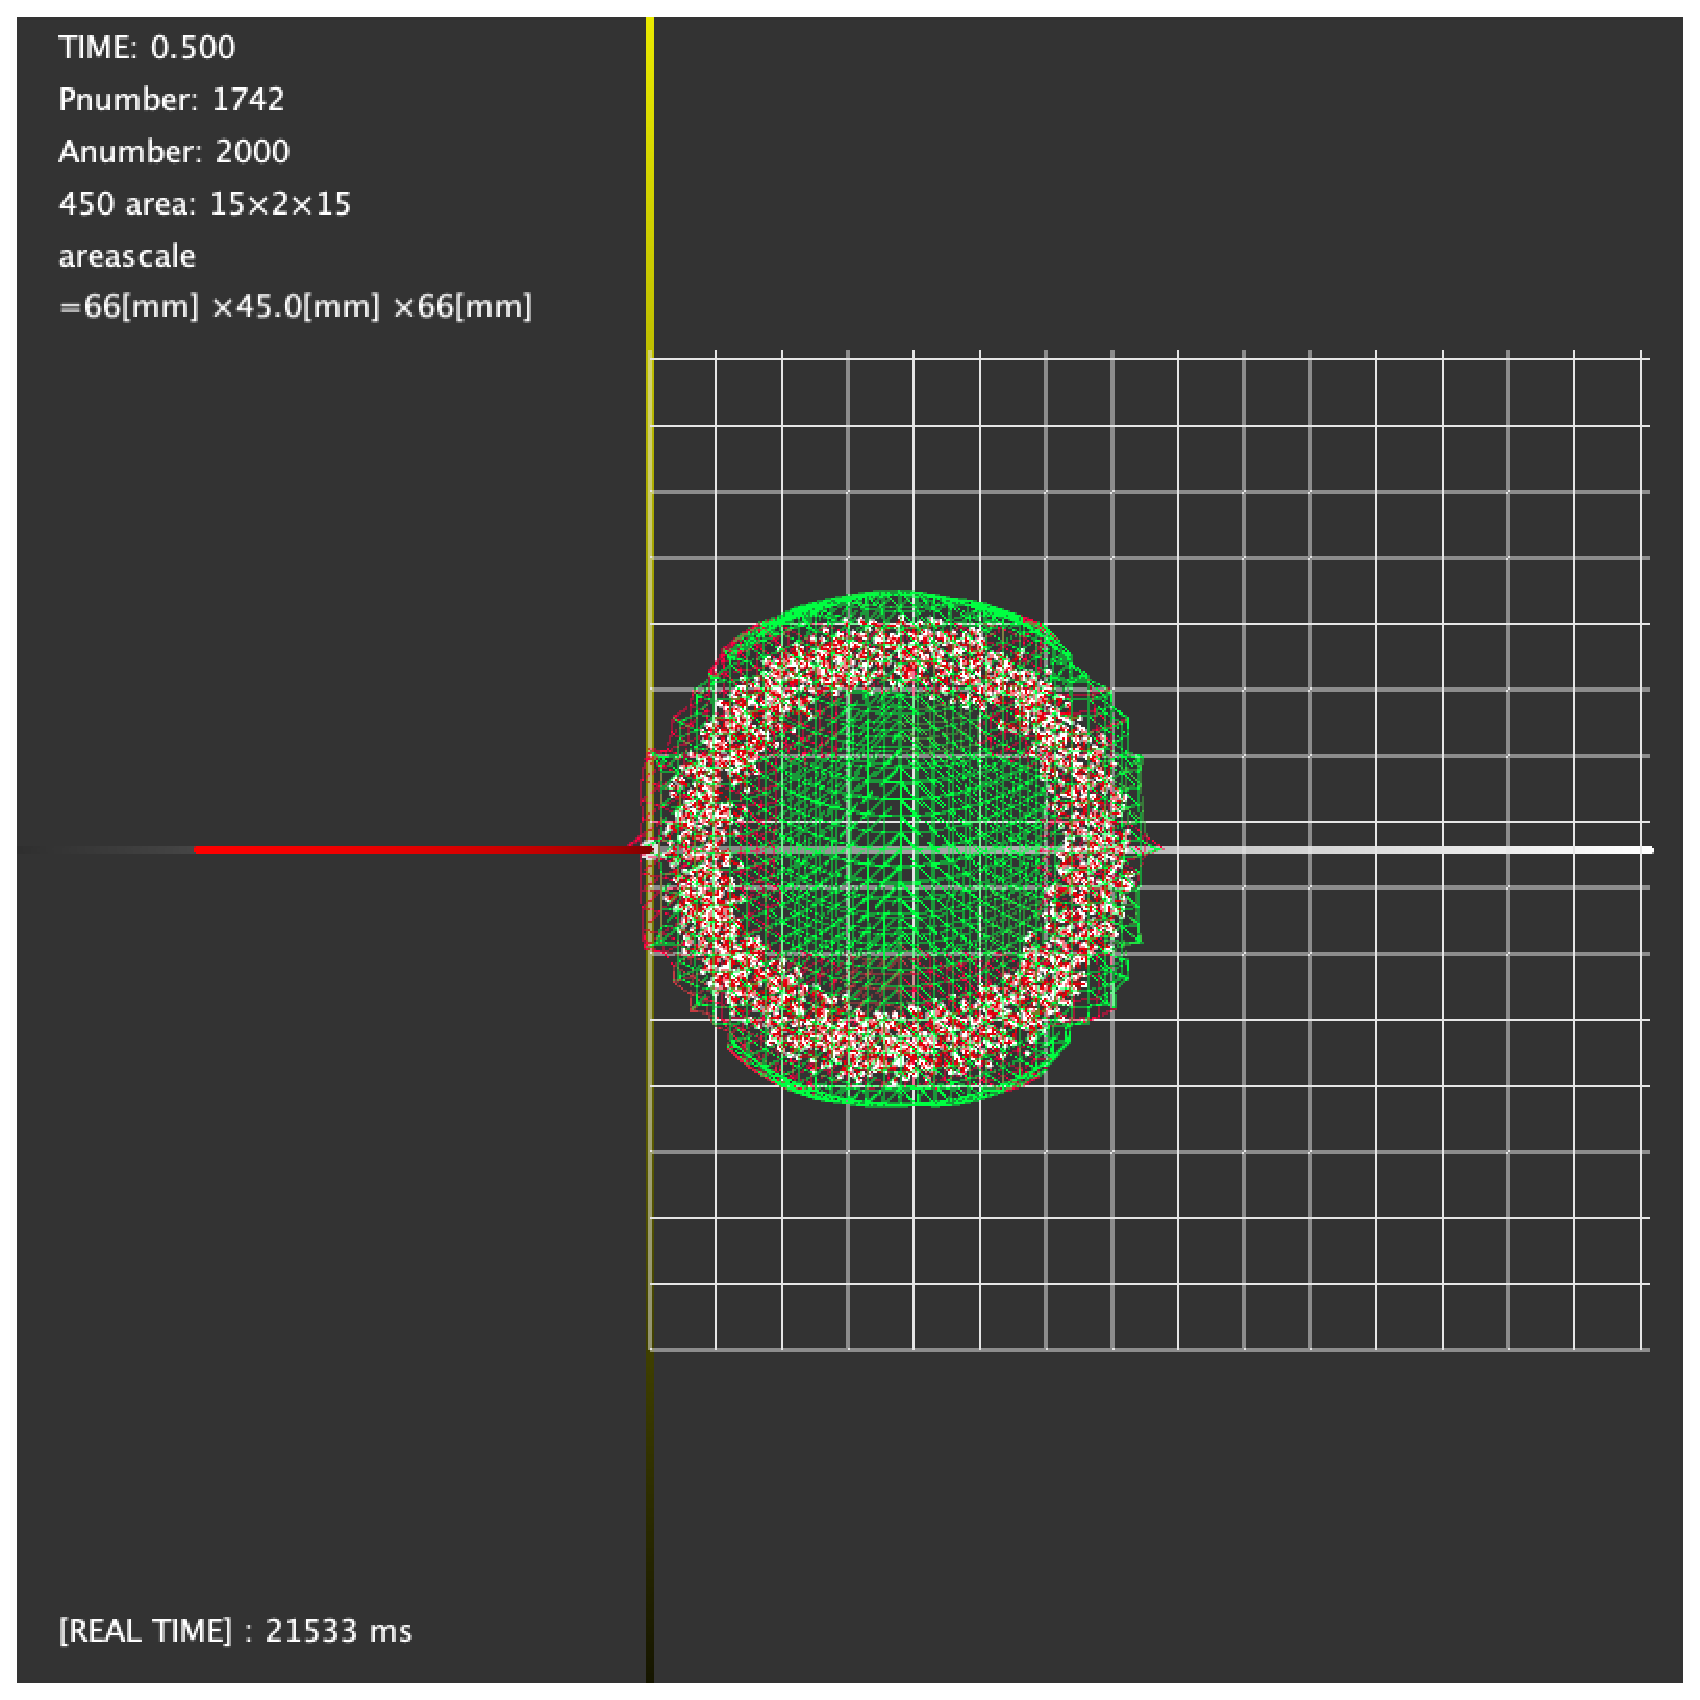
\includegraphics[width=5cm]{top05_ci.eps} \\
   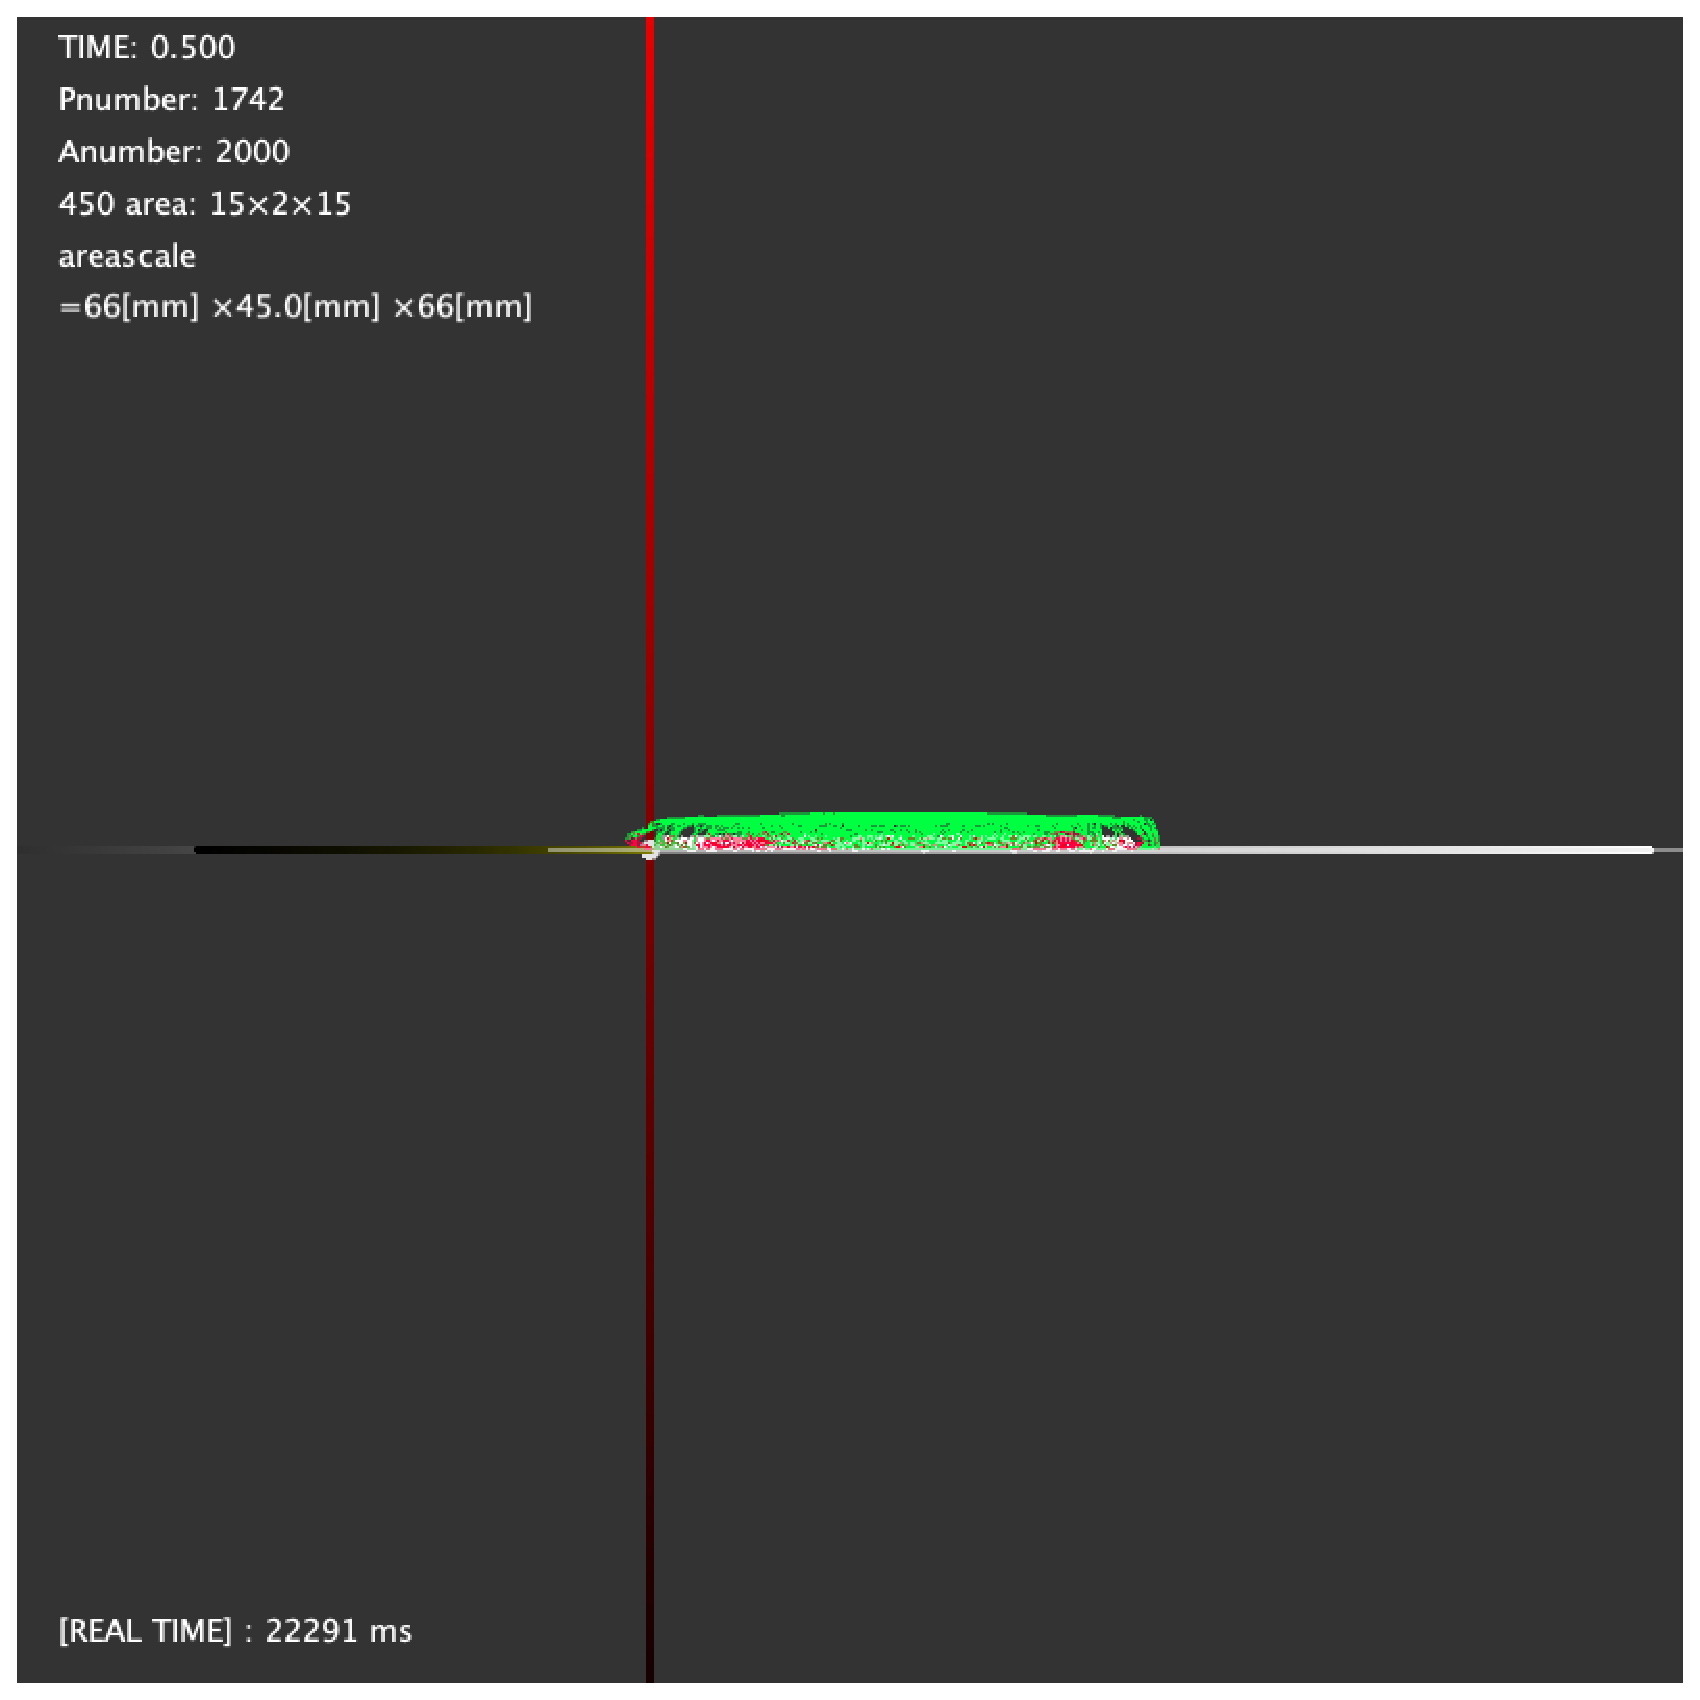
\includegraphics[width=5cm]{side05_ci.eps}
  \end{tabular}
 }%
 \subfloat[t=2.0]{%
  \begin{tabular}{c}
   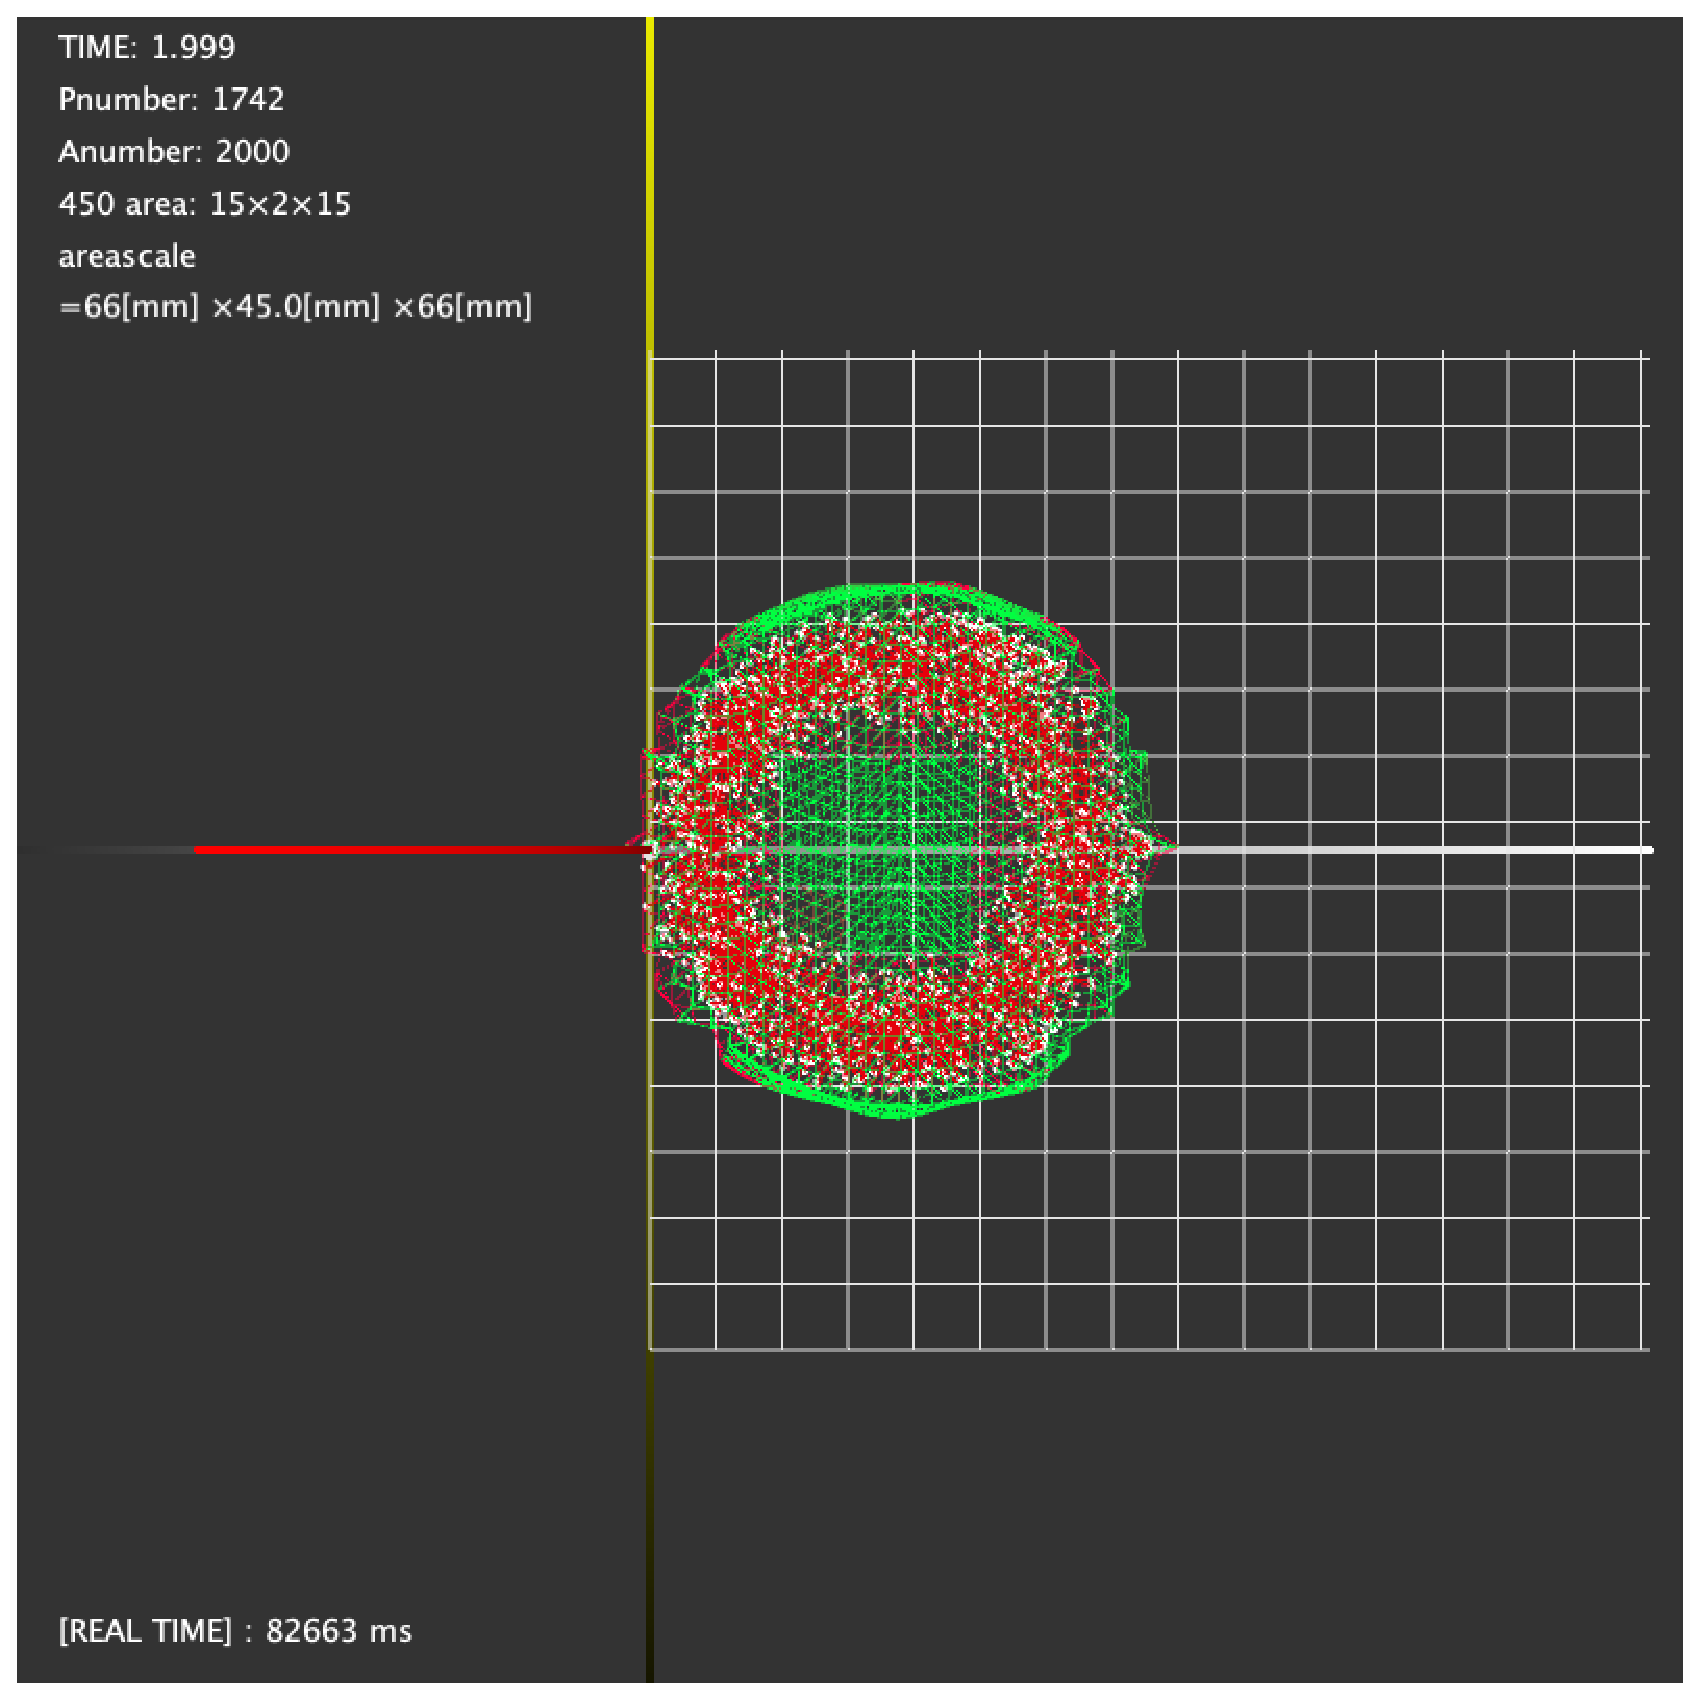
\includegraphics[width=5cm]{top20_ci.eps} \\
   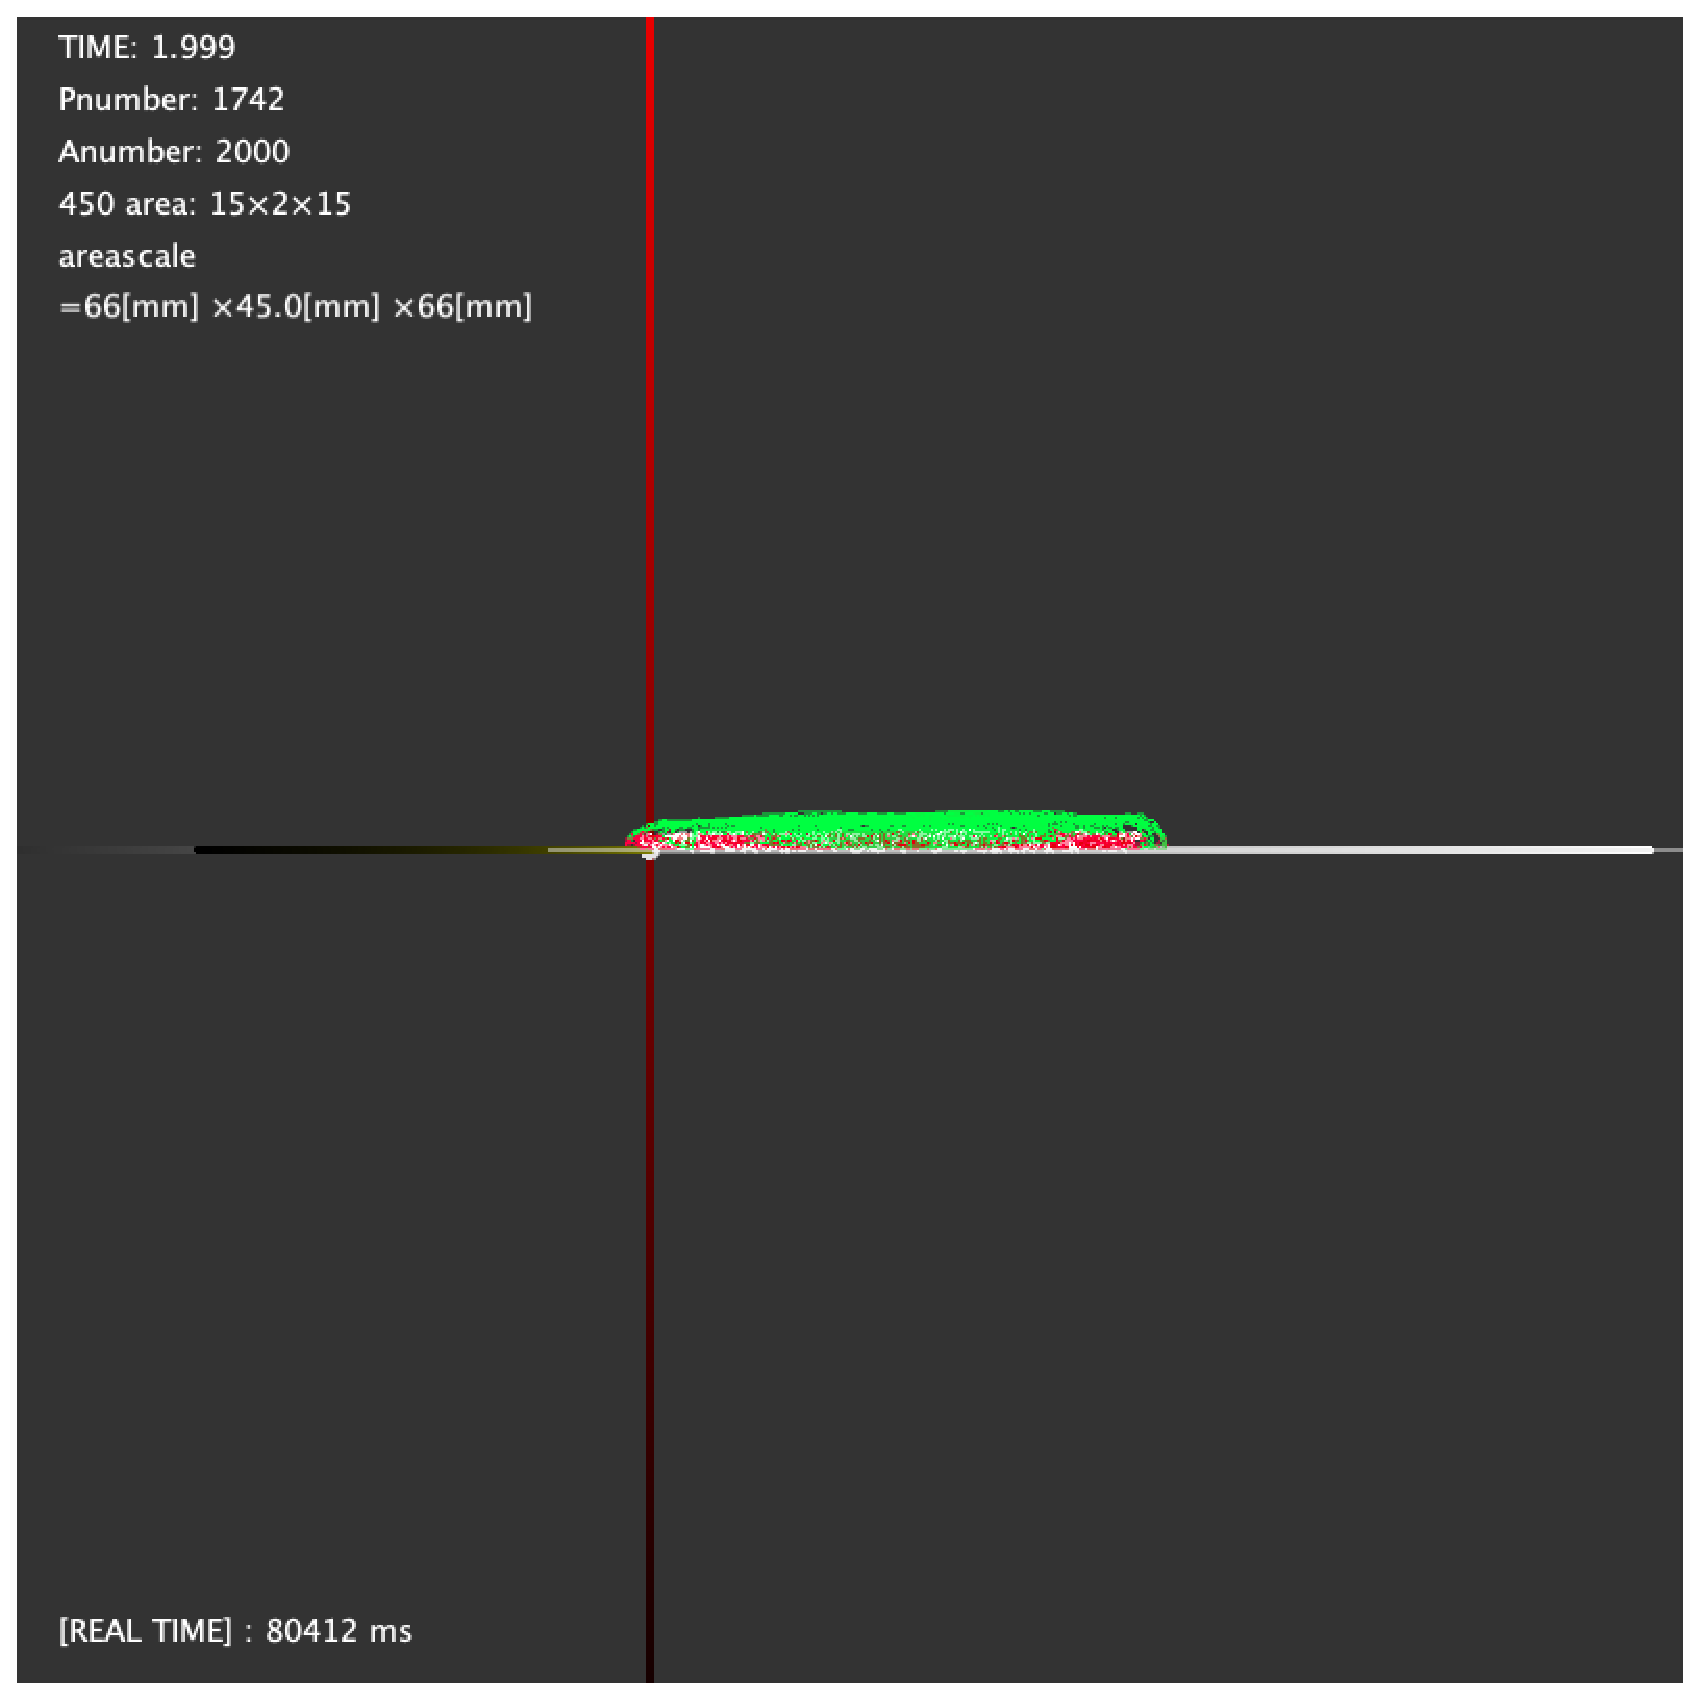
\includegraphics[width=5cm]{side20_ci.eps}
  \end{tabular}
 }%
 \subfloat[t=4.0]{%
  \begin{tabular}{c}
   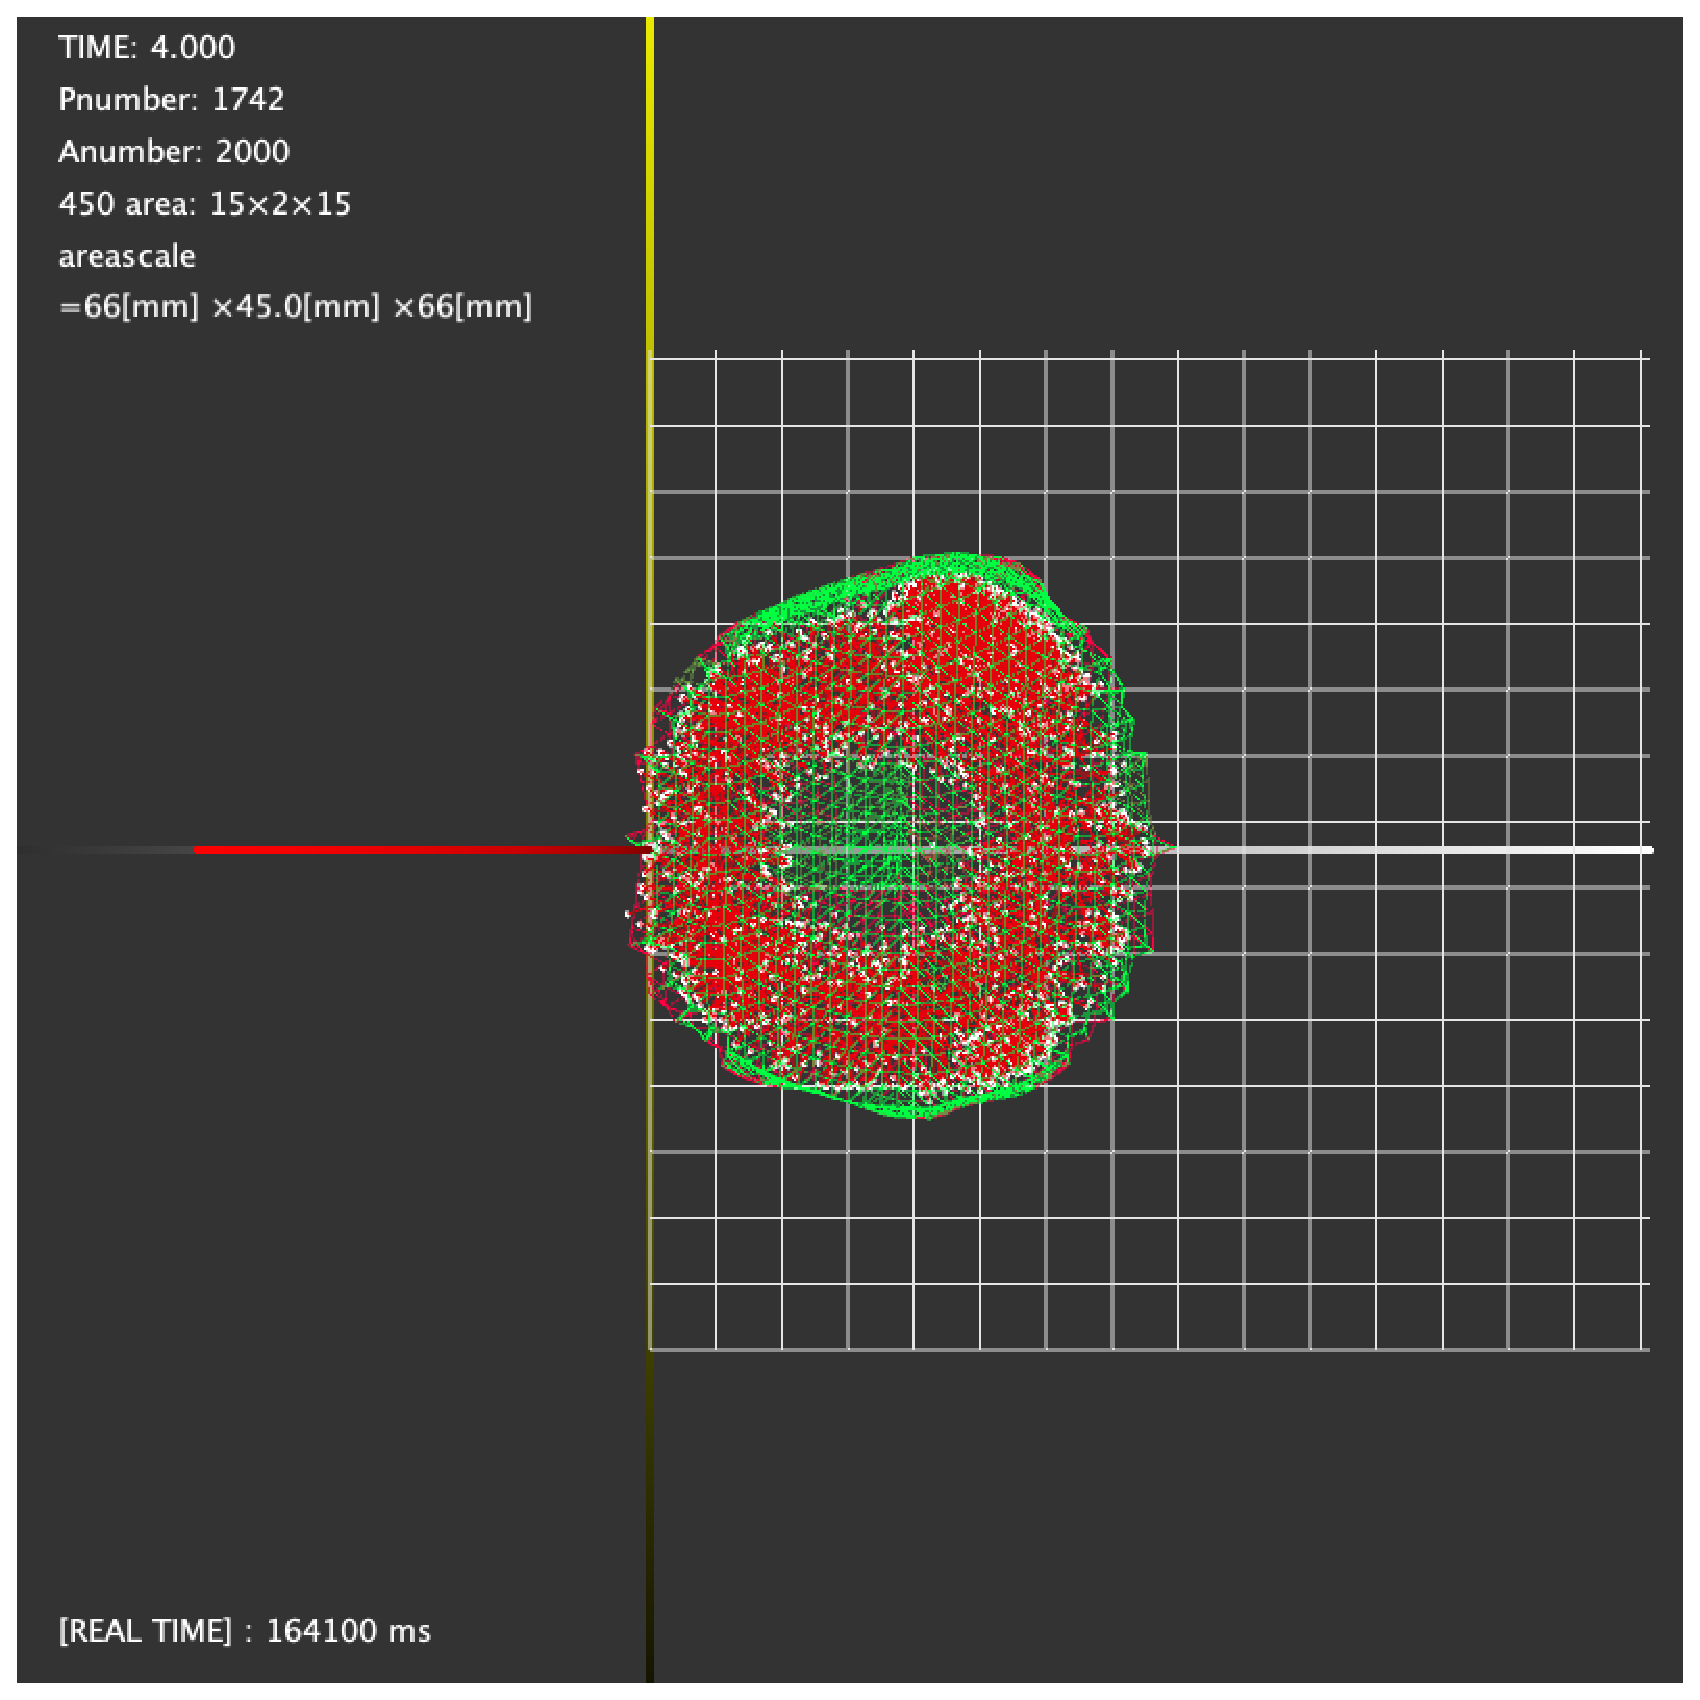
\includegraphics[width=5cm]{top40_ci.eps} \\
   \includegraphics[width=5cm]{side40_ci.eps}
  \end{tabular}
 }%
 \caption{Simulation results when the initial arrangement of actin molecules is circular.}
 \label{fig:res7}
\end{figure}


\section{Discussion}
The cell membrane molecule undergoes both the force from the actin molecule and the force of the nearby membrane molecule simultaneously. Therefore, when the actin molecule is excessively polymerized, the cell membrane can not be flexibly deformed, so it ruptures. This result suggests that ARF alleviates the excessive load on the cell membrane by regressing actin molecule.

\chapter{Conclusions and Future Work}
\section{Morphology of Keratocytes and Its Motor Function}

\section{Future Prospects}

\chapter*{Acknowledgements}
We gratefully acknowledge the work of past and present members of our laboratory.

\addcontentsline{toc}{chapter}{Acknowledgements}
\bibliography{bibtexfile.bib}
\bibliographystyle{junsrt}

\addcontentsline{toc}{chapter}{\bibname}
\end{document}
